\documentclass[12pt]{uthesis-v12}  %---> DO NOT ALTER THIS COMMAND

\usepackage{graphicx}

% *** GRAPHICS RELATED PACKAGES ***
%
%\ifCLASSINFOpdf
 % \usepackage[pdftex]{graphicx}
  % declare the path(s) where your graphic files are
\graphicspath{{figures/pdf/}{figures/eps/}}
  % and their extensions so you won't have to specify these with
  % every instance of \includegraphics
  %\DeclareGraphicsExtensions{.pdf,.jpeg,.png}
%\else
  % or other class option (dvipsone, dvipdf, if not using dvips). graphicx
  % will default to the driver specified in the system graphics.cfg if no
  % driver is specified.
 % \usepackage[dvips]{graphicx}
  % declare the path(s) where your graphic files are
  %\graphicspath{{../eps/}}
  % and their extensions so you won't have to specify these with
  % every instance of \includegraphics
  %\DeclareGraphicsExtensions{.eps}
%\fi

\usepackage{mathtools}

\usepackage{subfig}
\usepackage{algorithmic}
\usepackage{booktabs}
\usepackage{epstopdf}
\usepackage[T1]{fontenc}
%\usepackage[margin=1in]{geometry}
\usepackage{array}
\newcolumntype{L}[1]{>{\raggedright\let\newline\\\arraybackslash\hspace{0pt}}m{#1}}

%\renewcommand{\arraystretch}{1.2}

\usepackage{float}
\newfloat{algorithm}{t}{lop}
\floatname{algorithm}{Algorithm}
\usepackage{xpatch}

\usepackage{accents}
\newcommand{\ubar}[1]{\underaccent{\bar}{#1}}



%% The amssymb package provides various useful mathematical symbols
\usepackage{amssymb}
\usepackage{cleveref}
\usepackage{cite}
%\usepackage{setspace}


\usepackage[labelsep=colon]
                %labelfont={sf,bf},
                %textfont=sf]
               {caption}
\captionsetup{format=hang}    

\usepackage[numbers,sort&compress]{natbib}           

%\makeatletter
%\xpatchcmd{\algorithmic}{\itemsep\z@}{\itemsep=1ex plus0.5pt}{}{}
%\makeatother

\begin{document} %---> %---> %---> %---> DO NOT ALTER THIS COMMAND

%--------+----------------------------------------------------------+
%        |  \title{}                                    (REQUIRED)  |
%        |  \author{}                                   (REQUIRED)  |
%        |                                                          |
%        |  See section 3.1 of "Read_Me_First_(v12).pdf"            |
%        |                                                          |
%        |  Also see section 2.2 of above "Read Me" file for the    |
%        |  proper use of the invisible tilde ("~") character when  |
%        |  entering a middle initial in the \author command.       |
%        +----------------------------------------------------------+

\title{Development of Adaptive Computational Algorithms for Manned and Unmanned Flight Safety}

\author{Colin P.~Elkin}

%--------+----------------------------------------------------------+
%        |  \copyrightpage{}                            (REQUIRED)  |
%        |                                                          |
%        |  See section 3.2 of "Read_Me_First_(v12).pdf"            |
%        |                                                          |
%        |  1) You must enter either "yes" or "no" in this          |
%        |      command.  Inputting "yes" produces a copyright      |
%        |      notification page as the second page and inputting  |
%        |      "no" produces a blank second page.                  |
%        |  2) Input to this command is case sensitive.             |
%        |  3) Default: the "yes" option.                           |
%        +----------------------------------------------------------+

\copyrightpage{yes}

%--------+----------------------------------------------------------+
%        |  \mydocument{}                               (REQUIRED)  |
%        |                                                          |
%        |  See section 3.3 of "Read_Me_First_(v12).pdf"            |
%        |                                                          |
%        |  1) Input to this command is limited to the following    |
%        |     three options: a) Dissertation                       |
%        |                    b) Thesis                             |
%        |                    c) Project                            |
%        |  2) Input to this command is case-sensitive.             |
%        +----------------------------------------------------------+

\mydocument{Dissertation}

%--------+----------------------------------------------------------+
%        |  \degree{}{}                                 (REQUIRED)  |
%        |                                                          |
%        |  See section 3.4 of "Read_Me_First_(v12).pdf"            |
%        |                                                          |
%        |  You need to provide two distinct inputs into this       |
%        |  command:                                                |
%        |     1) In the first set of braces you need to specify    |
%        |        the *exact* degree you will receive. Some         |
%        |        examples are: -) Masters of Arts                  |
%        |                      -) Masters of Science               |
%        |                      -) Doctor of Philosophy             |
%        |     2) In the second set of braces you need to state the |
%        |        *specific* discipline or area for that degree     |
%        |        (e.g., Economics, Education, Engineering, etc.).  |
%        |  Students should consult their advisor if they have any  |
%        |  questions about this information.                       |
%        +----------------------------------------------------------+

\degree{Doctor of Philosophy}{Engineering}

%--------+----------------------------------------------------------+
%        |  \conferraldate{}{}                          (REQUIRED)  |
%        |                                                          |
%        |  See section 3.5 of "Read_Me_First_(v12).pdf"            |
%        |                                                          |
%        |  In the two set of braces enter the month and then the   |
%        |  year your degree will be *conferred* by the university. |
%        +----------------------------------------------------------+

\conferraldate{December}{2018}

%--------+----------------------------------------------------------+
%        |  \advisor{}                                  (REQUIRED)  |
%        |                                                          |
%        |  See section 3.6.2 of "Read_Me_First_(v12).pdf"          |
%        |                                                          |
%        |  1) Also see section 2.2 of "Read_Me_First_(v12).pdf"    |
%        |     for the proper use of the invisible tilde ("~")      |
%        |     character when entering a middle initial or the      |
%        |     abbreviation of an academic title (e.g., Dr.) in     |
%        |     the \advisor{} command.                              |
%        |  2) Also see section 3.6.1. for consistent presentation  |
%        |     of title page signature lines.                       |
%        +----------------------------------------------------------+

\advisor{Dr.~Vijay Devabhaktuni}

%--------+----------------------------------------------------------+
%        |  Committee Member Signature Commands         (OPTIONAL)  |
%        |                                                          |
%        |  See section 3.6.3 of "Read_Me_First_(v12).pdf"          |
%        |                                                          |
%        |  1) Use the commands below to provide signature lines    |
%        |     for your "other" committee members;                  |
%        |        --> you must list your other committee members    |
%        |            in alphabetic order by last name              |
%        |        --> to do this, use the commands below in the     |
%        |            order presented below.                        |
%        |  2) You can choose to include none, some, or all of the  |
%        |     "XXXmember" commands below --- based on the number   |
%        |     committee members you have; simply delete (or        |
%        |     comment-out) any of the commands below that are not  |
%        |     needed.                                              |
%        |  3) Do not include the name of your committee chair or   |
%        |     the Graduate Dean in the commands listed below.      |
%        |     Their signature lines are generated by the           |
%        |     \advisor{} and \graduatedean{}{} commands.           |
%        |  4) You cannot use any of the commands below more than   |
%        |     once. (For details on this issue, see section 3.6.3  |
%        |     of "Read_Me_First_(v12).pdf".)                       |
%        |  5) Also see section 2.2 of "Read_Me_First_(v12).pdf"    |
%        |     for the proper use of the invisible tilde ("~")      |
%        |     character when entering a middle initial or the      |
%        |     abbreviation of an academic title (e.g., Dr.) in     |
%        |     the commands below.                                  |
%        |  6) See section 3.6.1. for consistent presentation of    |
%        |     title page signature lines.                          |
%        |                                                          |
%        |  I know I shouldn't have to say this, but enough         |
%        |  students over the years have made the same mistake      |
%        |  that I'm forced to state:                               |
%        |                                                          |
%        |      THE NAMES USED IN THE FOLLOWING COMMANDS ARE        |
%        |      SILLY NAMES I'VE USED AS EXAMPLES ONLY.  THEY       |
%        |      ARE NOT THE ACTUAL NAMES OF YOUR COMMITTEE          |
%        |      MEMBERS.  REPLACE THE SILLY NAMES BELOW WITH        |
%        |      THE NAMES OF YOUR ACTUAL COMMITTEE MEMBERS.         |
%        |                                                          |
%        +----------------------------------------------------------+

\secondmember{Dr.~Mansoor Alam}
   \thirdmember{Dr.~Ahmad Javaid}
  \fourthmember{Dr.~Devinder Kaur}
  \fifthmember{Dr.~Weiqing Sun}
  \sixthmember{Dr.~Lawrence Thomas}
%  \eighthmember{Dr.~Jean Poole}

%--------+----------------------------------------------------------+
%        |  \graduatedean{}{}                           (REQUIRED)  |
%        |                                                          |
%        |  See section 3.6.4 of "Read_Me_First_(v12).pdf"          |
%        |                                                          |
%        |  1) THE NAME AND TITLE PROVIDED BELOW ARE THOSE OF THE   |
%        |     ACTUAL GRADUATE DEAN AT THE TIME THIS DOCUMENT WAS   |
%        |     CONSTRUCTED (January 2012). Contact the Graduate     |
%        |     College to determine whether this information is     |
%        |     correct at the time you submit your document.        |
%        |  2) Section 2.2 of "Read_Me_First_(v12).pdf" describes   |
%        |     the proper use of the invisible tilde ("~")          |
%        |     character when entering a middle initial or the      |
%        |     abbreviation of an academic title (e.g., Dr.) in     |
%        |     the \graduatedean{} command.                         |
%        |  3) See section 3.6.1. for consistent presentation of    |
%        |     title page signature lines.                          |
%        +----------------------------------------------------------+

\graduatedean{Dr.~Cyndee Gruden}{Dean}

%--------+----------------------------------------------------------+
%        |  \maketitle                                  (REQUIRED)  |
%        |                                                          |
%        |  See section 3.7 of "Read_Me_First_(v12).pdf"            |
%        |                                                          |
%        |  This is a required LaTeX command; to be brief, bad      |
%        |  things will happen if this command is not included      |
%        |  in your document at this particular location.           |
%        +----------------------------------------------------------+

\maketitle  %---->  ----->  ---->  ---->   DO NOT ALTER THIS COMMAND

%--------+----------------------------------------------------------+
%        |  Abstract Page Environment                   (REQUIRED)  |
%        |                                                          |
%        |  See section 3.8 of "Read_Me_First_(v12).pdf"            |
%        +----------------------------------------------------------+

\begin{abstractpage}
A strong emphasis on safety in commercial and military aviation is as old and as significant as the field of aviation itself. With the growing role of autonomy in aviation, the future of flight comprises of two general directions: manned and unmanned. Manned aircraft is the more established area, in which a human flight crew serves as the main driving force in ensuring an aircraft’s safety and success. Within this time-tested concept, the most significant bottleneck of safety lies within a crew managing tasks of high mental workload. In recent years, autonomy has aided in easing cognitive workload. From there, the challenge lies within applying a seamless blend of human and autonomous control based on the needs of one’s mental load. Meanwhile, the field of unmanned aerial vehicles (UAVs) poses its own unique challenges of integrating into a shared airspace and transitioning from remote human-centric control to fully autonomous control. In such a case, minimizing discrepancies between predicted UAV behavior and actual outcomes is an ongoing task to ensure a safe and reliable flight. 

While manned and unmanned flight safety may seem distinctly different in these regards, this dissertation proposes an overarching common theme that lies within the ability to effectively model inputs and outputs through machine learning to predict potential safety hazards and thereby improve the overall flight experience. This process is conducted by 1) evaluating different machine learning techniques on assessing cognitive workload, 2) predicting trajectories for autonomous UAVs, and 3) developing adaptive systems that dynamically select appropriate algorithms to ensure optimal prediction accuracy at any given time.

The first phase of the research involves the manned side of flight safety and does so by examining effects of different machine learning techniques used for assessing cognitive workload. This begins by comparing the different algorithms on four different datasets involving cognitive activity based on physiological and subjective data. From there, two new algorithms are developed that dynamically select a machine learning technique based on the attributes of the given physiological data: one that statically chooses a method and another that dynamically changes methods over time based on which is projected to provide optimal accuracy and efficiency. By being able to accurately classify an activity with a certain amount of expected cognitive load, this can be applied in aircraft to assist pilots in early detection of mental overload and underload.

The second phase then invokes unmanned flight safety by aiming to enhance prediction of autonomous UAV data. This is done by fusing navigational coordinates with radar data (e.g.~how close a UAV is to another vehicle or an obstacle) using Dempster-Shafer Evidence Theory. The algorithm is then compared against other mechanisms for UAV data prediction with encouraging results. Finally, an additional algorithm is developed that dynamically chooses methods at different points in time based on which is expected to produce the best accuracy. Thus, by improving accurate predictions of future UAV data, unmanned flight safety can be enhanced by minimizing discrepancies between expectations and outcomes in an increasingly unpredictable shared airspace.

\end{abstractpage}

%--------+----------------------------------------------------------+
%        |  Dedication Page Environment                 (OPTIONAL)  |
%        |                                                          |
%        |  See section 3.9 of "Read_Me_First_(v12).pdf"            |
%        |                                                          |
%        |  If both a dedication page and an acknowledgements page  |
%        |  are included in the document, the dedication page must  |
%        |  proceed the acknowledgements page.                      |
%        +----------------------------------------------------------+

\begin{dedication}
\noindent To my fianc\'e, Mary, for her past, present, and future love and support.
\end{dedication}

%--------+----------------------------------------------------------+
%        |  Acknowledgments Page Environment            (OPTIONAL)  |
%        |                                                          |
%        |  See section 3.10 of "Read_Me_First_(v12).pdf"           |
%        |                                                          |
%        |  If both a dedication page and an acknowledgements page  |
%        |  are included in the document, the dedication page must  |
%        |  proceed the acknowledgements page.                      |
%        +----------------------------------------------------------+

\begin{acknowledgments}
The quantity and extent of my gratitude to all of those who made my graduate studies possible could easily be a dissertation of its own. Regardless, I must first of all commend my advisor, Dr.~Vijay Devabhaktuni, for consistently going above and beyond in his guidance, leadership, support, motivation, friendship, and patience over the past four-and-a-half years. 

Secondly, I must acknowledge the Air Force Research Laboratory (AFRL), which funded my dissertation research in the forms of a Dayton Area Graduate Studies Institute (DAGSI) fellowship and an additional grant subcontracted through Soar Technology, Inc. Thus, I also thank my DAGSI sponsor Dr.~Gregory Funke as well as Mr.~Jack Zaientz at Soar Tech for their periodic guidance. Other sources to be acknowledged are the National Science Foundation and the University of Toledo Department of Engineering Technology for funding the first year of my doctoral program.

I also express gratitude towards Drs.~Mansoor Alam, Ahmad Javaid, Devinder Kaur, Weiqing Sun, and Lawrence Thomas for serving on my dissertation committee In addition, I wish to thank Dr.~Kevin Xu for his periodic assistance as well as for providing access to two vital datasets. I also want to thank my former lab mates of NE 1024, 2033, and 2042.

On a personal note, I must express gratitude to my parents John and Rebecca Elkin and to my in-laws Sam and Rebecca Lucio for all they have done near and far. Finally, I must above all thank my fianc\'e Mary all for her love, care, and patience over the past four years.

\end{acknowledgments}

%--------+----------------------------------------------------------+
%        |  \tableofcontents                            (REQUIRED)  |
%        |  \listoftables                            (CONDITIONAL)  |
%        |  \listoffigures                           (CONDITIONAL)  |
%        |                                                          |
%        |  See sections 3.11 & 3.12 of "Read_Me_First_(v12).pdf"   |
%        |                                                          |
%        |  1) You must include the \tableofcontents command in     |
%        |     your document: the UT Manual requires every          |
%        |     dissertation/thesis to have a detailed table of      |
%        |     contents.                                            |
%        |  2) Including the \listoftables and \listoffigures       |
%        |     commands is "conditional."  See sections 3.12 of     |
%        |     "Read_Me_First_(v12).pdf" for additional details.    |
%        +----------------------------------------------------------+

\tableofcontents  %----->  ----->  ---->  DO NOT ALTER THIS COMMAND
\listoftables \listoffigures

%--------+----------------------------------------------------------+
%        |  \captionformat{}                            (REQUIRED)  |
%        |                                                          |
%        |  See section 3.12.2 of "Read_Me_First_(v12).pdf"         |
%        |                                                          |
%        |  1) You are required to choose between the "hang" or     |
%        |     "align" option for this command.                     |
%        |  2) Input to this command is case sensitive.             |
%        |  3) Default: ``hang'' option.                            |
%        +----------------------------------------------------------+

\captionformat{align}

%--------+----------------------------------------------------------+
%        |  List of Abbreviations Environment           (OPTIONAL)  |
%        |                                                          |
%        |  See section 3.13 of "Read_Me_First_(v12).pdf"           |
%        |                                                          |
%        |  1) This is an optional section; consult your advisor    |
%        |     to determine whether you need/want to include this   |
%        |     section in your document.                            |
%        |  2) If you do not want a List of Abbreviations simply    |
%        |     delete the material below (and these instructions).  |
%        |  3) If you do want a List of Abbreviations simply        |
%        |     replace the silly material below with the            |
%        |     information relevant to your document.               |
%        |     a. Within the "listofabbreviations" environment      |
%        |        below you must use a separate \abbreviation{}{}   |
%        |        command for each entry in your List of            |
%        |        Abbreviations.                                    |
%        |     b. As the examples below demonstrate, the            |
%        |        information within the first set of braces is     |
%        |        the abbreviation and the information in the       |
%        |        second set of braces is the definition of that    |
%        |        abbreviation.                                     |
%        +----------------------------------------------------------+

\begin{listofabbreviations}

 \abbreviation{2D}{two-dimensional}
     \abbreviation{3D}{three-dimensional}
    \abbreviation{ACO}{ant colony optimization}
     \abbreviation{ANN}{artificial neural network}
    \abbreviation{BPA}{basic probability assignment}
    \abbreviation{CDF}{cumulative distribution function}
    \abbreviation{CPU}{central processing unit}
    \abbreviation{CSV}{comma separated value}
        \abbreviation{DEAP}{A Database for Emotion Analysis using Physiological Signals}
		\abbreviation{DNN}{deep neural network}        
        \abbreviation{DSET}{Dempster-Shafer Evidence Theory}
        \abbreviation{DT}{decision tree}
        \abbreviation{ECG}{electrocardiography}
        \abbreviation{EDA}{electrodermal activity}
        \abbreviation{EEG}{electroencephalogram}
        \abbreviation{EKF}{extended Kalman filter}
        \abbreviation{fNIR}{functional near-infared spectroscopy}
        \abbreviation{GB}{gigabyte(s)}
        \abbreviation{GHz}{gigahertz}
        \abbreviation{GNU}{GNU is not UNIX}
        \abbreviation{GPL}{general public license}
        \abbreviation{GPS}{global positioning system}
        \abbreviation{INS}{inertial navigation system}
        \abbreviation{IPP}{Imprecise Propagation Probability}
        \abbreviation{KNN}{k-nearest neighbor}
        \abbreviation{L-BFGS}{Limited-memory Broyden–Fletcher–Goldfarb–Shanno algorithm}
        \abbreviation{LiDAR}{light detection and ranging}
        \abbreviation{MATLAB}{MATrix LABoratory}
        \abbreviation{ML}{machine learning}
        \abbreviation{MLP}{multi-layer perceptron}
        \abbreviation{MSE}{mean squared error}
        \abbreviation{PDF}{portable document format}
        \abbreviation{RAM}{random access memory}
        \abbreviation{RBF}{radial-basis function}
        \abbreviation{RF}{random forest}
        \abbreviation{RMSE}{root mean squared error}
        \abbreviation{SAPHYRE}{Sliding-Scale Autonomy through Physiological Rhythm Evaluations}
        \abbreviation{SGD}{stochastic gradient descent}
        \abbreviation{SVM}{support vector machine(s)}

\end{listofabbreviations}

%--------+----------------------------------------------------------+
%        |  List of Symbols Environment                 (OPTIONAL)  |
%        |                                                          |
%        |  See section 3.14 of "Read_Me_First_(v12).pdf"           |
%        |                                                          |
%        |  1) This is an optional section; consult your advisor    |
%        |     to determine whether you need/want to include this   |
%        |     section in your document.                            |
%        |  2) If you do not want a List of Symbols simply delete   |
%        |     the material below (and these instructions).         |
%        |  3) If you do want a List of Symbols simply replace the  |
%        |     silly material below with the information relevant   |
%        |     to your document.                                    |
%        |       a. Within the "listofsymbols" environment below    |
%        |          you must use a separate \emblem{}{} command     |
%        |          for each entry in your List of Symbols.         |
%        |       b. As the examples below show, insert your symbol  |
%        |          within the first set of braces in the           |
%        |          \emblem{}{} command, and its definition within  |
%        |          the second set of braces.                       |
%        |       c. Use the \emblemskip command to insert a blank   |
%        |          line between different categories of symbols:   |
%        |          -) such additional spacing is required between  |
%        |             different categories of symbols;             |
%        |          -) see "Read_Me_First_(v12).pdf" for details.   |
%        +----------------------------------------------------------+

\begin{listofsymbols}

 \emblem{$\textbf{x}$}{vector x}
\emblem{$P(x)$}{probability of x}
  \emblem{$f(x)$}{function of x}
   \emblem{$Y|X$}{outcome Y given X}
         \emblem{$\Theta$}{frame of discernment}
         \emblem{$\oplus$}{exclusive or}
\emblem{$Bel$}{belief}
\emblem{$Pl$}{plausibility}
\emblem{$\subset$}{subset}
\emblem{$\cap$}{intersection}
\emblem{$\emptyset$}{empty set}

\end{listofsymbols}

%--------+----------------------------------------------------------+
%        |  Preface Environment                         (OPTIONAL)  |
%        |                                                          |
%        |  See section 3.15 of "Read_Me_First_(v12).pdf"           |
%        +----------------------------------------------------------+
%
%\begin{preface}
%[Insert your preface here]
%\end{preface}

%XXXXXXXXXXXXXXXXXXXXXXXXXXXXXXXXXXXXXXXXXXXXXXXXXXXXXXXXXXXXXXXXXXXX
%XXXXXXXXXXXXXXXXXXXXXXXXXXXXXXXXXXXXXXXXXXXXXXXXXXXXXXXXXXXXXXXXXXXX
%XXXXXXXXXXXXXXXXXXXXXXXXXXXXXXXXXXXXXXXXXXXXXXXXXXXXXXXXXXXXXXXXXXXX
%XXXXXXXXXXXXXXXXXXXXXXXXXXXXXXXXXXXXXXXXXXXXXXXXXXXXXXXXXXXXXXXXXXXX

%--------+----------------------------------------------------------+
%        |  \makebody                                   (REQUIRED)  |
%        |                                                          |
%        |  See section 3.16 of "Read_Me_First_(v12).pdf"           |
%        |                                                          |
%        |  This is a *required* UThesis command; again, bad        |
%        |  things will happen if this command is not included in   |
%        |  your document at this particular location --- see the   |
%        |  file "Read_Me_First_(v12).pdf" for details.             |
%        +----------------------------------------------------------+

\makebody   %------->  ------->  ------->  DO NOT ALTER THIS COMMAND

%XXXXXXXXXXXXXXXXXXXXXXXXXXXXXXXXXXXXXXXXXXXXXXXXXXXXXXXXXXXXXXXXXXXX
%XXXXXXXXXXXXXXXXXXXXXXXXXXXXXXXXXXXXXXXXXXXXXXXXXXXXXXXXXXXXXXXXXXXX
%XXXXXXXXXXXXXXXXXXXXXXXXXXXXXXXXXXXXXXXXXXXXXXXXXXXXXXXXXXXXXXXXXXXX
%XXXXXXXXXXXXXXXXXXXXXXXXXXXXXXXXXXXXXXXXXXXXXXXXXXXXXXXXXXXXXXXXXXXX

%--------+----------------------------------------------------------+
%        |  \chapter{}                                  (REQUIRED)  |
%        |                                                          |
%        |  See section 3.17 of "Read_Me_First_(v12).pdf"           |
%        |                                                          |
%        |  For guidance on using the commands \chapter{},          |
%        |  \section{}, \subsection{}, \subsubsection{}, etc., see  |
%        |  Leslie Lamport's "LaTeX: A Document Preparation         |
%        |  System." Addison Wesley: Reading Massachusetts, 1985.   |
%        +----------------------------------------------------------+

% Chapter 1

\chapter{Introduction}

Due to the ongoing evolution of artificial intelligence and autonomy, the field of aviation is undergoing rapid changes. More specifically, aviation appears to be branching into two primary subfields. One is the time-tested concept of manned aircraft, which involves a human pilot in many commercial and military applications, although this area is being improved by the addition of autonomy to aid the flight crew in the successful execution and completion of a flight. The other is the more recent development of unmanned aircraft, which involves smaller unmanned aerial vehicles (UAVs) that are piloted remotely. 

While early UAVs have been almost entirely reliant on remote human control, the concept of autonomy has grown rapidly in recent years regarding its role in UAV piloting, even to the point of fully autonomous UAVs.
\begin{figure}[!t]
\centering
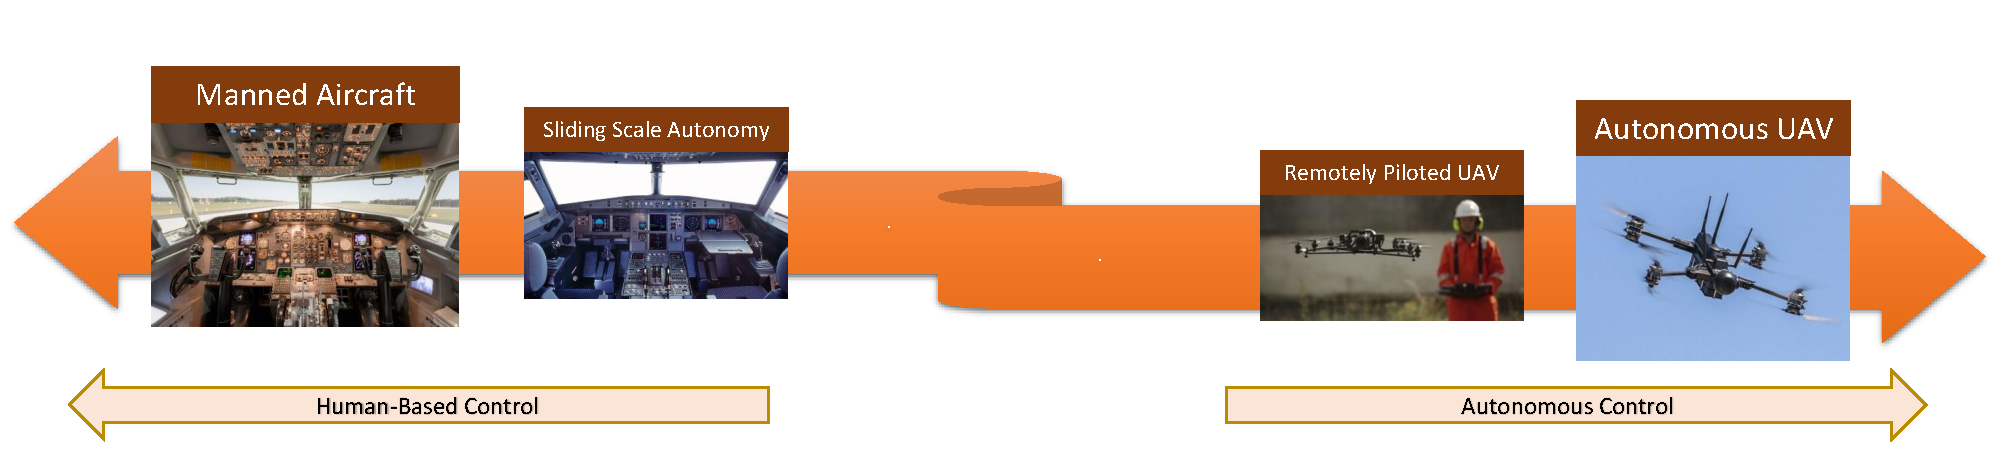
\includegraphics[width=6in]{overview}
\caption{Evolution of aircraft control from human to autonomy.}
\label{overview}
\end{figure}
Figure 1 depicts a spectrum of flight categories, ranging from fully human-driven to fully autonomous. This includes some intermediate categories such as sliding scale autonomy \cite{paras} to aid human pilots with a select amount of automated control or remotely piloted UAVs that involve both remote human control and some levels of autonomy. The overall scope of this research, however, focuses primarily on the two edges of the spectrum.

\section{Flight Performance and Safety}

Over the entire lifespan on manned aircraft, safety culture \cite{gibbons, boschert, remawi} has been a critical and overarching necessity throughout every facet of the design and planning of commercial and noncommercial flights, often serving as an important factor in customers' perception of flight safety \cite{brown, chang}. Despite this priority, a significant challenge lies within the ability of a crew member to effectively manage a high level of mental workload. This is primarily prevalent under pilots and air traffic controllers who work with enormous amounts of stress and multitasking. This results in a high amount of cognitive workload, which adversely affects an individual's situational awareness as well as one's ability to perform all given tasks effectively. In recent years, increases in partial autonomy have been introduced to ease a pilot's workload \cite{sherman}. 

The underlying challenge, however, lies within seamlessly transitioning between human control and autonomous control for a particular task in order to avoid counter-productivity caused by excess complexity and lack of understanding of the automation \cite{rudisill}, which could in turn lead to increased cognitive load from the autonomy itself \cite{funk}. For this, it is beneficial to detect and predict an individual's cognitive load in order to achieve early detection of cognitive overload (e.g.~a pilot is overwhelmed with too many tasks requiring significant amounts of precision) or underload (e.g.~so little is happening that a pilot's senses are dulled and he or she cannot respond as quickly to sudden changes of events). 

In predicting cognitive workload, many research efforts have sought to model cognitive workload using physiological and objective input data. These include many established machine learning techniques, such as artificial neural networks, support vector machines, and decision trees. By training any of these algorithms with appropriate data, early detection of cognitive workload levels can be utilized to seamlessly assist a human pilot or other crew member with intense levels of airline-related stress and multitasking.

\subsection{From Human Pilots to Autonomous Pilots}

As for unmanned aircraft, the challenges of human operators and cognitive workload are still prevalent, particularly when coordinating multiple UAVs simulatneously \cite{halverson}. However, a more recent trend in autonomous UAVs indicates a need to predict partly \cite{williams} or even fully \cite{albaker} autonomous behavior. By working to minimize the discrepancies between predicted behavior (e.g.~trajectories, actions, response to obstacles or other UAVs), these vehicles can benefit from improved safety, particularly due to the growing need for a standardized shared airspace \cite{nasem, albaker, hobbs, mccarley} that places UAVs into a similar frame of safety as those of manned aircraft. 

As in the case of manned aircraft, accurate modeling of input and output data can assist in effectively predicting future UAV behavior. By enhancing the accuracy of these predictions, pilots and mission planners can have a clearer idea of what is needed for a UAV to safely and successfully complete any mission objectives. In such cases, however, machine learning alone is not always enough to accurately model complex behavior, especially when many different types of data are involved. Hence, the concept of data fusion becomes one of great importance. Thus, by strategically applying both machine learning and data fusion, autonomous UAV behavior can be modeled in a way that are there fewer surprises and deviations between expectations and outcomes, thereby maximizing unmanned flight safety in increasingly complex mission scenarios.

\section{Motivations}

Placing focus on both manned and unmanned flight safety helps to identify and address the similarities that exist between the two types of aviation. Figure 2 provides a brief comparison of the challenges involved in both areas.
\begin{figure}[!t]
\centering
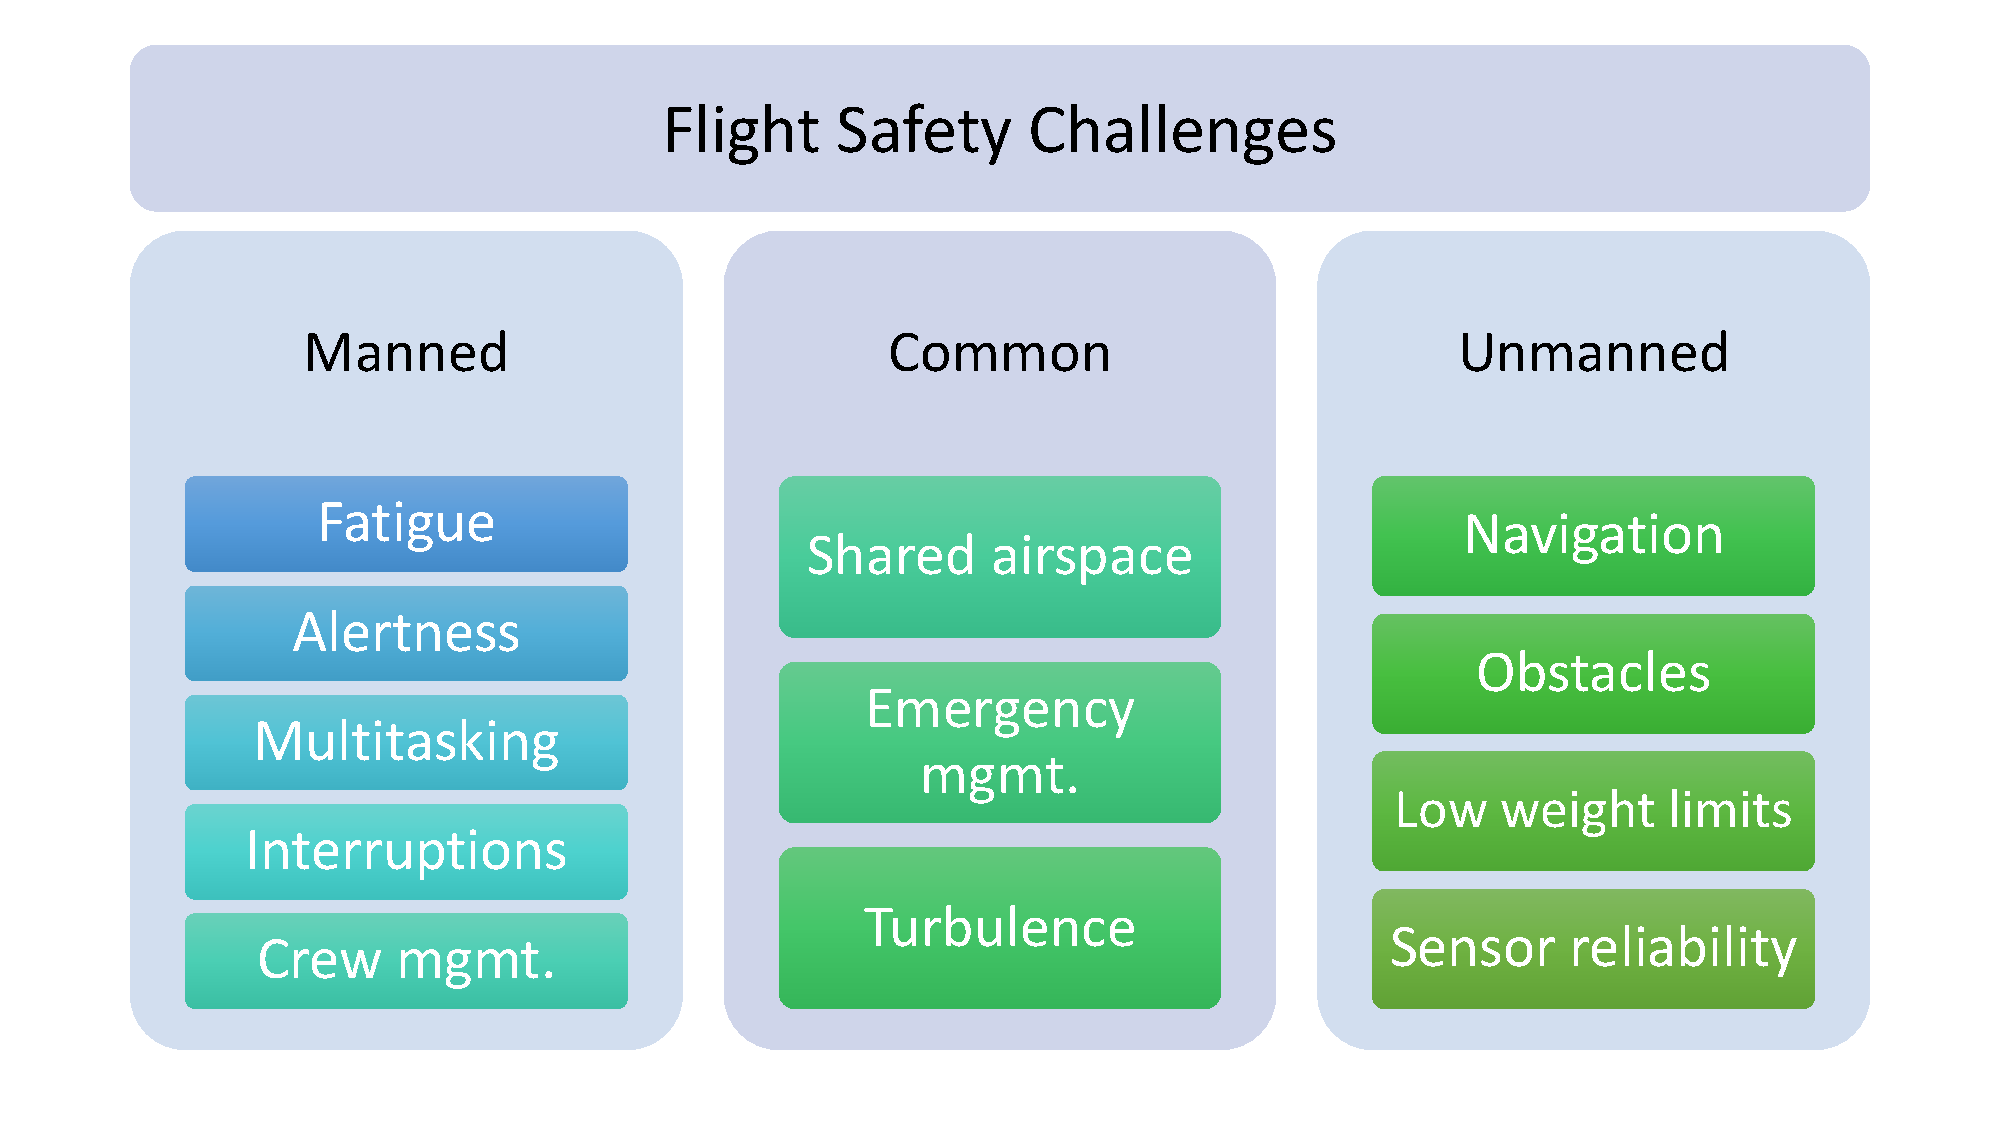
\includegraphics[width=6in]{challenges}
\caption{Comparison of flight safety challenges for manned and unmanned aircraft.}
\label{challenges}
\end{figure}
As their differences indicate, the challenges of manned aircraft are based primarily on human factors, such as fatigue, alertness, and crew management. Most of the unmanned challenges, however, are based on the UAV itself, including low weight limits, obstacles, and reliability of sensors \cite{hardin}. The abundance of shared challenges, however, including the issues of a shared airspace and emergency management, serve as the unified core of this research.

Most importantly, there are to date no current research publications that address manned and unmanned flight safety from a common lens. This observation is surprising given the above challenges and the technical milestones that have been applied to each from the perspective of machine learning. That is, given some kind of flight data, whether physiological from a pilot or sensory from an autonomous entity, this form of data science has played a crucial role in making predictions, classifications, and analysis on the state of either form of flight safety.

Thus, given such a background, this research aims to confirm that the use of machine learning can effectively aid in both focus areas in the predictions of relevant outcomes (e.g.~decreasing a pilot's cognitive workload, altering the intended trajectory of a UAV), which in turn can be uniquely assessed to improve flight safety.

\section{Research Objectives}

To thoroughly and effectively address both sides of flight safety improvement, this research proposes the following process:
\begin{itemize}
\item Identify different machine learning techniques used in assessing cognitive workload and test them on multiple physiological datasets to properly correlate physiological and objective inputs with different mental activities of varying cognitive load
\item Perform an analysis of alternatives on the different techniques based on the variety of results to determine the pros and cons of one algorithm over another under different scenarios
\item Develop a technique that dynamically chooses a machine learning algorithm based on the attributes of a given dataset and can change such an algorithm at different points of time if needed
\item Apply this novel technique in a way that it can alert pilots of potential future overload or underload, at which point steps can be taken to prevent such an imbalance, thereby improving human-side flight safety
\item Examine the effects of different machine learning techniques on autonomous UAV data and incorporate data fusion to combine multiple types of dissimilar data and improve prediction accuracy
\item Develop a technique that dynamically selects a prediction algorithm based on potential prediction accuracy and can switch methods over time when potential accuracy crossovers occur
\item Apply this technique on UAV data to ensure smoother autonomous path planning and behavior, thereby improving unmanned flight safety
\end{itemize}
By achieving these goals, greater improvements in aviation safety can be achieved in order to overcome many of the shared challenges on the manned and unmanned sides as well as their own unique challenges. 

\section{Publications and Contributions to Dissertation}

\begin{table}[!t]
\renewcommand{\arraystretch}{1.3}
\caption{Publications and contributions to dissertation.}
\label{publications}
\centering
%\resizebox{\textwidth}{!}
{\begin{tabular}{L{3.5cm} L{9.5cm}}
\toprule
Type & Publication/Contribution \\ \midrule
Journal Paper & Computational approaches for optimal manned and unmanned flight safety: a survey. \\
Conference Paper & Fundamental cognitive workload assessment: a machine learning comparative approach. \\
Conference Paper & Analysis of alternatives for neural network training techniques in assessing cognitive workload. \\
Journal Paper & Analysis of alternatives for machine learning in assessing cognitive workload. \\
Conference Paper & Adaptive machine learning approach for assessing cognitive workload. \\
Journal Paper & Enhancing human-driven flight safety through early detection of cognitive overload. \\
Journal Paper & Prediction of unmanned aerial vehicle behavior through a combination of Dempster-Shafer and artificial neural network sensor fusion. \\
Conference Paper & Adaptive machine learning system for enhanced UAV path prediction. \\
Journal Paper & Improving unmanned flight safety through adaptive machine learning of trajectory estimation. \\
Source Code & A re-usable Python library containing the source code of the algorithmic implementations for the manned phase of the research. \\ 
Source Code & A re-usable MATLAB library containing the source code of the algorithmic implementations for the unmanned phase of the research. \\ 
\bottomrule
\end{tabular}}
\end{table}

The major publications and contributions to this research are presented in Table \ref{publications}.

\section{Dissertation Organization}

This dissertation unfolds as follows:

Chapter 2 comprises the literature review of the dissertation. It provides a more in-depth look at past and present practices and challenges associated with flight safety. Also included are established uses of machine learning in cognitive workload assessment as well as their applications, the growing role of autonomy in flight, and established computational approaches for UAV data prediction.

Chapter 3 provides a theoretical overview of machine learning techniques relevant to cognitive workload assessment, a description and analysis of the relevant physiological datasets used in this end of the research, a thorough look at the results under numerous dimensions of variability, and a cost-benefit analysis of the different techniques under different conditions.  

Chapter 4 describes the premise and goals for implementing the previous techniques into an adaptive system. Also included are an algorithmic overview, results, discussion, and the resulting implications for the future of manned flight safety.

Chapter 5 contains the motivations for seeking enhanced UAV data prediction, an overview of the data fusion process, a description of the established competing techniques that are to be utilized for comparison, thorough results under the many dimensions of variability, and meaningful discussion.

Chapter 6 details the premise and goals for implementing the previous techniques into an adaptive system (similarly to Chapter 4 but for unmanned flight), an algorithmic overview, results under most of the same dimensions of variability, discussion, and implications for the future of unmanned flight safety.

Chapter 7 draws final conclusive remarks and discusses potential future ambitions in which this research could take shape.

Finally, this dissertation ends with an appendix, providing instructions on how to obtain any or all of the project source code.

% Chapter 2

\chapter{Computational Approaches for Optimal Manned and Unmanned Flight Safety} 

This chapter consists of a comprehensive literature review. This includes general flight safety practices and challenges, the evolution from human control to autonomy, an overview of cognitive workload in manned and unmanned aircraft, established roles of machine learning in workload assessment, autonomy in flight, and methods for assessing autonomy. A key observation is that in examining prior research on flight safety, a wide variety of prior works exist on both the manned and unmanned sides, but none appear to examine both areas together. The findings and analyses of the literature in these areas serve as the bases for the many technical phases of this dissertation.

\section{Flight Safety Practices and Challenges}

The concept of flight safety itself is a topic that has been prominent in literature for decades that has been approached from a variety of angles. For instance, Campbell and Lahey wrote a survey in 1984 that details aircraft accidents that resulted from fatigue failures in aircraft \cite{campbell}. More specifically, these accidents are the result of hardware failure in various parts of the aircraft that can be resolved by design, testing, load monitoring, inspection, and part replacements in that order. In 1990, a publication by Wycoff and Holley examined the effects of pasengers' perception of an airline and its flight safety based on being touched on the shoulder or forearm by a flight attendant \cite{wycoff}. In a more general context, O'Hare and Chalmers published a 1999 study comparing accident rates from multiple parameters, including categories of aircraft and hazardous conditions such as low fuel \cite{ohare}. Other works include a 2001 link between safety attitudes with flight performance \cite{sexton}, the proposal of a new safety index in 2004 based on relative safety level from the perspective of risk and competitive safety \cite{chang2}, and improvement of flight safety based on prediction of bird migration patterns \cite{vanbelle} in 2007. A 2009 work by Macrae oversaw a need for improved risk management by increasing the visbility of potential threats \cite{macrae}. By 2011, thorough reviews of measuring aviation safety climate from a wide range of variables are more prominent \cite{oconnor}. 

Overall, a key limitation in human-driven flight is the general concept of human error \cite{dhillon,kirwan,kirwan2}. One such cause of error is pilot fatigue \cite{conway,caldwell,rosekind10}. This can be caused by a variety of factors, such as regional airline operations (e.g.~regulatory differences, scheduling practices) \cite{rosekind11}, long haul flight operations (e.g.~rapid time zone changes, sleep disturbances) \cite{rosekind12}, and corporate flight operations (e.g.~unscheduled flights, extended duty days) \cite{rosekind13}. Other key drivers are the attitudes and safety cultures of a flight crew \cite{sexton, remawi} as well as weather-related issues \cite{emo}. Overall, these limitations can lead to reduced task engagement \cite{matthews}, slower movement, increased mistakes, and memory difficulties \cite{caldwell} as well as general confusion and cognitive impairment \cite{west}. Another key deficiency is the effect of concurrent task demands \cite{louk}, or the need to run multiple tasks at the same time that are frequently interrupted.

It should also be noted that pilots are not the only members of the flight crew that endure large amounts of stress. Other humans affected include air traffic controllers \cite{mfunke,duley,abbass,chatterji,brookings,gianazza} and even flight attendants \cite{kelleher}. 

\section{Optimizing Human Control through Cognitive Workload Assessment}

The ability to effectively manage a pilot's mental workload under periods of stress \cite{sanders, hockey, mendl}, fatigue, and high levels of multitasking is key to ensuring successful human performance. Thus, the ability to make classifications, predictions, and assessments of cognitive workload in essential applications remains an ongoing research challenge. More recently, a variety of machine learning algorithms have become available that address cognitive workload assessment quite well. These range from support vector machines and decision trees to k-nearest neighbors and artificial neural networks.

\subsection{Cognitive Workload}

\begin{figure}[!t]
\centering
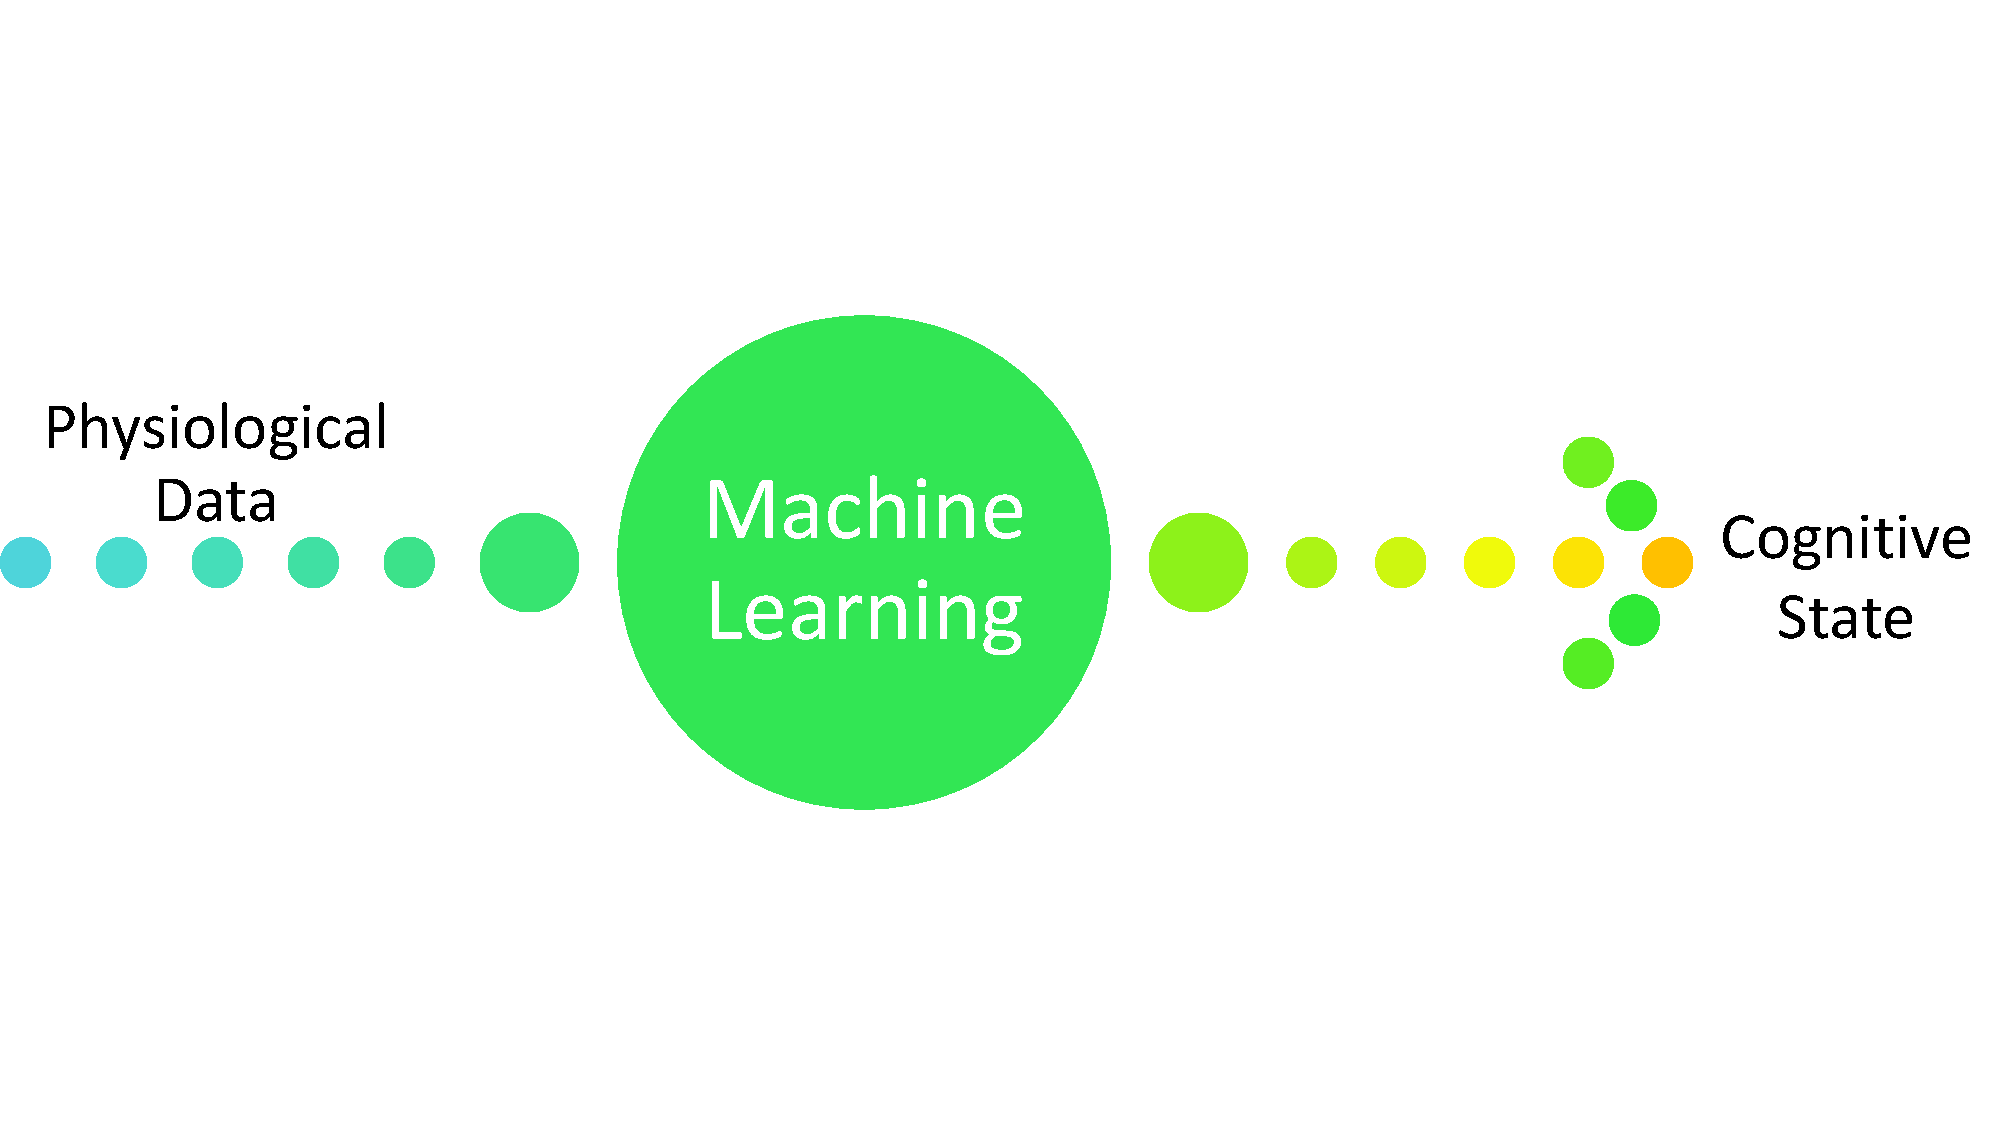
\includegraphics[width=6in]{cw}
\caption{Role of machine learning in the assessment of cognitive workload.}
\label{challenges}
\end{figure}

Cognitive workload refers to the overall amount of effort being utilized in working memory. In a certain light, the concept can be regarded as a type of balancing act between underload and overload of such memory. For instance, many prior human factors research efforts have sought to address the problem of overload \cite{berka}, such as when an individual is given tasks that are too numerous or too difficult, making one's overall performance of such work less than optimal. 

Based on prior research efforts, detection and prevention of mental overload appear to be the more established objectives, particularly in applications such as general cognitive tests \cite{berka}, piloting of remotely operated vehicles \cite{durantin}, science education \cite{niaz}, team-based command and control environments \cite{gfunke}, and even ordinary driving \cite{lenn,reimer,collet}. Overload generally occurs when one must undergo numerous parallel tasks and/or difficult tasks, which results in increased human error. 

Conversely, however, the possibility of underload \cite{dillard} must also be addressed. For instance, a traveler engaging in a long and monotonous drive may in fact benefit from increasing mental workload, as a low amount may find the driver in a ``highway hypnosis,'' dulling his senses and leaving him unable to react effectively to sudden changes, such as the immediate slowdown of a leading car.

Overall, the ability to accurately and effectively assess one's cognitive state has remained a vital challenge in the field of neuroergonomics. Furthermore, the desire to predict, classify, and otherwise manipulate cognitive workload assessment has been greatly aided by the many novel facets of machine learning.

\subsection{Machine Learning}

Machine learning is a broad and well-recognized research field that spans across a wide variety of applications. Cognitive workload is no exception and has been addressed by this field in a vast plethora of ways.

Like with any machine learning problem, the key to forming an accurate and effective model is to properly decide the relevant inputs and outputs. Inputs in this field are typically physiological in nature and have included heart rate \cite{strang,henel}, respiratory \cite{wilson}, electrocardiographic (ECG) \cite{wilson,dussault}, eye movement \cite{halverson}, near-infrared spectroscopy (fNIR) \cite{hincks,cakir}, magnetoencephalographic \cite{kramer}, and electroencephalogram (EEG) \cite{berka,christen2,gfunke2,bashivan} data, the latter of which seems to be the most common \cite{wilson, zheng, bashivan}. Electrodermal activity (EDA) also appears to be a promising physiological input in cognitive activity \cite{natarajan}. In the context of pilot workload, heart rate, heart rate variability, blood pressure, and respiration are common physiological metrics \cite{veltman,roscoe,lee}.

% add figure from PPT of Supervised/unsupervised methods 

\begin{figure}[!t]
\centering
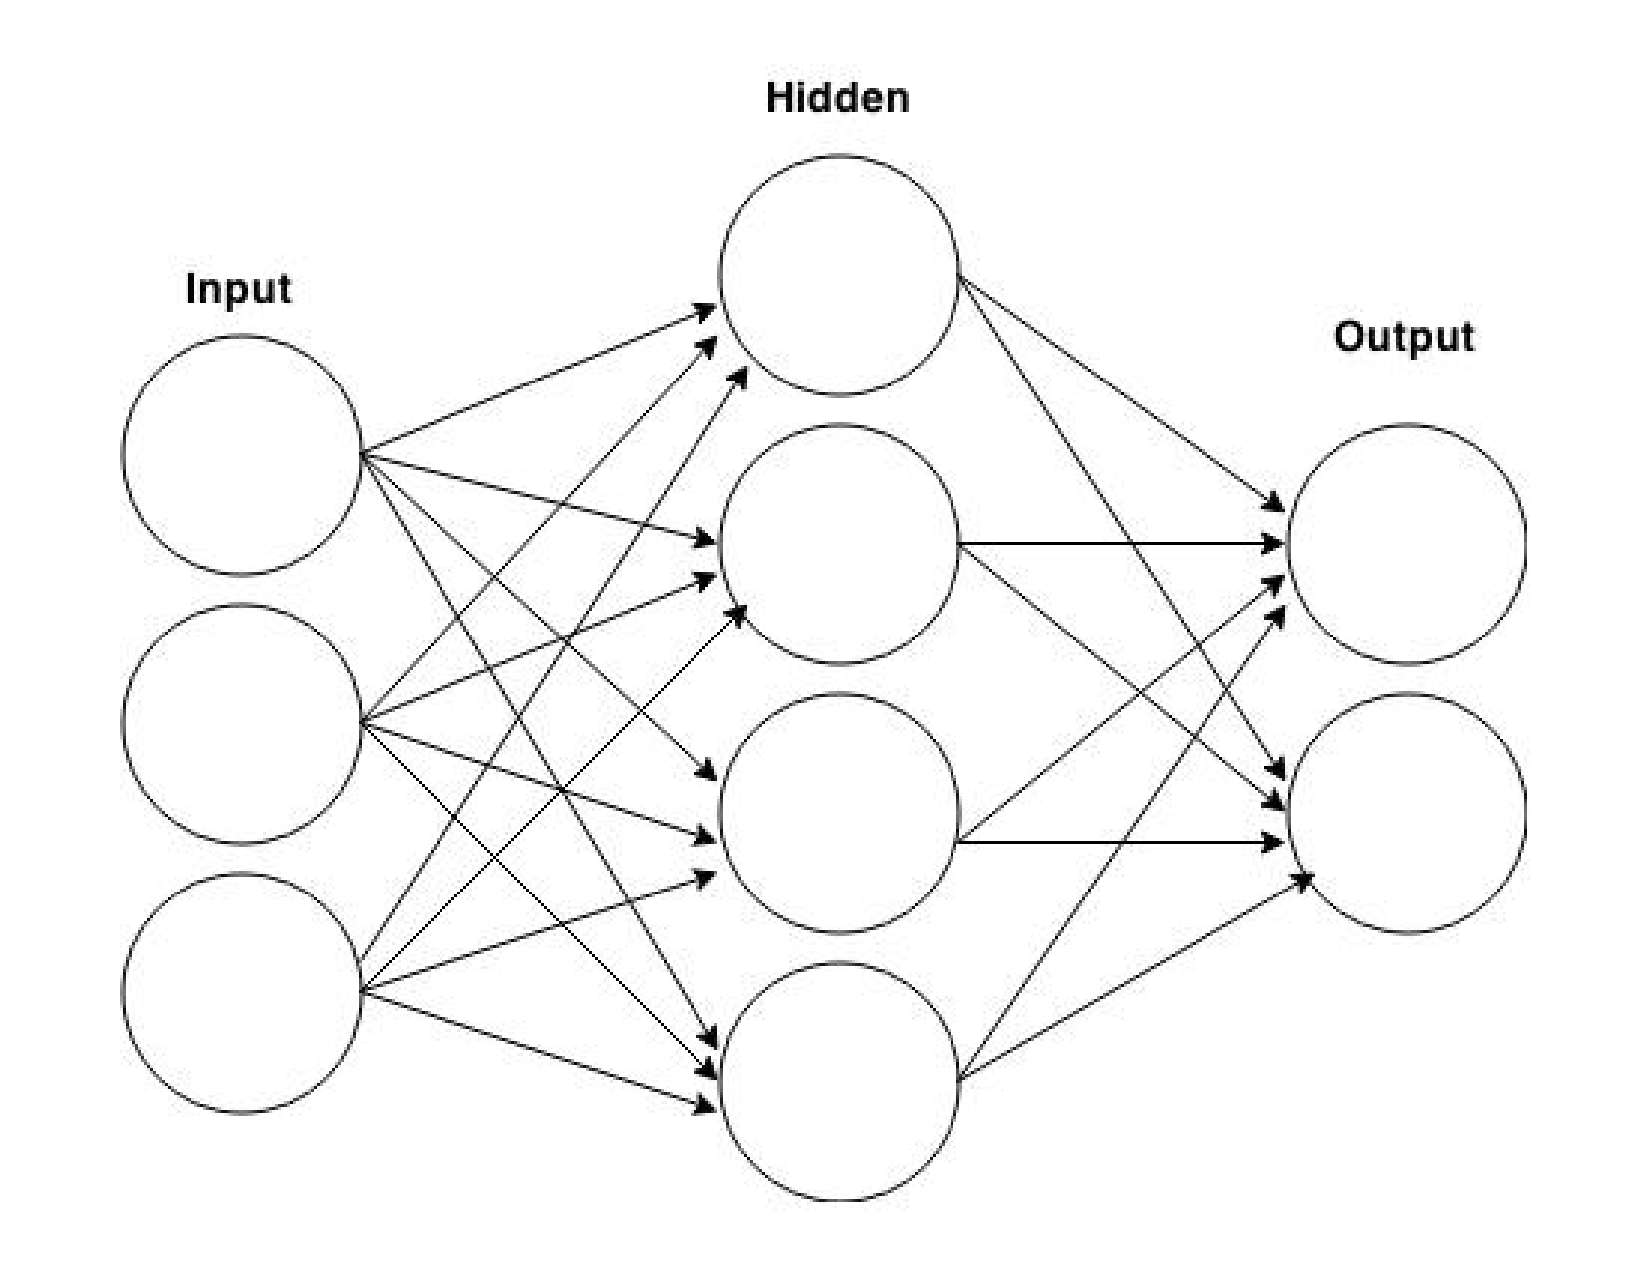
\includegraphics[width=6in]{ann1}
\caption{Overview of an artificial neural network.}
\label{challenges}
\end{figure}

\subsubsection{Artificial Neural Networks}

An artificial neural network (ANN) is a common machine learning algorithm based on biological neural networks. Many types of supervised ANNs, such as multilayer perceptron (MLP), consist of multiple layers of nodes. In the case of MLP, these neural networks consist of input, output, and hidden nodes \cite{malsburg}. 

The multilayer perceptron (MLP) feed forward equations are \cite{mavr}
\begin{equation}
y_k = v_{0k} + \sum\limits_{j=1}^{n_h} v_{jk} z_j
\label{eq1}
\end{equation}
and
\begin{equation}
\gamma_j = u_{0j} + \sum\limits_{i=0}^{n_i} u_{ij} x_i,
\label{eq2}
\end{equation}
where $k=1,2,\dots,n_o$ in Equation~\ref{eq1} and $j=1,2,\dots,n_h$ in Equation~\ref{eq2}. ${n_i}$, ${n_h}$, and ${n_o}$ are the numbers of input, hidden, and output neurons, respectively. Furthermore, all ${x_i}$ values are based on given input values in a particular sample of data, and ${z_j}$ is based on the sigmoid activation function
\begin{equation}
z_j = \frac{1}{1+e^{-\gamma_j}}.
\label{eq3}
\end{equation}
Once the neural network architecture, i.e.~set of weights and biases, is decided, the weights are initialized while the model output is calculated. These variables can be trained using supervised techniques such as quasi-Newton, stochastic gradient descent, or the limited-memory Broyden–Fletcher–Goldfarb–Shanno (L-BFGS) algorithm.

ANNs appear to be most established in a variety of cognitive workload problems, including classification of mental workload \cite{wilson,wilson2,wilson3}, qualitative analysis based on air traffic data \cite{chatterji}, cross-task workload \cite{wilson, baldwin}, and classification of crewmember workload \cite{laine}. A subset of ANNs known as deep neural networks (DNNs) has been applied to similar but differing applications, such as emotion recognition \cite{zheng}, brain-computer interfaces \cite{hennrich}, and analysis of human activity \cite{sarkar}.

In supervised ANNs, two of the most established optimization methods include quasi-Newton and stochastic gradient descent. Regarding cognitive load, the latter training technique has modeled temporal dependencies using memory structures \cite{hefron} and workload model performance \cite{gianazza}, while the former aided in inferring mental load based on pupillary dilation \cite{juhaniak} and both methods served as classifiers in decision support sys-tems \cite{tran}. It is worth noting that only some of these applications have used these optimizers specifically for ANNs while others have utilized these as standalone numerical methods. Other training methods include global techniques such as ant colony optimization \cite{mavr}, in which a biologically inspired technique is based on the behavior of ants. For unsupervised ANNs, restricted Boltzmann machines have found success in assessing cognitive workload across multiple tasks \cite{ziegler}. Relative to assessing pilot workload, ANNs have been used in evaluation within a flight simulator based on ECG measurements \cite{hannula}.

\subsubsection{Support Vector Machines}

Support vector machines (SVMs) are a two-group classification problem that maps data points onto a high dimensional space \cite{cortes}. In this technique, a support vector network maps multiple input factors into such a space through nonlinear mapping techniques \cite{cortes}. The term support vector refers to the vectors that determine the largest margin of separation between two groups. In general, SVMs offer fast training in a distributed manner with efficient use of processing resources. Due to the relatedly binary nature of SVM outputs, this technique is more beneficial when a problem seeks qualitative outputs rather than quantitative ones. Common parameters include the penalty term, the kernel type (such as linear or radial basis function), and gamma value (also known as a kernel coefficient). SVMs are well-known for assessing the cognitive state of a driver \cite{jin, son, putze, liang} and addressing mental workload from a more general context \cite{ziegler, yin}. Classification of driver workload has also succeeded under decision trees (DTs) and k-nearest neighbors (KNNs) \cite{solovey}.

\subsubsection{K-Nearest Neighbors}

K-nearest neighbors (KNN) is a classification technique that seeks a majority point from $k$ neighbors of a data point in space. In the case of binary classification under the label set $\{0,1\}$, KNN can be defined as \cite{kramer2}
\begin{equation}
f_{KNN}(x') = \begin{cases}
	1, & \sum_{i \in N_K(x')} y_i \geq 0 \\
	0, & \sum_{i \in N_K(x')} y_i < 0
	\end{cases},
\end{equation}
where $K$ is the neighborhood and $N_K(x')$ is the set of indices of the K-nearest patterns. In non-binary classification, the function can be rewritten as
\begin{equation}
f_{KNN}(x') = \arg\max_{y \in y} \sum_{i \in N_K(x')} I(y_i = y),
\end{equation}
where $I(\cdot)$ is an indicator function that returns one if true and zero if false. Weights can be either uniform or inversely proportional to the distance from a point of interest. Other parameters include leaf size and number of neighbors. Some relevant KNN applications include cognitive stress recognition \cite{calibo} and brain-computer interfaces \cite{girouard}.

\subsubsection{Decision Trees}

Decision trees (DTs) are a supervised learning technique that forms predictions and classifications based on decision rules established from the features of some given data \cite{breiman}. It is based on the pre-computational concept of a decision tree, which is essentially a flowchart in which every non-terminating block is a question with two possible paths. Some DT parameters include the minimum samples needed to split a node or exist at a leaf node as well as the criterion for measuring a leaf split's quality. DTs are useful due to the ease of data preparation and visualization but function at the expense of possible overfitting and unbalanced data. 

\subsubsection{Random Forest}

Random forest (RF) is a type of ensemble method, that is, one that aggregates multiple classifiers. As the name forest suggests, it is an ensemble of decision trees in which some trees are given extra weight to incorrectly predicted data points \cite{liaw}. This type of averaging helps in improving accuracy and reducing the possibility of overfitting.

\section{From Human Control to Autonomy}

In recent years, autonomy has aided in easing cognitive workload \cite{endsley,rudisill}. From there, the challenge lies within applying a seamless blend of human and autonomous control based on the needs of one's mental load. The concept of sliding scale autonomy has greatly aided in this effort, in which a variable amount of autonomy can be adjusted at any given moment \cite{bruemmer, desai}. In addition to adjusting between various levels seamlessly, the issues of trust \cite{helldin} and adaptability \cite{christen} between human and autonomy must also be taken into consideration as well as deciding an appropriate amount of interaction \cite{beer}. Meanwhile, the field of unmanned aerial vehicles (UAVs) poses its own unique challenges of integrating into a shared airspace \cite{parke,chevalley,rein}. 

Most established UAV applications are primarily under remote human-centric control \cite{kirwan,kirwan2,dhillon,kurk,peschel}, which require many human factor considerations similarly to manned aircraft \cite{guznov,cooke,jasper,chen2,wohleber}, especially when piloting multiple UAVs simultaneously \cite{lin}. However, recent research has led to the expansion of fully autonomous control \cite{clough,karim,tomic,burkle,valavanis,bosch} in a variety of applications, such as search and rescue \cite{fabiani} and 3D mapping \cite{nex}. From here, minimizing discrepancies between predicted UAV behavior and actual outcomes is an ongoing task to ensure a safe and reliable flight. Prior solutions include the use of machine learning techniques similarly to those in Subsection 2.2.2. Other approaches involve the use of cognitive architectures \cite{franklin} such as Soar \cite{laird, nuxoll} and ACT-R \cite{anderson}.

\section{UAV Autonomy in Flight}

In recent years, unmanned aerial vehicles (UAVs) have become a dominant force in military operations as well as in commercial and recreational applications.
UAVs can be controlled either manually via a remote pilot or autonomously.
Either case presents numerous degrees of variability and unpredictability due to the behavior of the human pilot or autonomous system and can adversely affect team performance \cite{salas}, leading to the necessity of blame assignment \cite{malle}.
Thus, creating a mechanism for explaining the behavior and decisions of autonomous UAVs is of particular interest, due to the novel factors that comprise such an explanation. 
These can include memory-based data structures, memory reconstruction, explanation algorithms, and explanation interfaces.

Episodic memory is a valuable tool that can substantially aid in many of these factors \cite{tecuci}. It is a type of memory in which past experiences or events can be remembered explicitly \cite{wang, stach, subaj, jockel, wang2, wang4}, such as remembering a name and circumstances of a specific interaction \cite{wood}. From here, an autonomous agent can learn from past experiences \cite{kelley}.
It is particularly useful due to the ability to determine a quality of interestingness in intelligent agents \cite{kadlec,macedo,macedo2,macedo3,nuxoll} as well as in other applications such as image processing \cite{chu,derbinsky}, emotional intelligence for intelligent agents \cite{kazem}, or modeling of autobiographical memory \cite{wang3,barakova}.
In a simplified context, interestingness can be expressed as a significant difference between a predicted result and an actual result.
While correlating and predicting decisions based on sensory data \cite{javaid} is already a fundamental and well-established concept, doing so in the context of finding interestingness to explain UAV behavior forms a new realm of possibilities.

\section{Computational Approaches to UAV Data Prediction}

Prediction of UAV-based attributes is presently a well-established field spanning a wide array of applications. 
Over the past two decades, these applications have steadily shifted from human-centered manual control to self-contained autonomy.
For instance, under the early stages of manual UAV control, research efforts involved the assessment and prediction of human performance, such as using quantitative models for predictions regarding multi-UAV flight control \cite{dixon}.
Eventually, this evolved into a more supervisory role, with limited amounts of UAV autonomy used to reduce human workload \cite{cummings}.
Thus, prediction focused on cognitive capacity based on factors such as wait times and situational awareness.

Other early works in UAV prediction stemmed from a focus on control systems, often using common machine learning techniques to aid in a vehicle's control system.
One such effort involves the development of an output feedback controller based on neural networks \cite{dierks}.
Controller design was improved years later as support vector regression was proposed as a direct alternative for the kinds of dynamic control systems needed for a UAV \cite{shin}.
The focus on control is also present in more non-traditional UAV applications, such as in modeling a vehicle to perch on a wire in a manner similar to that of a bird for the purpose of evading attacks \cite{hoburg}.
Accomplishing such a task requires a significant amount of creativity regarding aerodynamic modeling and design of an effective control system, which was met through physically-based basis functions for attributes such as position, velocity, and angle.

In addition, machine learning approaches have been used in a variety of additional UAV-related fields. 
This includes applications based on drone images, such as tree detection from LiDAR data through a variety of algorithms \cite{wallace}, classification of informal settlements from 2D and 3D features via feature extraction \cite{gevaert}, and traffic monitoring from video data by statistical profile generation \cite{puri}. Engine fault prediction is another area, leveraging particle filters to predict needs and urgency for system maintenance \cite{baoan}.

Because the portion of this research focused on unmanned flight safety involves location and navigation, it is appropriate to consider a major amount of related work in these two areas. 
Previous efforts regarding prediction of individual navigation-based attributes such as altitude or speed have in at least some capacity spanned as far back as initial stages of UAV research.
An early example includes the assessment of a UAV's situational awareness, or more specifically the ability to autonomously monitor an object of interest based only on its trajectory \cite{jaen}.
This was accomplished through modeling of physics based differential equations as a form of state estimation.
Later work involved estimating location-based qualities of the UAVs themselves, such as prediction of altitude based on a single integrated camera and a semi-supervised machine learning approach \cite{cherian}. 
Other predictions included a UAV's heading and external wind conditions using time integration of inertial navigation system data \cite{rhudy} as well as estimation of a vehicle's mobility in the context of an ad hoc UAV network \cite{lin}.

Using prediction for the purpose of forming entire paths is a logical next step, and prior works have addressed this manner quite extensively.
These consist of basic localization problems, such as estimating a location based on digital elevation map data and infrared images. 
This was done in order to aid UAV navigation in mountainous and dark terrains in which charge-coupled device (CCD) camera data are ineffective \cite{woo}.
Other approaches focus on path planning, including a waypoint-based design to minimize location uncertainty \cite{dogan} as well as a multi-UAV approach based on data fusion for a security-focused application of intelligence, surveillance, and reconnaissance \cite{shen}.
Trajectory tracking is another method, originally used in situational awareness \cite{cummings} by tracking objects relevant to a UAV. 
This evolved into adaptive trajectory tracking for aiding in UAV guidance \cite{wang6}.
Collision avoidance is another vital aspect of navigation, developments of which have been based on factors such as visual detection \cite{zsed} and flight space geometry \cite{wang5}.

\subsection{Sensor Fusion}
\label{sensor}

Sensor fusion, or the ability to fuse dissimilar data to enhance algorithmic effectiveness, has been relatively commonplace in navigational applications. 
For instance, many algorithms have sought to fuse global positioning system (GPS) and inertial navigation system (INS) data to solve the problem of GPS outages in critical military and civilian applications \cite{rhudy2, adus, bhatt, adus2, aggarwal, bhatt2}. 
This type of information fusion has also made its way to UAV navigation \cite{nemra, yoo}.
Other relevant uses for sensor fusion have been found in more mission-specific applications, including command and control systems \cite{verma}, situational awareness \cite{chen}, and target identification \cite{yu2}. 
Efforts in UAV navigation research have also improved under data fusion \cite{rhudy, shen} as well as applications in engine diagnostics \cite{basir, safiz} and sensing networks \cite{whyte}.

\subsection{Neural Network Data Fusion}
\label{ann-fusion}

While artificial neural networks are not explicitly a form of data fusion, many previous research efforts have successfully implemented ANNs alongside different data fusion techniques to address a wide variety of applications. 
For instance, \cite{chen2} addressed multiple methods of fusion in tool condition monitoring. 
In this approach, sensor fusion aided in integrating feature elements, which were then trained by an ANN.
The combination of tool condition monitoring, data fusion, and neural networks has been surprisingly common and has shown up in many different works over the past 30 years \cite{chen2, ghosh, dornfield}.
Similar applications have included fault diagnosis for manufacturing systems \cite{yuqin} and water quality estimation \cite{zhang}, while less similar fields have involved cloud analysis \cite{loyola}, smart cars \cite{nelson}, and multitemporal change analysis \cite{dai}.
Regarding specific data fusion approaches, both Bayesian Inference \cite{li} and Dempster-Shafer evidence Theory \cite{deno} have been integrated with ANNs.
When considering relevance to the application of this paper, there has been work in applying ANN data fusion to target tracking \cite{chin} and localization of mobile users \cite{meri}.
More relevant areas, such as estimating the location or path of a UAV, has not yet been addressed by neural network data fusion.


\subsection{Dempster-Shafer Evidence Theory}
\label{dset}

Dempster-Shafer Evidence Theory (DSET) is a unique data fusion technique based on Bayesian combinational probability that approaches the concept of combinational factors in a distinctly different direction \cite{nguyen}. 
While Bayesian statistics utilize combinations of internal probability factors within a system \cite{chiodo}, typically by use of random variables or propositions, DSET dynamically involves external evidence factors \cite{limbourg, lipeng} to make decisions or predict values. 
Each factor contains a data range in which a potential output value can lie as well as a confidence probability that the data range is reliable, or certain. 
DSET is meant to model information that, under more traditional Bayesian methods, would be considered incomplete \cite{nguyen}. 

\subsubsection{Bayesian Origins} 

Bayesian probability is a technique in which two or more internal probabilistic factors are combined to form a single hypothesis or inference, often using random variables to fulfil unknown quantities in the context of a problem \cite{rish}. If only two factors, $X$ and $Y$, are considered, then Bayesian inference can be defined as
\begin{equation}
P(Y|X)=\frac{P(X|Y)P(Y)}{P(X)},
\label{bayes1}
\end{equation}
where $P(X|Y)$ denotes the probability of event $Y$ occurring given event $X$, $P(Y)$ represents the probability of $Y$ alone, $P(X)$ is the probability of $X$ individually, and $P(Y|X)$ is the probability of $X$ given $Y$. 

Bayesian estimation has been established in a variety of applications, including wind speed probability distribution \cite{chiodo1} and battery lifetime analysis \cite{chiodo2}. 

\subsubsection{Theoretical Foundation}

From a theoretical context, Dempster-Shafer Evidence Theory can be best described as a generalization of Bayesian probability theory, forming a divergence based on the concept of ignorance. Typical Bayesian approaches assume an ignorance quantity of zero, or equivalently 100\% confidence, for any probabilistic value, which is usually appropriate when a probability factor is internal. Because DSET is based on external factors, however, this property can no longer be unconditionally assumed, and thus a plethora of evidence factors are used to determine all possible outcomes in a given scenario, each with its own degree of confidence that serves as a weight of evidence \cite{shafer}. The finite set of all possible mutually exclusive values is known as the frame of discernment and is denoted by $\Theta$. From there, the union of all subsets is given by the power set $2^\Theta$.

One of the most significant fundamental concepts of DS Theory is the basic probability assignment (BPA) function, which is essentially the equivalent of the random variable in Bayesian probability theory and is also known as the belief variable \cite{auer}, denoted as $m$. Suppose $A_1,\dots,A_n$ are all possible sets within a frame of discernment, noting that $A_i \in 2^\Theta$. Then
\begin{equation}
m: 2^\Theta \rightarrow [0,1], \sum\limits_{i=1}^n m(A_i) = 1, m(\emptyset) = 0,
\label{init}
\end{equation}
\noindent where $\emptyset$ denotes the empty set. Each set $A_i$ takes the form of the interval $([\ubar{x},\bar{x}])$, denoting the lower and upper bounds of an evidence factor, respectively \cite{auer}. Each BPA $m$ consists of two vital properties: a range, as established by a set $A$, and a degree of confidence $\mu$ that lies within the range of [0,1] \cite{ipp}. Thus, ignorance can be defined as simply $1 - \mu$. At certain times, manually adding new BPAs can be an exhaustive process, in which case sampling from a distribution becomes an ideal solution. This process, also known as discretization, involves generating $n$ discrete samples based on a lesser amount of initialized BPAs, which collectively form a cumulative density function (CDF) of BPA structures \cite{tonon}.

Once two or more evidence factors from different sources exist in the same problem, then typically the aggregation of BPAs becomes essential \cite{auer}. Many possible methods exist in which this task can be accomplished, but the scope of this research focuses primarily on Dempster's rule of combination. Suppose $m_1$ and $m_2$ denote two BPA functions that are to be aggregated. Under Dempster's rule, a new BPA function $m_1 \oplus m_2 : 2^\Theta \rightarrow [0,1]$ is defined as \cite{alani}
\begin{equation}
[m_1 \oplus m_2] = \frac{\sum\nolimits_{A\cap B = y} m_1(A)m_2(B)}{1-\sum\nolimits_{A\cap B = y} m_1(A)m_2(B)}
\label{agg}
\end{equation}
\noindent on the condition that $y \neq 0$. Otherwise $[m_1 \oplus m_2] = 0$. 

Belief and Plausibility are two of the most vital core functions of an aggregate BPA, as they represent the best and worst case scenarios, respectively, in a frame of discernment and are defined as
\begin{equation}
Bel(B) = \sum\nolimits_{A_i \subset B} m(A_i)
\label{bel}
\end{equation}
and
\begin{equation}
Pl(B) = 1 - \sum\nolimits_{A_i \cap B = \emptyset} m(A_i),
\label{pl}
\end{equation}
\noindent where $m(A_i)$ denotes the BPA mass function for a set $A_i$.

Some applications that have incorporated DSET in the past include a variety of localization problems, such as in wireless sensor networks \cite{elkin}, robot localization \cite{clarentin}, and indoor localization of mobile users \cite{kaseb}. 
Other applications include image classification \cite{rotten} and detection of credit card fraud \cite{panigrahi}.
As previously mentioned, it has been implemented successfully in fusion of sensors for enhanced vehicular navigation \cite{bhatt, aggarwal}. However, this framework has not been implemented in UAV-based data prediction.

\subsection{Kalman Filters}

When discussing prior work involving UAV data prediction, an important class of algorithms is that of the Kalman filter. Kalman Filter is a type of parameter estimation in which mathematical models can be formed based on measured data \cite{chow}. It is based on a two-step Bayesian model of stochastic filtering that consists of prediction and correction. However, it has also been shown that these filters tend to underperform ANN-based solutions in related applications \cite{aydo}.

\subsubsection{Extended Kalman Filter}

The Extended Kalman Filter (EKF) is a variation that implements instantaneous linearization at each time step to approximate nonlinearities \cite{chow}. It is considered the most popular method of nonlinear filtering in the field of aerospace. More specifically, it has been applied in UAV localization \cite{mao} and trajectory prediction \cite{prevost}.

\subsubsection{Unscented Kalman Filter}

The Unscented Kalman filter (UKF) differs from EKF in that less linearization is involved \cite{chow}. Instead, it uses sample points to approximate a probability distribution. UKF is not quite as widely used as EKF in this area. However, it does have established roots in UAV navigation \cite{oh} and general parameter estimation \cite{chow}.

\chapter{Cognitive Workload Assessment}

In order to address human-side flight performance, the concept of cognitive workload becomes a subject of particular importance. This chapter details the portion of the dissertation research concerning the assessment of cognitive workload and bridges it with fundamental machine learning (ML) concepts. This includes a conceptual review of both cognitive load and its previous applications in machine learning as well as the details of the experimental procedure to compare and contrast various candidate ML techniques on multiple sets of cognitive data. Following thorough experimental results, an extensive cost-benefit analysis of the different fundamental methods is then discussed, followed by conclusions regarding ML's potential roles in human-oriented flight performance.

\section{Introduction}

As discussed in Chapter 2, cognitive workload is the amount of mental effort that is stored in working memory. It can be perceived as a balancing act between overload (e.g.~driving in downtown Chicago traffic while talking to passengers, using a smartphone, and listening to the radio) and underload (e.g.~driving on a rural highway with other no vehicles around, no passengers, and the radio turned off). In the field of flight safety, overload is typically the more common of the two extremes. The use of sliding scale autonomy is a common way to reduce a pilot's workload, while underload could be resolved with a simple alert. In these cases, it is useful to detect the potential of cognitive overload or underload as early as possible. Thus, machine learning can be applied to examine any non-invasive physiological data combined with current levels of cognitive load and thereby predict future load levels based on ongoing trends.

From there, the challenge is to identify which machine learning method is best. Many different techniques have been established in these kinds of applications, including artificial neural networks (ANNs) \cite{chatterji,gianazza,wilson,wilson2,wilson3,hefron,juhaniak}, support vector machines (SVMs) \cite{jin,son,putze,liang,ziegler,yin}, k-nearest neighbors (KNNs) \cite{solovey,calibo,girouard}, decision trees (DTs) \cite{solovey}, and random forests (RF) \cite{liaw}. Thus, this phase of the research consists of a twofold approach: compare and contrast the established techniques based on extensive experimental analysis, and develop an adaptive algorithm that dynamically selects a technique based on the attributes of some given physiological data. This chapter focuses on the former.

\begin{table}[!t]
\caption{Summary of cognitive workload datasets used in this experiment.}
\renewcommand{\arraystretch}{1.3}
\centering
\resizebox{\textwidth}{!}
{\begin{tabular}{*{4}{l}}
\toprule
ML Technique & Subjective Parameter & Iterative Parameter 1 & Iterative Parameter 2 \\ \midrule
Artificial neural network (ANN) & Training (SGD, LBGFS) & No. hidden layers & No. hidden neurons \\
K-nearest neighbors (KNN) & Weights (uniform, distance) & No. neighbors & Leaf size \\
Support vector machines (SVM) & Kernel (linear, RBF) & Penalty term & Gamma value \\
Decision tree & Criterion (gini, entropy) & Min. samples for split & Min. samples for leaf \\
Random forest & Criterion (gini, entropy) & Min. samples for split & Min. samples for leaf \\ \bottomrule
\end{tabular}}
\label{params}
\end{table}

When performing an analysis of alternatives, it is important to have as many relevant variables as can be reasonably accommodated. One of the most apparent is a quantity and variety of data. This chapter approaches data variability by starting with more generalized physiological data with a sufficient amount of relevance to cognitive workload, then evolving to a more specific dataset that directly involves pilots and flight safety. The remaining variables remain specific to the different machine learning techniques to be analyzed. These attributes can be subjective, such as ANN training method, SVM kernel, KNN weight considerations, and DT/RF criteria. They can also be more iterative in nature, such as the number hidden layers or hidden neurons in an ANN, penalty term and gamma value in a SVM, number of neighbors and leaf size in KNN, and minimum number of samples for split or leaf in DT and RF. Table \ref{params} provides an overview of the three method-specific parameters to be selected for each technique.

By analyzing all these candidate machine learning techniques under the aforementioned experimental parameters, the advantages and disadvantages of these methods under the context of assessing cognitive workload can be realized in determining selection of the most beneficial method at any given point in time based on the attributes of any given physiological data.

\section{Methods and Materials}
\label{dagsi-mm}

\begin{figure}[!t]
\centering
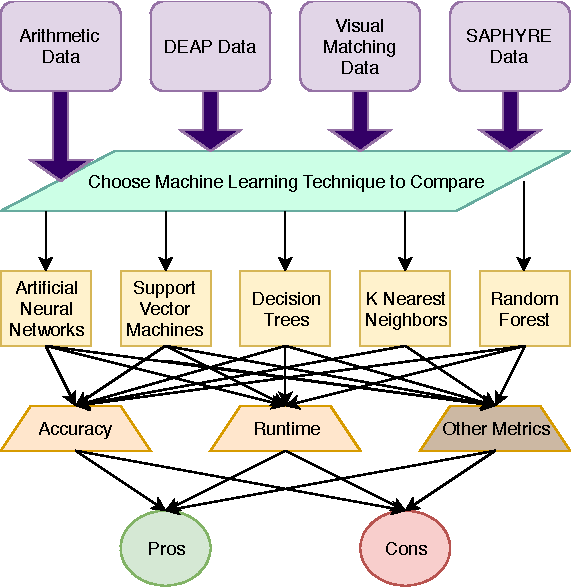
\includegraphics[width=5in]{exp-fig}
\caption{Flowchart of experimental process.}
\label{exp-fig}
\end{figure}

A generalized flowchart of the analysis of alternatives process is presented in Fig.~\ref{exp-fig}. The initial step is to select the dataset to be tested. A description of the datasets used is provided in the next section. Next is to select a machine learning technique to be evaluated. In doing so, three method-specific parameters are compared: two of which are numerical and iterative, and the third of which is more subjective and typically consists of two options. The following step is to evaluate the method based on fundamental metrics such as accuracy and computational runtime. Other metrics for consideration include F1 score, precision, and recall. In viewing and analyzing the results of these metrics, the final step is to determine the pros and cons of the given machine learning method.

%\begin{algorithm}
\begin{figure}
\begin{algorithmic}[1]
\FORALL{datasets}
	\STATE train\_in, val\_in, train\_out, val\_out $\leftarrow$ all possible input and output data	
	\FORALL{methods}
		\FORALL{subjective parameters}
			\FORALL{trials}
				\FOR{first iterative parameter}
					\FOR{second iterative parameter}
						\STATE create classifier using selected method and parameters
						\STATE train classifier
						\STATE results $\leftarrow$ [train. error, val. error, precision, recall, F1, runtime]
						\FORALL{results}
							\STATE result $\leftarrow$ result / no\_iterations
						\ENDFOR
					\ENDFOR
				\ENDFOR
				\FORALL{results}
					\STATE save numerical result values for all iterative parameter combinations
					\STATE save surface plot of values for all iterative parameter combinations
				\ENDFOR
			\ENDFOR
		\ENDFOR
	\ENDFOR
\ENDFOR
\label{full-alg-dagsi1}
\end{algorithmic}
\caption{Pseudocode of complete experimental process.} 
\label{full-alg-dagsi1}
%\end{algorithm}	
\end{figure}

From there, a more comprehensive approach is one that is iterative, traversing each dataset, method, and method-specific parameter. This approach is detailed in Fig.~\ref{full-alg-dagsi1}. Due to the extensive use of \textit{for} loops, the entire process is automatic, inputting the formatted input and output files of each dataset in comma separated value (CSV) format and outputting the results in both numerical and graphical formats. The former consists of a CSV file for each combination of dataset, method, subjective parameter (e.g.~ANN training technique, SVM kernel), and type of evaluation metric. In each file is the numerical result for the selected metric for each iterative parameter combination. The latter format consists of a PDF file containing a three-dimensional surface plot, again for each combination of dataset, method, subjective parameter, and type of evaluation metric. The details of these graphical results are described in Section \ref{dagsi-results}.

The overall process is written in Python and incorporates the scikit-learn package \cite{pedregosa} for access to built-in machine learning functions. The experiment was performed using the Anaconda Python environment on a Windows 10 desktop with an Intel Core i5-3570 3.40 GHz quad core CPU and 16 GB of RAM. In addition, the results were presented as the averages of 10 independent trials for redundancy and consistency.

\subsection{Data Acquisition}

\begin{table}[!t]
\caption{Summary of cognitive workload datasets used in this experiment.}
\renewcommand{\arraystretch}{1.3}
\centering
\resizebox{\textwidth}{!}
{\begin{tabular}{*{4}{l}}
\toprule
Name & Description & Relevance & Source \\ \midrule
Arithmetic & Fear conditioning and cognitive load & EDA resultant from cognitive tasks & co-author of \cite{natarajan} \\
DEAP & Human affective states & EEG recorded from watching video clips & \cite{deap} \\
Visual Matching & Genetic predisposition to alcoholism
 & EEG recorded from observing two images & \cite{uci} \\
SAPHYRE & Pilot skill level & Pilot workload based on heart rate & co-authors of \cite{nittala} \\ \bottomrule
\end{tabular}}

\label{data1}
\end{table}

Table \ref{data1} provides an overview of the four datasets obtained for this research. The second and third sets were obtained from the public domain, while the first and fourth were from a collaborator described in Acknowledgements. Each dataset involves a classification problem of some set of cognitive activities. For instance, adding two repeatedly or subtracting seven repeatedly requires increasingly high amounts of mental load, and thus the goal here is to determine which activity took place at a given time step given the physiological data values at that time and accurately classify which activity (including which specific iteration of add two or subtract seven) took place. By doing so and by interpreting the amount of cognitive load anticipated in each activity, meaningful workload assessment can take place.

\subsubsection{Arithmetic Dataset}

\begin{figure}[!t]
\centering
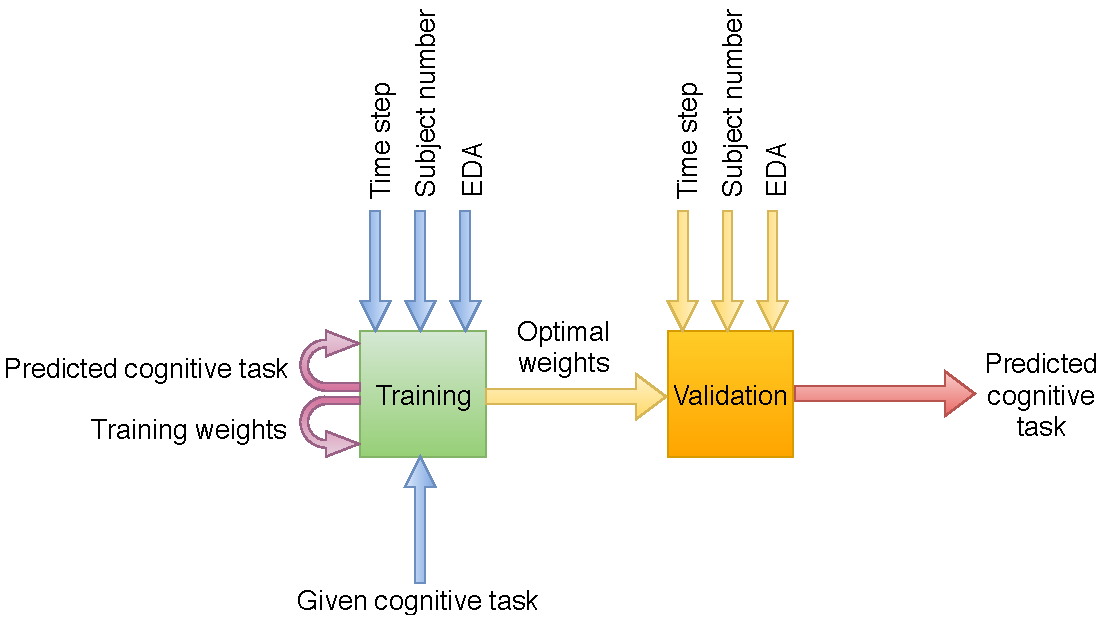
\includegraphics[width=5in]{nata-io}
\caption{Supervised machine learning process for arithmetic data.}
\label{nata-io}
\end{figure}

The first dataset utilized in this research is based on an experiment by [14] in 2016. Natarajan et al.~collected the data for the purposes of evaluating fear conditioning and cognitive load. In turn, the data has been formatted so that it focuses entirely on the latter. To address cognitive workload, the data measures electrodermal activity (EDA) during a series of tests in which a human subject is required to either add 2, subject 7, or rest for 30-second periods. These mental tasks were chosen for the specific purpose of assessing cognitive workload, based on an individual's ability to remember a number and repeatedly, as well as interchangeably, add to or subtract from it. For this research, the data was repurposed so that an ANN or SVM could be modeled to answer one of many possible questions: 

\begin{enumerate}
	\item Given a task number and a time step, what will be a subject's EDA? 
	\item Given a subject's EDA and a time step, which task was he/she performing?
	\item \textit{Given a subject number, his/her EDA, and a time step, what task was he/she performing?}
\end{enumerate} 

The data in this research is formatted to focus on addressing the third and italicized question. The three inputs are self-explanatory as given in the third question, while the sole output is the activity number, which represents the task being performed. Although there are only three unique activities, each nonconsecutive instance of a recurring non-resting task is its own separate activity number for a total of five possible classifications. Figure \ref{nata-io} presents the overall machine learning process for this data.

\subsubsection{DEAP Emotion Recognition Dataset}

\begin{figure}[!t]
\centering
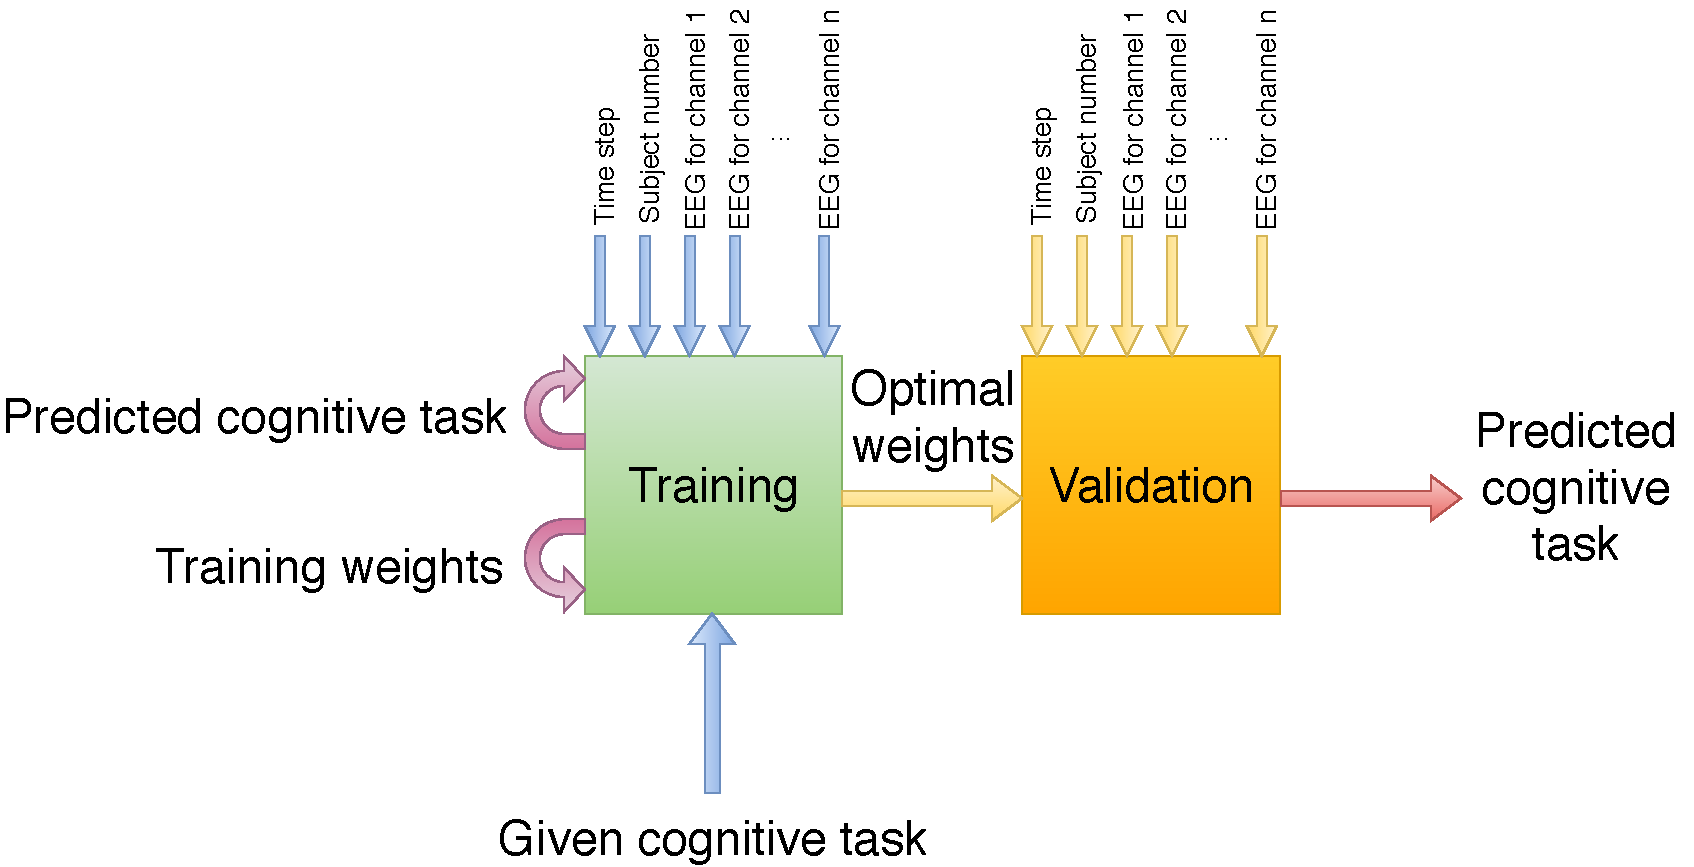
\includegraphics[width=6in]{deap-io}
\caption{Supervised machine learning process for DEAP data.}
\label{deap-io}
\end{figure}

The second dataset named Database for Emotion Analysis using Physiological Signals (DEAP) was obtained from \cite{deap} and examines emotional response to different music videos. Given the sheer amount of visual creativity involved in many music videos, it can be established that the amount of cognitive load required to absorb such videos can vary rapidly. The inputs consist of EEG in 40 channels as well as time step and subject number, while the output is simply the video being watched on the condition that each video has a varying level of cognitive load required to adequately absorb what is being watched. Therefore, this data can be modeled based on the question: \textit{Given a time step, a subject number, and the subject’s EEG, what task was he or she performing?} Fig. \ref{deap-io} provides an overview of this dataset's machine learning process as well as its inputs and outputs.

\subsubsection{EEG Visual Matching Dataset}

\begin{figure}[!t]
\centering
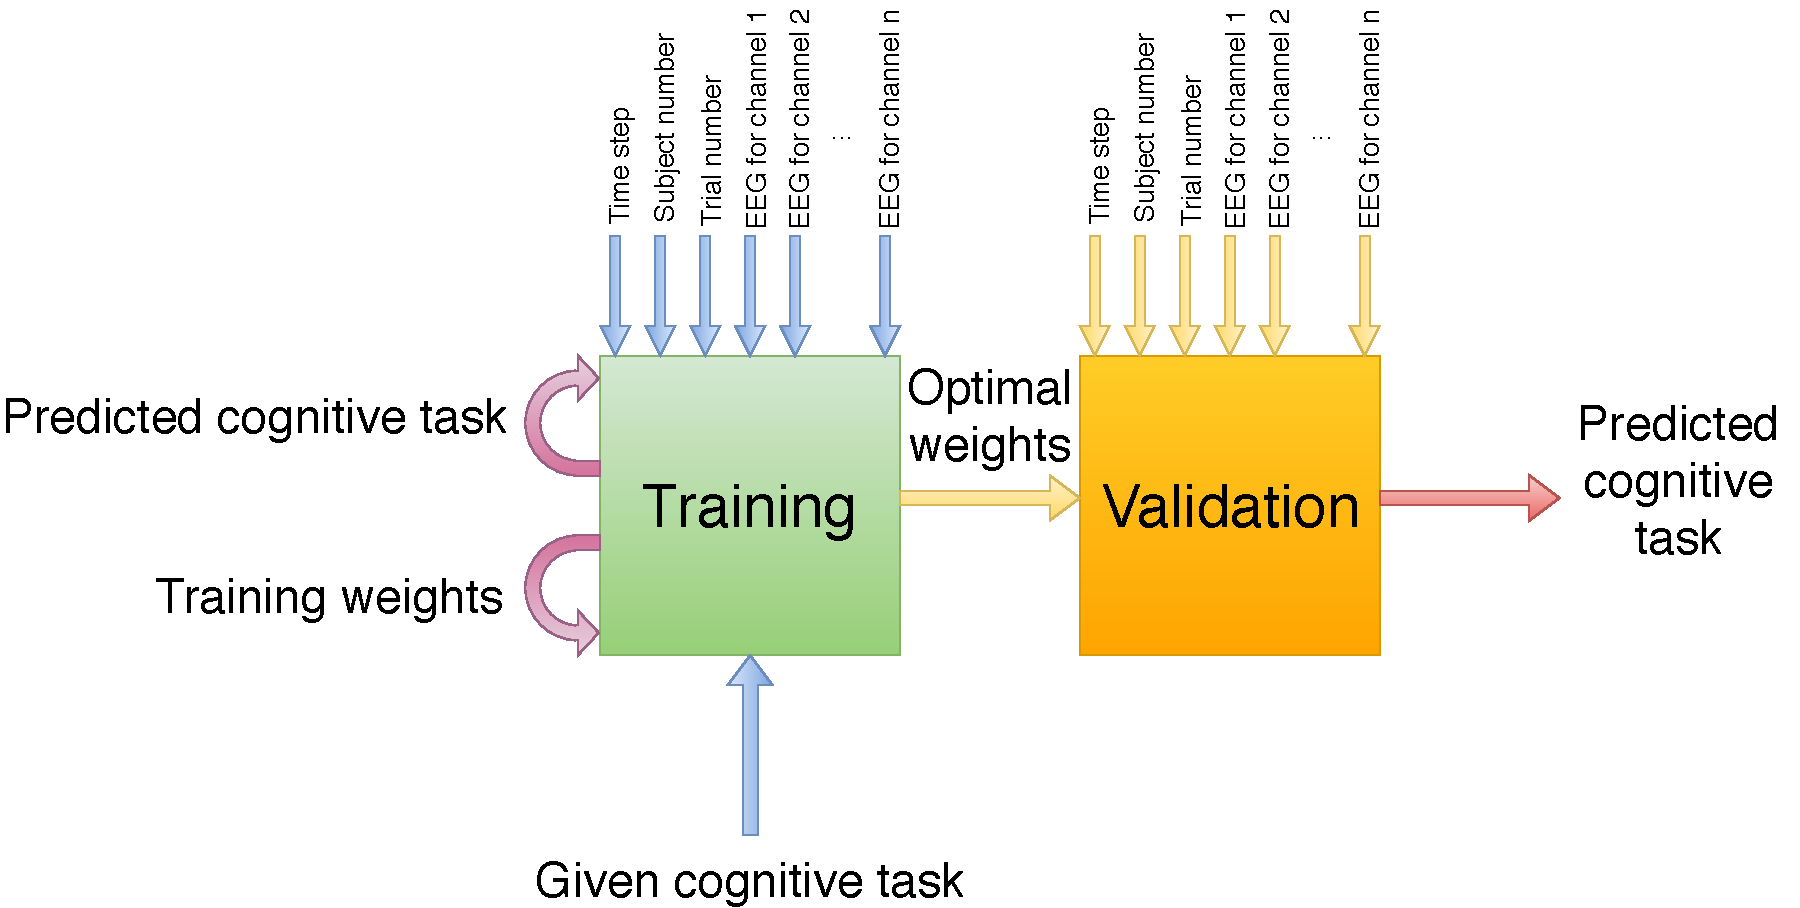
\includegraphics[width=6in]{vismatch-io}
\caption{Supervised machine learning process for visual matching data.}
\label{vismatch-io}
\end{figure}

This third dataset was obtained from \cite{uci}, which examines genetic predisposition among alcoholic and control subjects based on EEG correlation. Over the course of 122 subjects and 120 trials, the cognitive activity consisted of being shown either a single image, two matching images, or two non-matching images. Each of these three activities was considered as separate classifications between alcoholic subjects and control subjects, hence a total of six possible output choices. Thus, this classification problem is modeled from the modified question: \textit{Given a time step, a subject number, a trial number, and the subject’s EEG across 64 channels, what task was he or she performing?} Fig. \ref{vismatch-io} depicts an overview of this data's machine learning process as well as the inputs and outputs.

\subsubsection{SAPHYRE Pilot Dataset}
%
%\begin{figure}[!t]
%\centering
%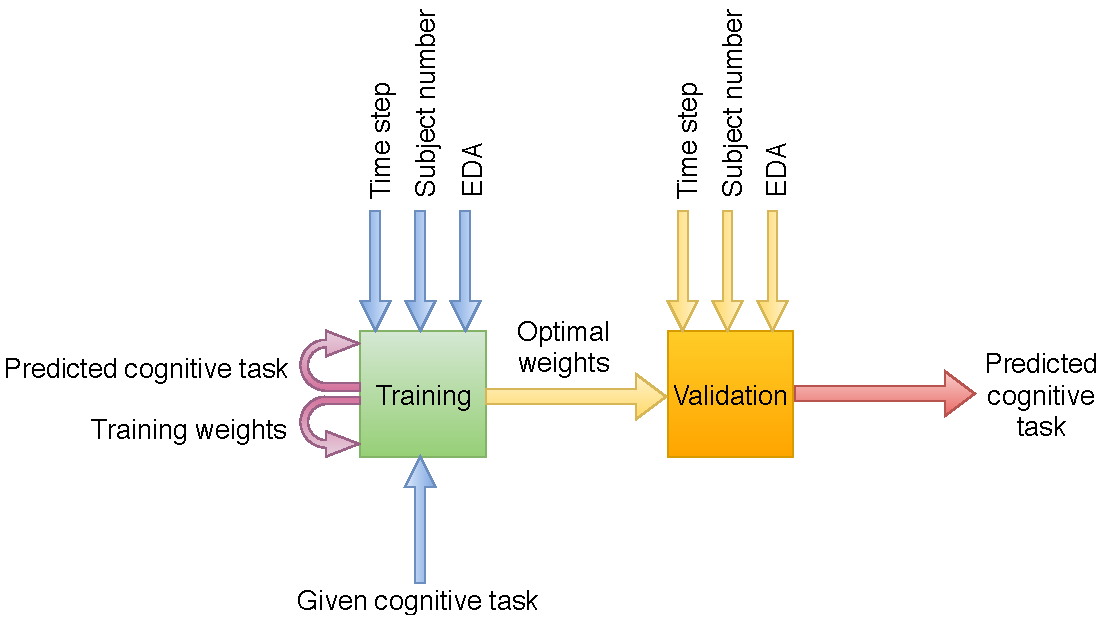
\includegraphics[width=6in]{nata-io}
%\caption{Supervised machine learning process for SAPHYRE data.}
%\label{saphyre-io}
%\end{figure}

The final dataset bears the most relevance to the subject of flight safety, as the human subjects are actual pilots. In addition, this data consists of both physiological inputs and navigational/operational inputs. Due to the large amount of unique inputs, there is no flowchart provided here. Instead the inputs are listed as follows:
\begin{enumerate}
\item Time step
\item Subject number
\item Heart rate
\item Aileron
\item Elevator
\item Rudder
\item Throttle
\item Heading
\item Altitude
\item Latitude
\item Longitude
\item Speed
\item Proposed latitude
\item Proposed longitude
\item Distance from path
\end{enumerate}
From there, the output classification is a combination of flight route, flight path, and pilot skill level, which is given by
\begin{equation}
C = 5sp+r,
\end{equation}
where $C$ is the output classification, $s$ denotes a pilot's skill level (1 for expert, 0 for novice), $p$ is the path number, and $r$ represents the route number. This is on the basis that cognitive workload levels could vary with skill level. In other words, a more experienced pilot may need less mental load to complete the same task undertaken by a novice pilot. This is also based on the fact that the complexity of different routes or paths could also contain varying levels of cognitive load.
Thus, the overall problem given by this data models the question: \textit{Given the above inputs, what are the route, path, and pilot skill level?}

\subsection{Evaluation Metrics}

To ensure a thorough and meaningful analysis of the experimental results, five different metrics were selected for evaluating the machine learning techniques, with the majority of importance lying within accuracy and runtime.

In scikit-learn, accuracy is determined by the score function, which in each classifier is the mean accuracy. Mean accuracy is simply the ratio of correct predictions to total possible predictions. This is considered to be a tough evaluation metric, as a classification is only considered correct if there is an exact match between the predicted output and the actual output, as opposed to accuracy in a regression problem, in which evaluation is based on the closeness between a prediction and an output. Because each of the candidate machine learning methods are all supervised learning techniques, accuracy in this experiment is divided into training accuracy and validation accuracy, in which the training samples and validation samples are respectively evaluated individually.

Computational runtime is the amount of time required to complete the training and evaluation phases for each combination of dataset, method, and other parameters. Runtime is dependent on both efficiency of the ML method and the computing resources available. Thus, every facet of this experiment is done on the same hardware and software, the specifications of which are discussed at the beginning of Section \ref{dagsi-mm}.

Other relevant evaluation metrics include precision, which differs from accuracy in that it is the ability of a classifier to not predict a positive output for a sample with a negative one \cite{pedregosa}. It is defined as the ratio of number of true positives to the sum of both true and false positives. Recall, however, is the ability to find all the positive samples and is calculated as the ratio of true positives to the true positives and false negatives. Meanwhile, the F1 score is a weighted average of precision and recall, defined by
\begin{equation}
F1 = 2 * \frac{precision * recall}{precision + recall}.
\end{equation}
With exception of runtime, all of the evaluation scores are normalized values, in which 1 is a perfect score and 0 is the lowest possible.

\section{Experimental Results}
\label{dagsi-results}

Extensive results of the entire experimental procedure are given in the following subsections, figures, and tables. For organizational purposes, each subsection corresponds to each of the four datasets. Within each subsection are two tables that summarizes the results for each combination of technique and subjective parameter (e.g.~ANN optimizer, SVM kernel). The result types consist of training accuracy, validation accuracy, and runtime (in seconds) in the first table as well as precision, recall, and F1 scores in the second table, with each category consisting of a minimum value, a maximum value, and a mean value. 

Each subsection also consists of five figures, one for each ML method, with each figure divided into 3-by-2 subfigures. Each column corresponds to the subjective parameter of the method (such as gini and entropy criteria for DT and RF), while each row corresponds to the type of evaluation metric presented. In this case, the focus is only only three types: validation accuracy, F1 score, and runtime. Each subfigure is a three-dimensional surface plot with x and y axes corresponding to the numerical, or iterative experimental parameters, while the z axis is the evaluation result.

\subsection{Arithmetic Dataset}

\begin{table}[!t]
\caption{Summary of training accuracy, validation accuracy, and computational runtime on arithmetic data.}
\renewcommand{\arraystretch}{1.3}
\centering
%\resizebox{\textwidth}{!}
{\begin{tabular}{*{10}{l}}
\toprule
& \multicolumn{3}{l}{Train. Accuracy} & \multicolumn{3}{l}{Val. Accuracy} & \multicolumn{3}{l}{Runtime (s)} \\
Technique & Max & Min & Mean & Max & Min & Mean & Max & Min & Mean \\ \midrule
ANN SGD & .990 & .405 & .707 & .990 & .403 & .706 & 24.8 & .995 & 8.68 \\
ANN L-BFGS & .999 & .399 & .704 & .998 & .393 & .703 & 43.1 & .229 & 10.8 \\
KNN Uniform & 1.00 & .988 & .994 & .991 & .980 & .985 & .473 & .287 & .348 \\
KNN Distance & 1.00 & 1.00 & 1.00 & .991 & .987 & .989 & .482 & .297 & .353 \\
SVM Linear & .437 & .435 & .436 & .442 & .431 & .436 & 7.73 & 6.63 & 7.21 \\
SVM RBF & .993 & .892 & .983 & .987 & .891 & .977 & 10.1 & 2.70 & 4.38 \\
DT Gini & 1.00 & .999 & .999 & .999 & .998 & .999 & .225 & .203 & .210 \\
DT Entropy & 1.00 & .999 & .999 & .999 & .998 & .999 & .230 & .205 & .216 \\
RF Gini & 1.00 & .998 & .999 & .998 & .997 & .998 & .331 & .310 & .318 \\
RF Entropy & 1.00 & .998 & .999 & .998 & .996 & .997 & .405 & .356 & .368 \\ \bottomrule
\end{tabular}}

\label{tvr-nata}
\end{table}

Table \ref{tvr-nata} provides an overview of the accuracy and runtime results for the arithmetic dataset. In terms of accuracy alone, nine out of ten technique combinations show highly promising results for this dataset, as each one other than SVM with the linear kernel provides up to at least 99\% accuracy for both training and validation. In addition, DT, RF, and KNN provide perfect scores in training accuracy in some scenarios. In the case of the latter, every combination of iterative parameters results in 100\% accuracy. In terms of ranges of values, some methods are better at producing high accuracy across the board than others. In the case of DT and RF, the lowest accuracy value produced is still over 99\%, with the former having a slight edge in minimum and average accuracy values. ANN, meanwhile, produces the widest range of accuracy values, ranging anywhere from 39.9\% to 99.8\%. This is particularly true for the L-BFGS optimizer, as both the upper and lower limits are produced by this parameter. In terms of computational runtime, DT continues to maintain supremacy in this dataset, with maximum runtime values that rival even the minimum values from other methods. ANN and SVM appear to do the worst in terms of runtime and efficiency, as all their runtime values are the only ones to exceed half a second, often by an overwhelming margin. SVM has the most consistently high runtime, as every value exceeds one second, while ANN has the greatest maximum value as well as the widest range of values, spanning roughly from a quarter of a second to three quarters of a minute. Overall, it can be declared so far that decision trees are the most optimal method for the arithmetic dataset from all positive angles.

\begin{table}[!t]
\caption{Summary of F1, precision, and recall scores on arithmetic data.}
\renewcommand{\arraystretch}{1.3}
\centering
%\resizebox{\textwidth}{!}
{\begin{tabular}{*{10}{l}}
\toprule
& \multicolumn{3}{l}{F1} & \multicolumn{3}{l}{Precision} & \multicolumn{3}{l}{Recall} \\
Technique & Max & Min & Mean & Max & Min & Mean & Max & Min & Mean \\ \midrule
ANN SGD & .990 & .121 & .567 & .992 & .087 & .555 & .992 & .200 & .609 \\
ANN L-BFGS & .998 & .121 & .570 & .998 & .086 & .557 & .998 & .200 & .612 \\
KNN Uniform & .991 & .981 & .986 & .994 & .984 & .989 & .991 & .976 & .984 \\
KNN Distance & .992 & .988 & .990 & .992 & .987 & .990 & .991 & .987 & .990 \\
SVM Linear & .120 & .123 & .121 & .088 & .086 & .087 & .200 & .200 & .200 \\
SVM RBF & .988 & .901 & .979 & .987 & .871 & .973 & .990 & .950 & .986 \\
DT Gini & .999 & .998 & .999 & .999 & .998 & .999 & .999 & .998 & .999 \\
DT Entropy & .999 & .998 & .999 & .999 & .998 & .999 & .999 & .998 & .999 \\
RF Gini & .998 & .997 & .998 & .999 & .997 & .998 & .998 & .997 & .998 \\
RF Entropy & .998 & .996 & .997 & .998 & .996 & .997 & .998 & .997 & .998 \\ \bottomrule
\end{tabular}}

\label{fpr-nata}
\end{table}

Table \ref{fpr-nata} is an overview for the remaining three metrics: the precision, recall, and F1 scores. From here, DT is still the most highly scored method, as each set of metric values ranges from .998 to .999. RF comes in at a close second with only slightly lower values. ANN again produces the widest range of values in all three cases, while SVM's linear kernel continues to produce consistently poor results. Thus, DT is still the most superior method for this dataset. In terms of non-runtime metrics, both gini and entropy criteria produce the same ranges of scores. Thus, the only remaining way to compare the two is with runtime, in which case gini produces slightly faster speed and efficiency, thereby making DT with gini the best method for this dataset.

\begin{figure*}\centering
\subfloat[Validation error for L-BFGS optimizer\label{nata-ann-val-lbfgs}]
		{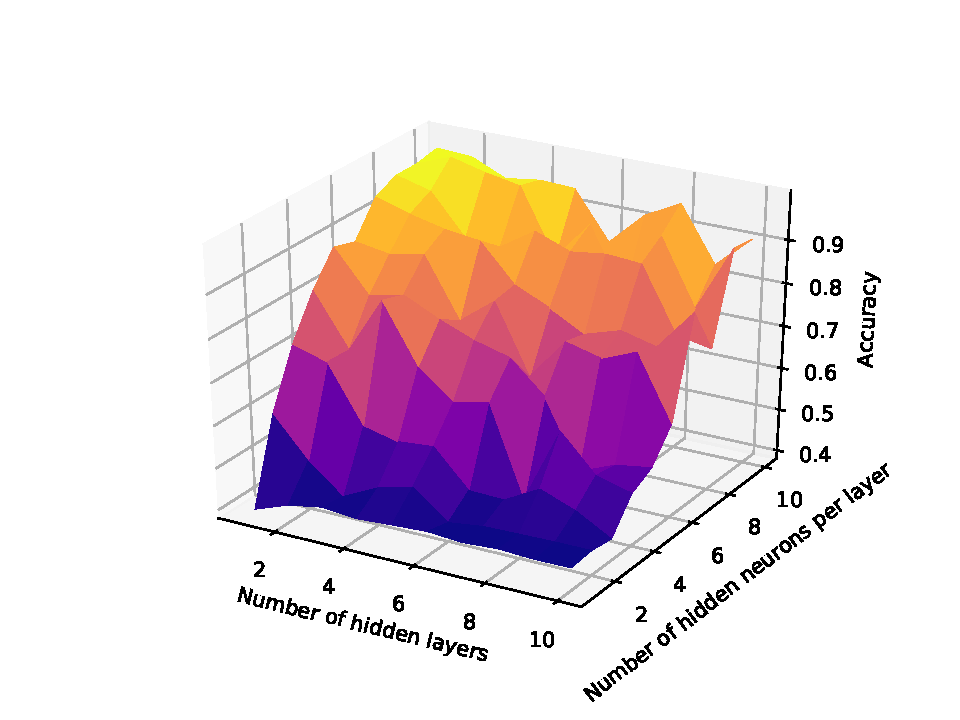
\includegraphics[width=0.5\textwidth]{nata/nata/ANN/lbfgs_val}}
	\hfill	
\subfloat[Validation error for SGD optimizer\label{nata-ann-val-sgd}]
		{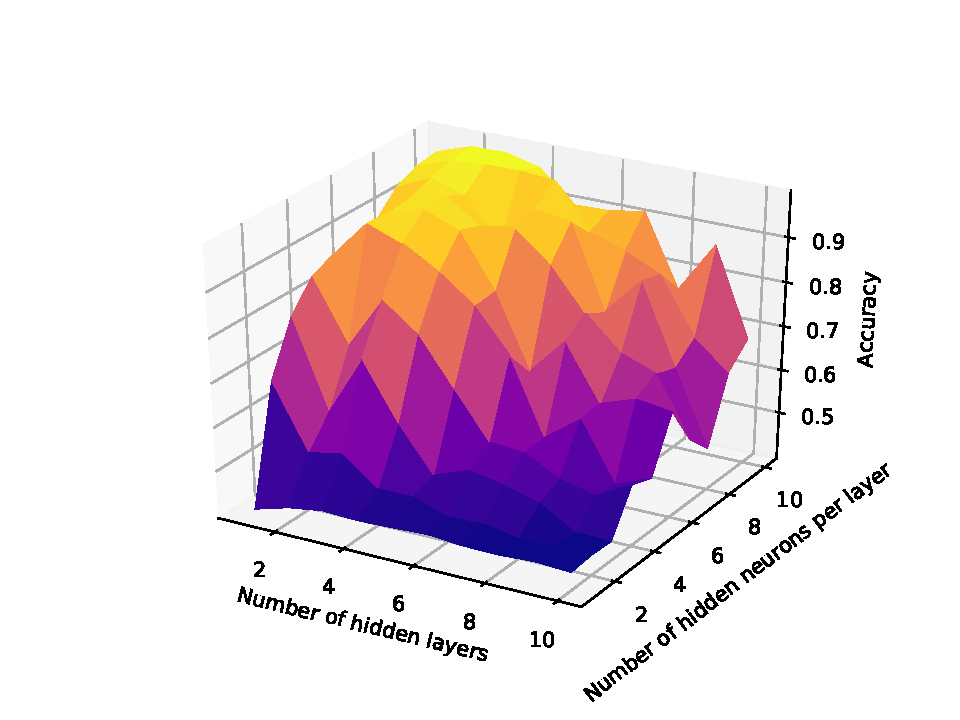
\includegraphics[width=0.5\textwidth]{nata/nata/ANN/sgd_val}}
		
\subfloat[F1 score for L-BFGS optimizer\label{nata-ann-f1-lbfgs}]
		{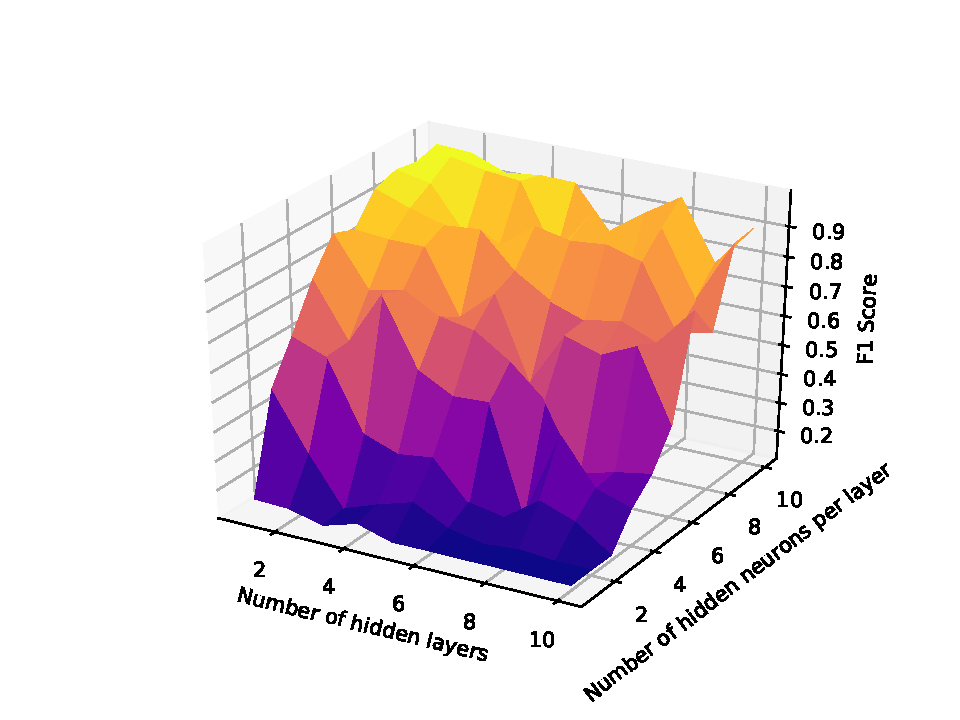
\includegraphics[width=0.5\textwidth]{nata/nata/ANN/lbfgs_f1}}
	\hfill	
\subfloat[F1 score for SGD optimizer\label{nata-ann-f1-sgd}]
		{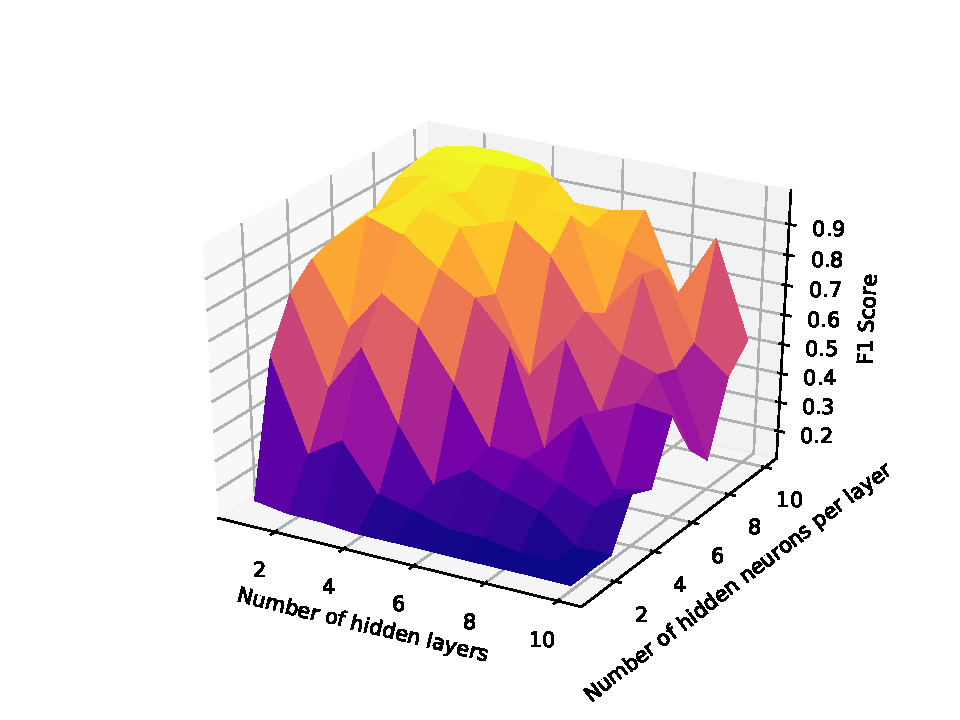
\includegraphics[width=0.5\textwidth]{nata/nata/ANN/sgd_f1}}
		
\subfloat[Computational runtime for L-BFGS optimizer\label{nata-ann-runtime-lbfgs}]
		{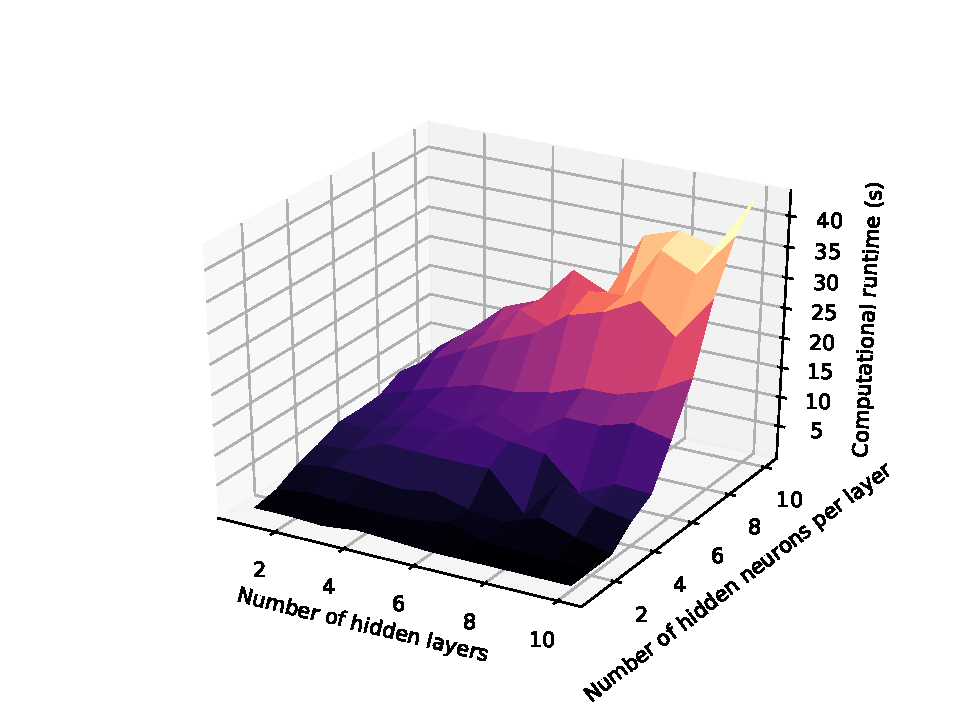
\includegraphics[width=0.5\textwidth]{nata/nata/ANN/lbfgs_runtime}}
	\hfill	
\subfloat[Computational runtime for SGD optimizer\label{nata-ann-runtime-sgd}]
		{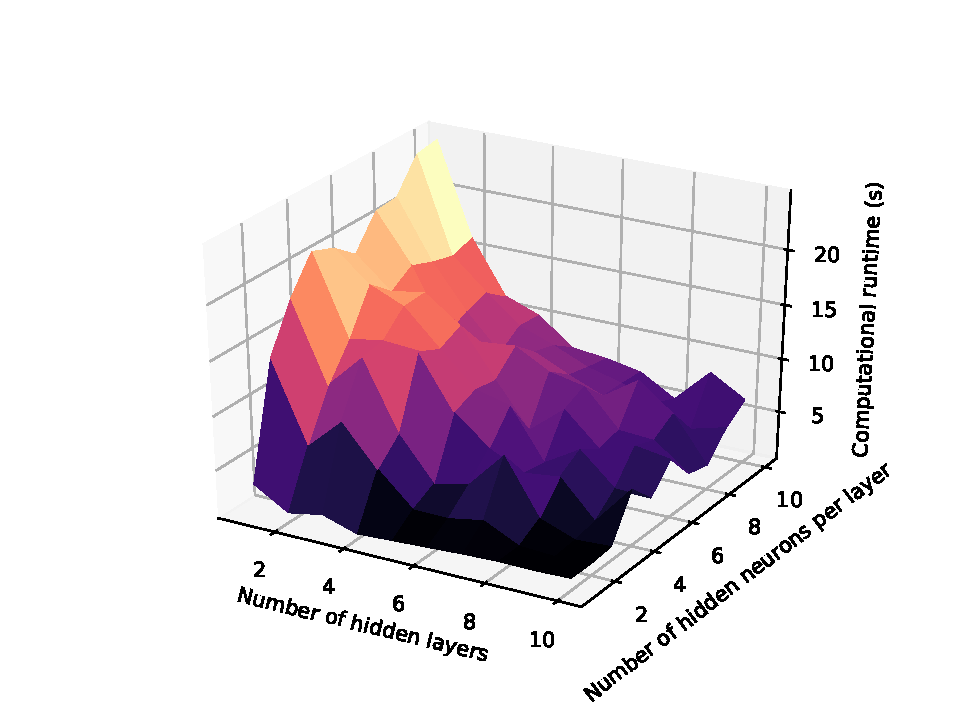
\includegraphics[width=0.5\textwidth]{nata/nata/ANN/sgd_runtime}}
						
\caption{Plots of validation accuracy, F1 score, and computational runtime for ANN on arithmetic data for L-BFGS and SGD optimizers.}
	\label{ann-nata}
	\end{figure*}

Fig.~\ref{ann-nata} provides graphical results for ANN on the Natajan dataset. From here, the patterns and trends in metric variability are more visible. As seen in 
Subfig.~\ref{nata-ann-val-lbfgs}, accuracy increases in proportion to the number of hidden neurons in the neural network. In terms of number of hidden layers, however, there does not seem to be any significant correlation. For 
Subfig.~\ref{nata-ann-val-sgd}, both axes follow noticeable patterns. The number of neurons still maintains a direct correlation with accuracy while an increase in the number of hidden layers actually decreases the accuracy. The plots of F1 scores in 
Subfig.~\ref{nata-ann-f1-lbfgs} and 
\ref{nata-ann-f1-sgd} follow the same trends and share similar values overall. The runtime results in 
Subfigs.~\ref{nata-ann-runtime-lbfgs} and 
~\ref{nata-ann-runtime-sgd} follow uniquely different trends, even from one another. In both cases, an increase in the number of hidden neurons results in a greater runtime. However, in terms of number of hidden layers, runtime actually decreases in SGD in proportion to number of layers increasing, while L-BFGS runtime increases. Both of these trends, meanwhile are at near exponential rates, as seen in the curves respective to the x axis. This is again due to the wide range of runtime values produced by the ANN.

\begin{figure*}\centering
\subfloat[Validation error for linear kernel\label{nata-svm-val-linear}]
		{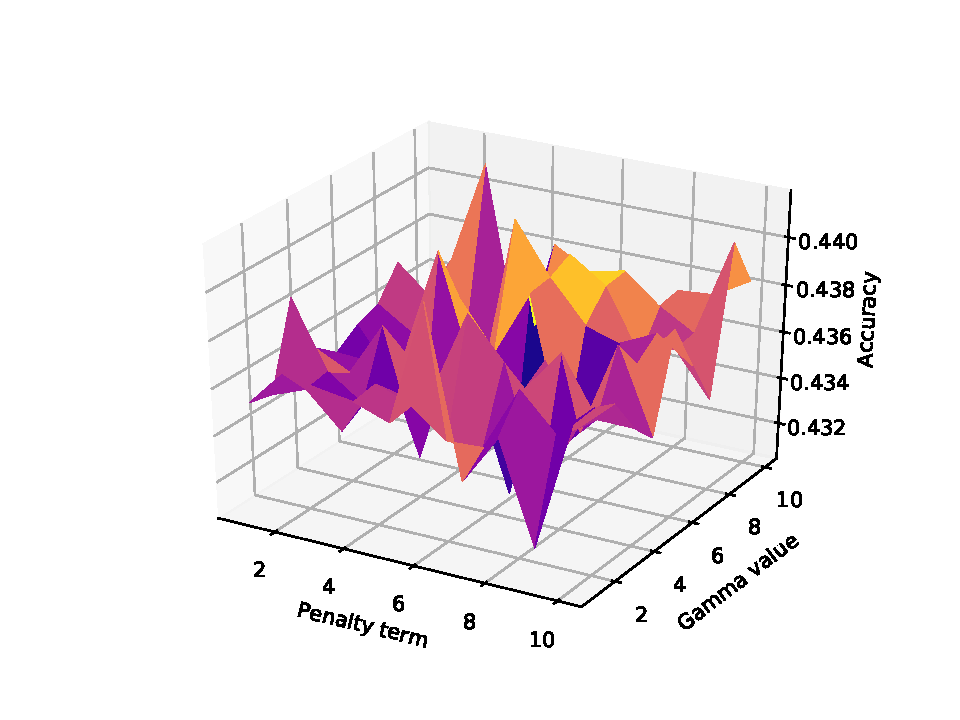
\includegraphics[width=0.5\textwidth]{nata/nata/SVM/linear_val}}
	\hfill	
\subfloat[Validation error for RBF kernel\label{nata-svm-val-rbf}]
		{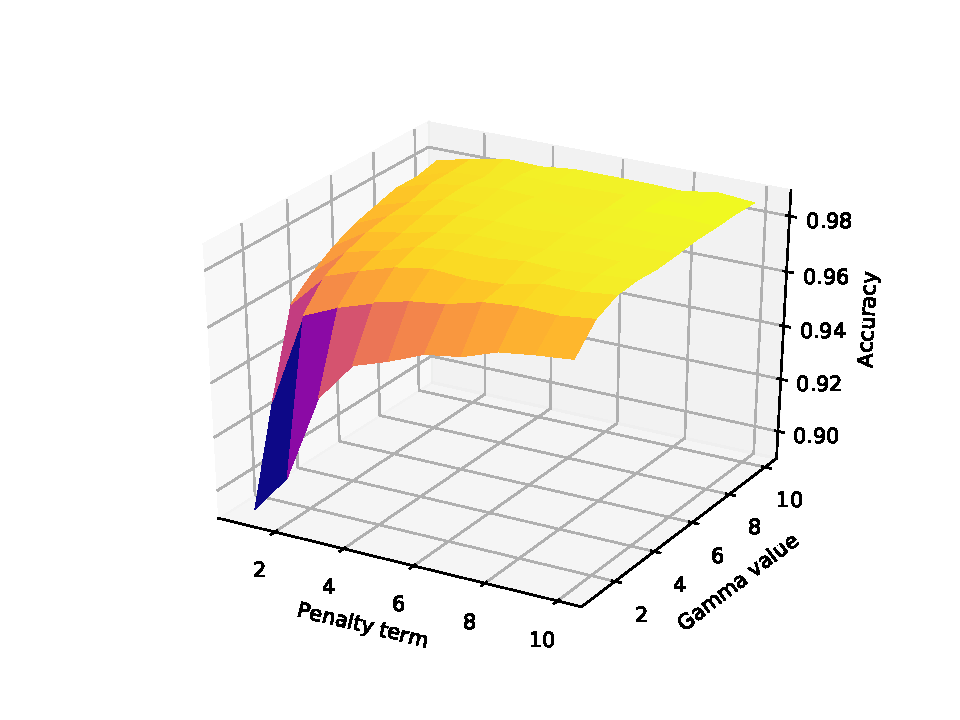
\includegraphics[width=0.5\textwidth]{nata/nata/SVM/rbf_val}}
		
\subfloat[F1 score for linear kernel\label{nata-svm-f1-linear}]
		{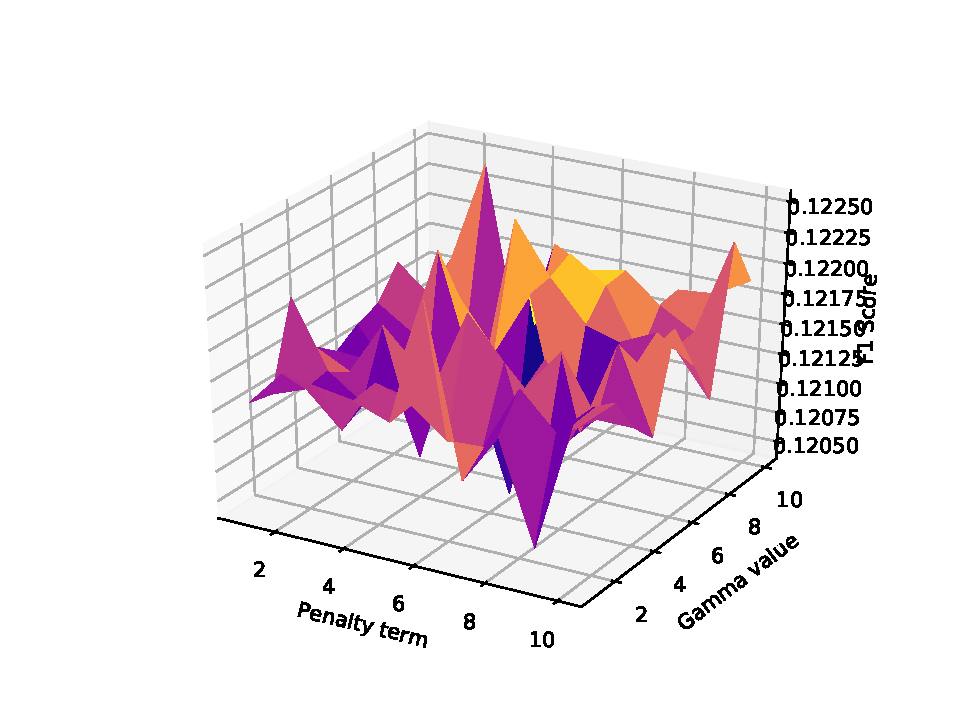
\includegraphics[width=0.5\textwidth]{nata/nata/SVM/linear_f1}}
	\hfill	
\subfloat[F1 score for RBF kernel\label{nata-svm-f1-rbf}]
		{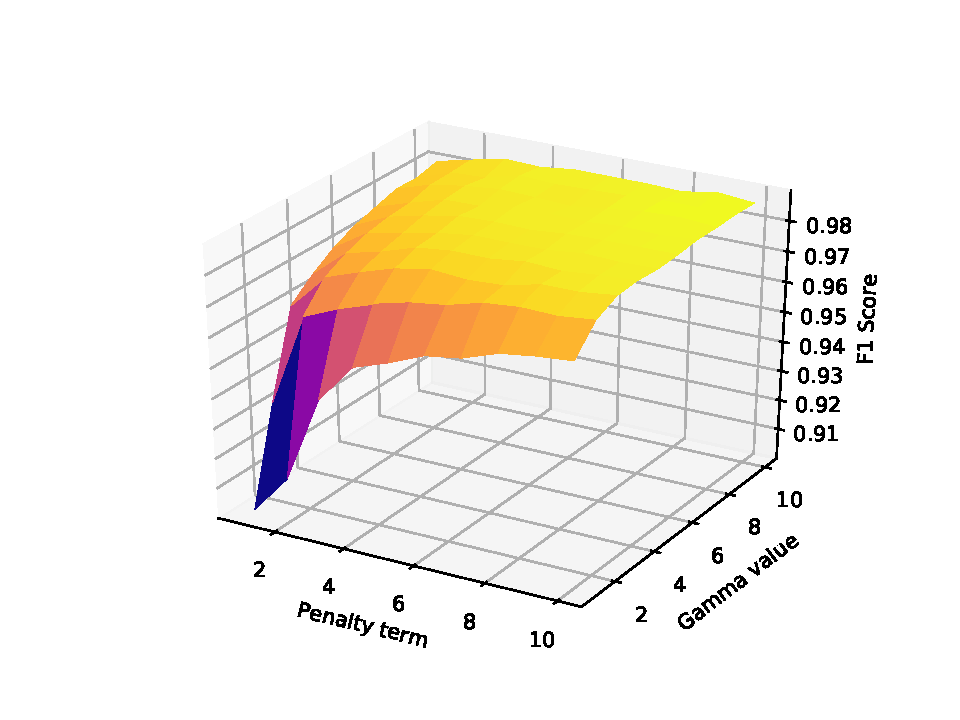
\includegraphics[width=0.5\textwidth]{nata/nata/SVM/rbf_f1}}
		
\subfloat[Computational runtime for linear kernel\label{nata-svm-runtime-linear}]
		{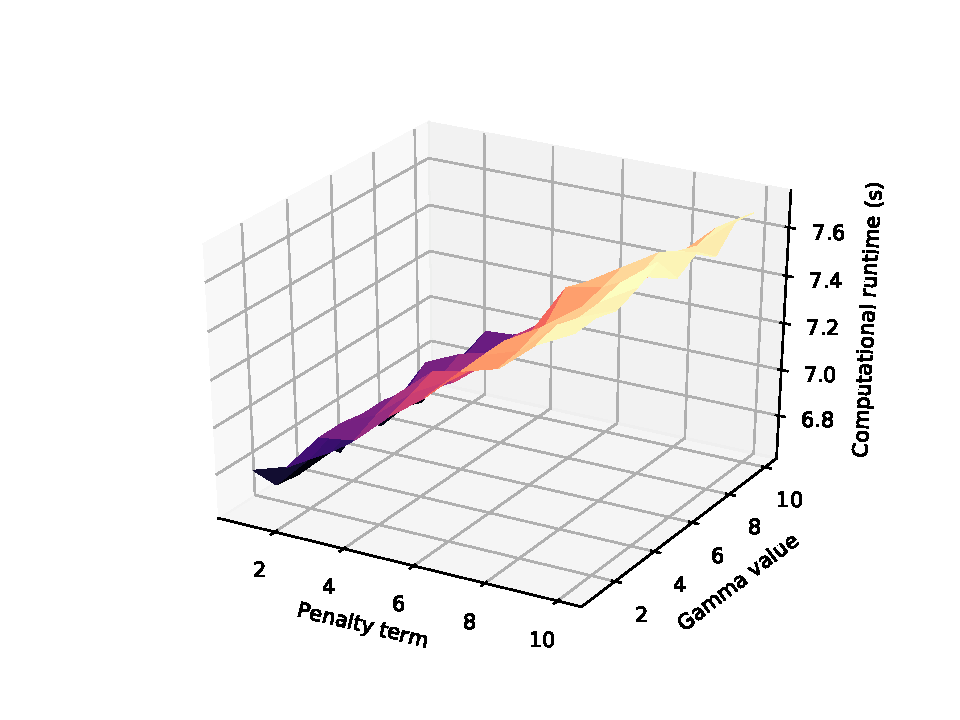
\includegraphics[width=0.5\textwidth]{nata/nata/SVM/linear_runtime}}
	\hfill	
\subfloat[Computational runtime for linear kernel\label{nata-svm-runtime-rbf}]
		{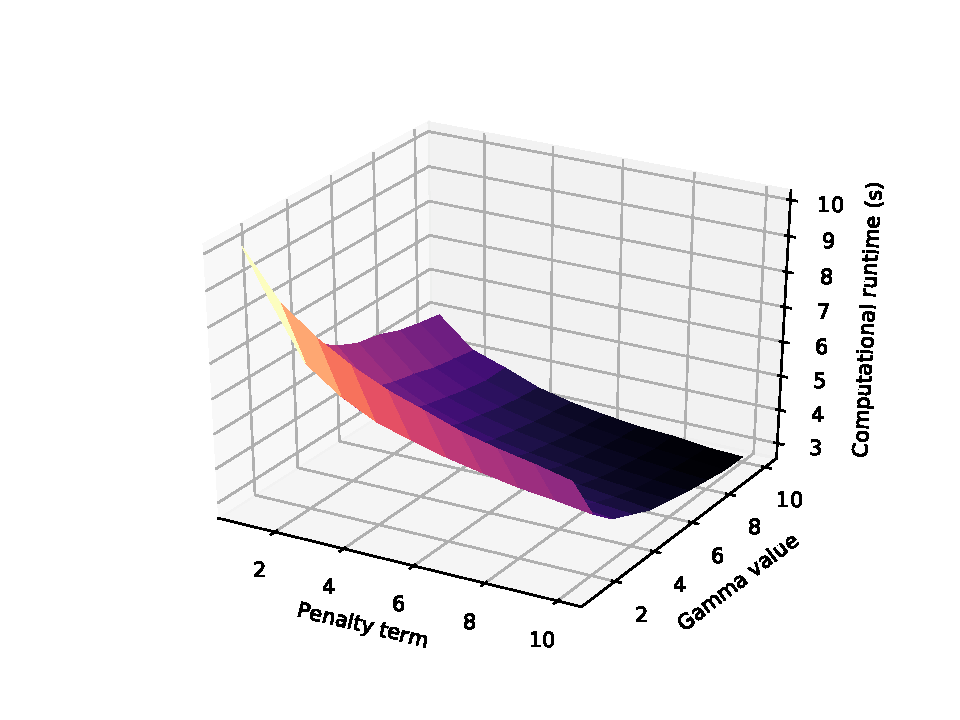
\includegraphics[width=0.5\textwidth]{nata/nata/SVM/rbf_runtime}}
						
\caption{Plots of validation accuracy, F1 score, and computational runtime for SVM on arithmetic data for linear and RBF kernels.}
	\label{svm-nata}
	\end{figure*}
	
When turning to SVM results depicted in Fig.~\ref{svm-nata}, it can be observed that under the linear kernel, there no noticeable correlations relating validation accuracy or F1 score with penalty term or gamma value. This is primarily because the differences in accuracy values are highly minimal (.008 or 0.8\% for accuracy, 0.002 for F1). It is also worth recalling that this is the SVM kernel and only method configuration for this dataset in which accuracy is consistently low (in this case, never exceeding 50\%). F1 score is also extremely low in this case, never exceeding an eighth of a perfect score. RBF accuracy, however, follows more predictable trends with higher values. In both axes, accuracy and F1 increase proportionally to both iterative variables, but primarily at lower values. When both axis values are four or more, the curve becomes relatively flat. As for runtime, both kernels have distinctly different effects on this metric. In the linear kernel, runtime increases with penalty term with no noticeable change with gamma value, while in RBF, the runtime is inversely proportional to either variable.

\begin{figure*}\centering
\subfloat[Validation error for uniform weights\label{nata-knn-val-uniform}]
		{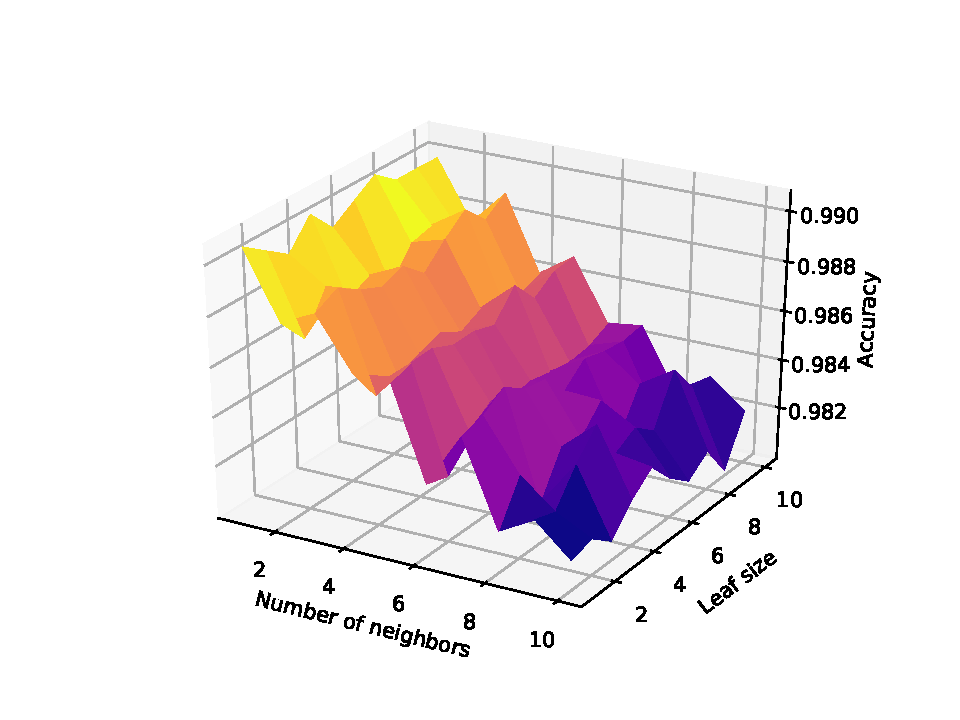
\includegraphics[width=0.5\textwidth]{nata/nata/KNN/uniform_val}}
	\hfill	
\subfloat[Validation error for distance weights\label{nata-knn-val-distance}]
		{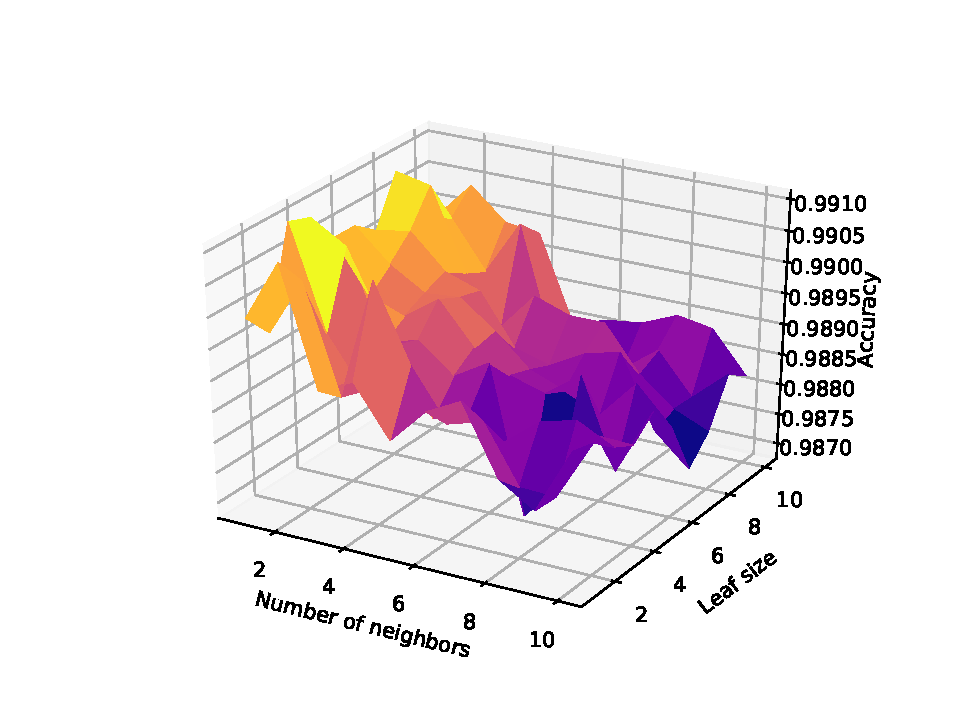
\includegraphics[width=0.5\textwidth]{nata/nata/KNN/distance_val}}
		
\subfloat[F1 score for uniform weights\label{nata-knn-f1-uniform}]
		{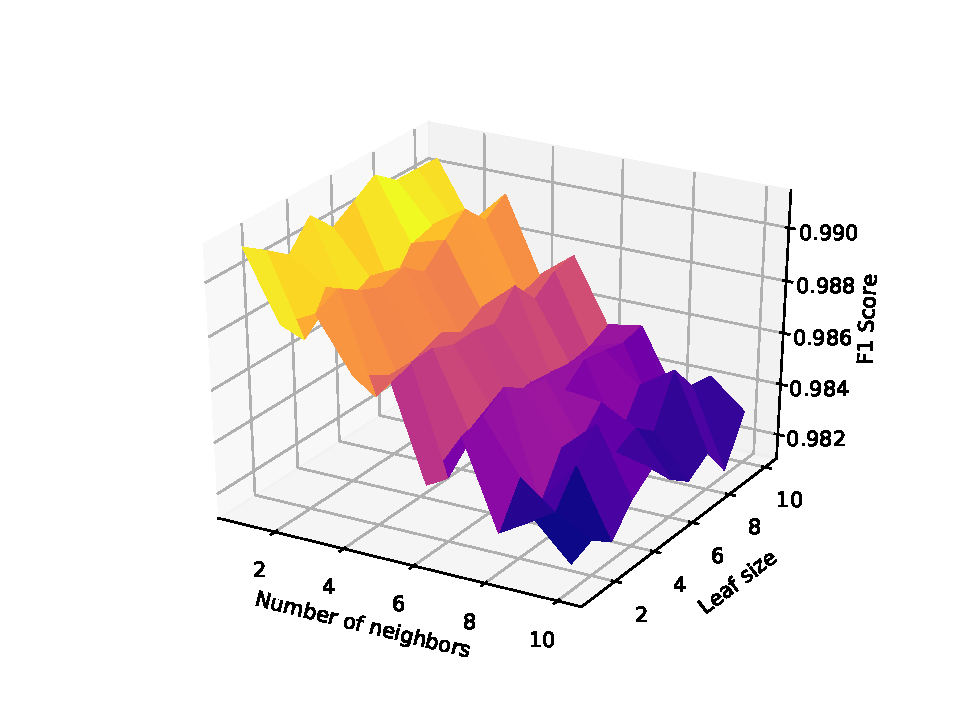
\includegraphics[width=0.5\textwidth]{nata/nata/KNN/uniform_f1}}
	\hfill	
\subfloat[F1 score for distance weights\label{nata-knn-f1-distance}]
		{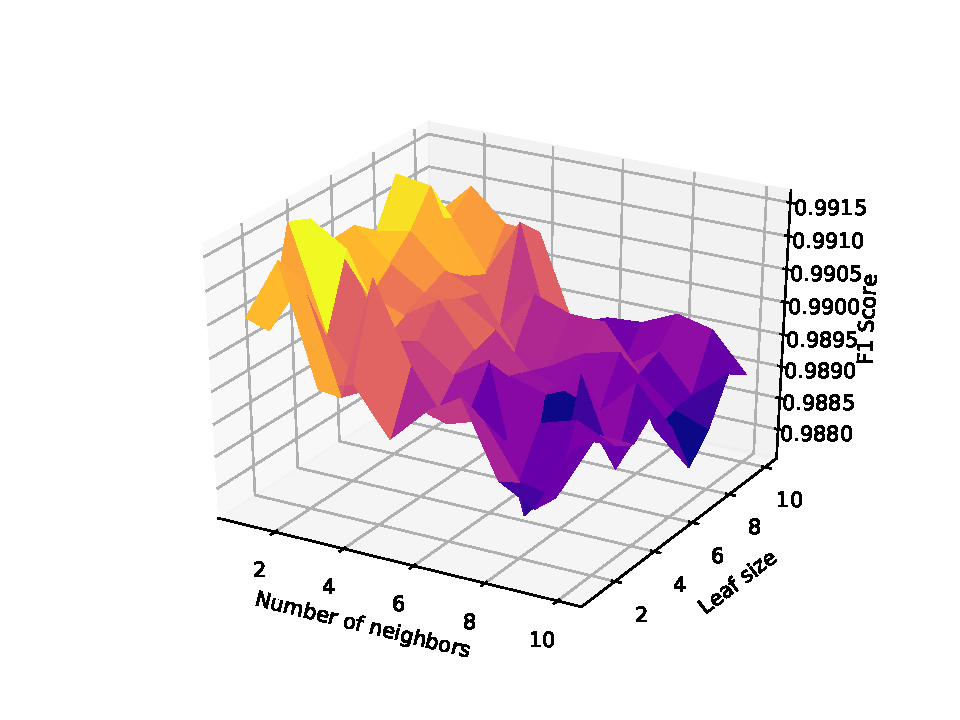
\includegraphics[width=0.5\textwidth]{nata/nata/KNN/distance_f1}}
		
\subfloat[Computational runtime for uniform weights\label{nata-knn-runtime-uniform}]
		{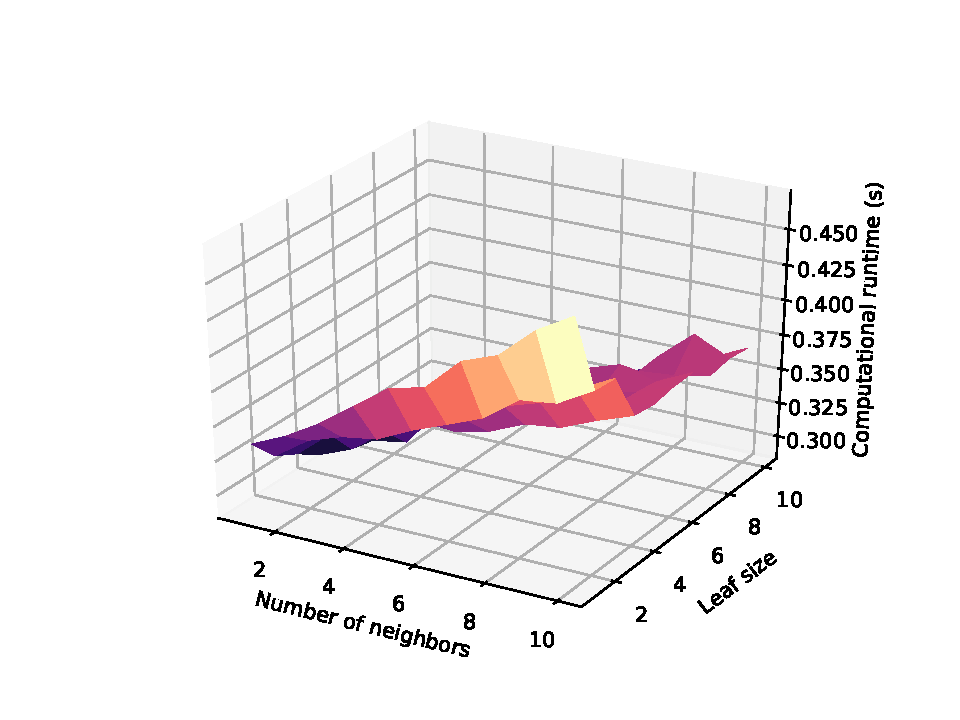
\includegraphics[width=0.5\textwidth]{nata/nata/KNN/uniform_runtime}}
	\hfill	
\subfloat[Computational runtime for distance weights\label{nata-knn-runtime-distance}]
		{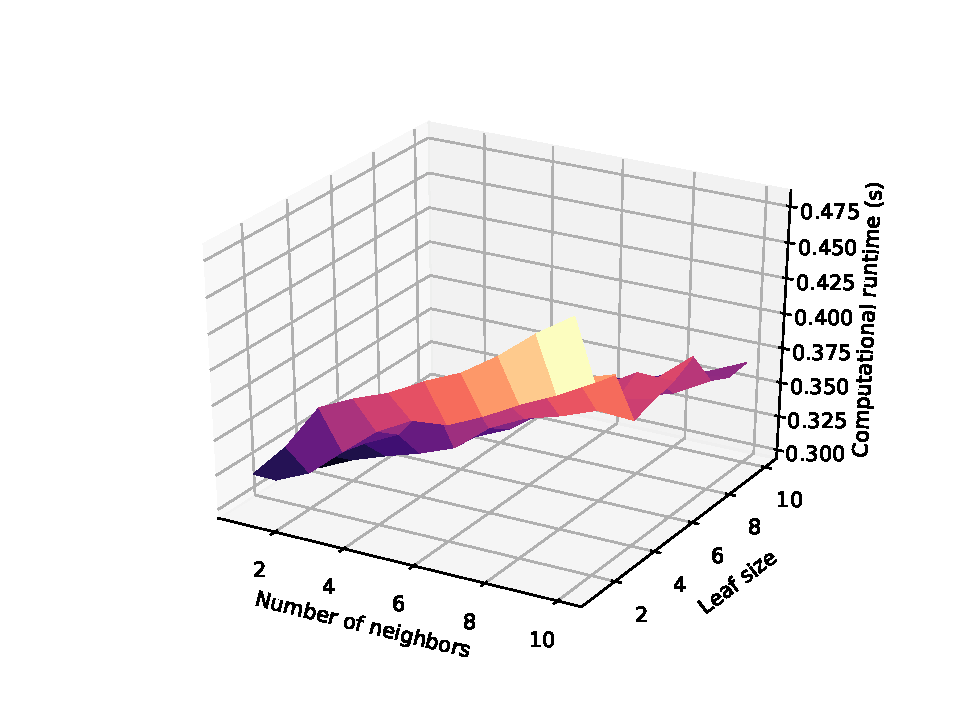
\includegraphics[width=0.5\textwidth]{nata/nata/KNN/distance_runtime}}
						
\caption{Plots of validation accuracy, F1 score, and computational runtime for KNN on arithmetic data for uniform and distance weights.}
	\label{knn-nata}
	\end{figure*}
	
A similar set of graphical results for KNN is presented in Fig.~\ref{knn-nata}. In the case of uniform weights, validation error and F1 score seem to decrease as the number of neighbors increases, while there is no noticeable change as leaf size changes. For distance weights, both axes have an inverse proportionality with accuracy, although it is less noticeable in leaf size.	For runtime, both weight configurations involve increased runtime as the number of neighbors increases and as the leaf size decreases. It is also worth noting that these slopes are much less steep compared to the ANN results, as the ranges of values are much closer together. More specifically, all accuracy and F1 values range from .98 to .99, while all runtime values are within 0.15 seconds of one another. 

\begin{figure*}\centering
\subfloat[Validation error for gini criterion\label{nata-dt-val-gini}]
		{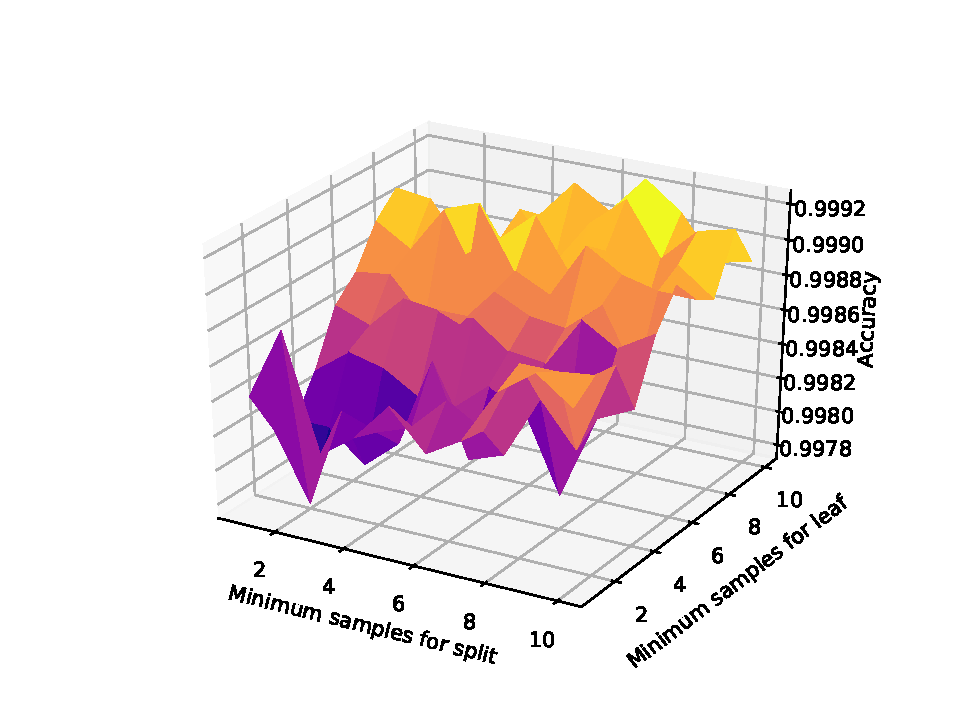
\includegraphics[width=0.5\textwidth]{nata/nata/DT/gini_val}}
	\hfill	
\subfloat[Validation error for entropy criterion\label{nata-dt-val-entropy}]
		{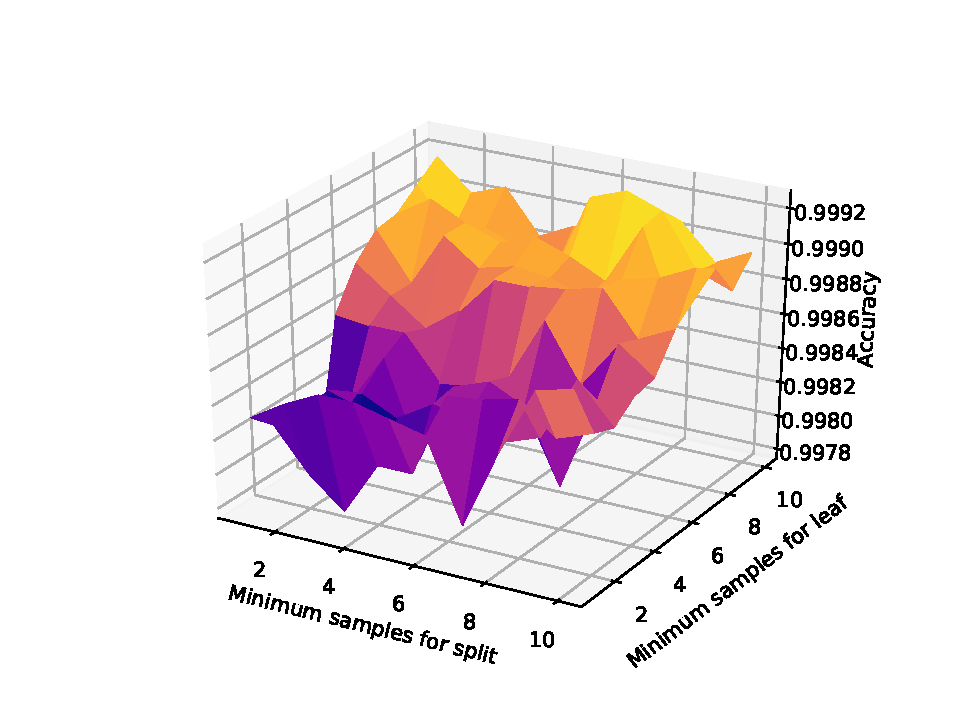
\includegraphics[width=0.5\textwidth]{nata/nata/DT/entropy_val}}
		
\subfloat[F1 score for gini criterion\label{nata-dt-f1-gini}]
		{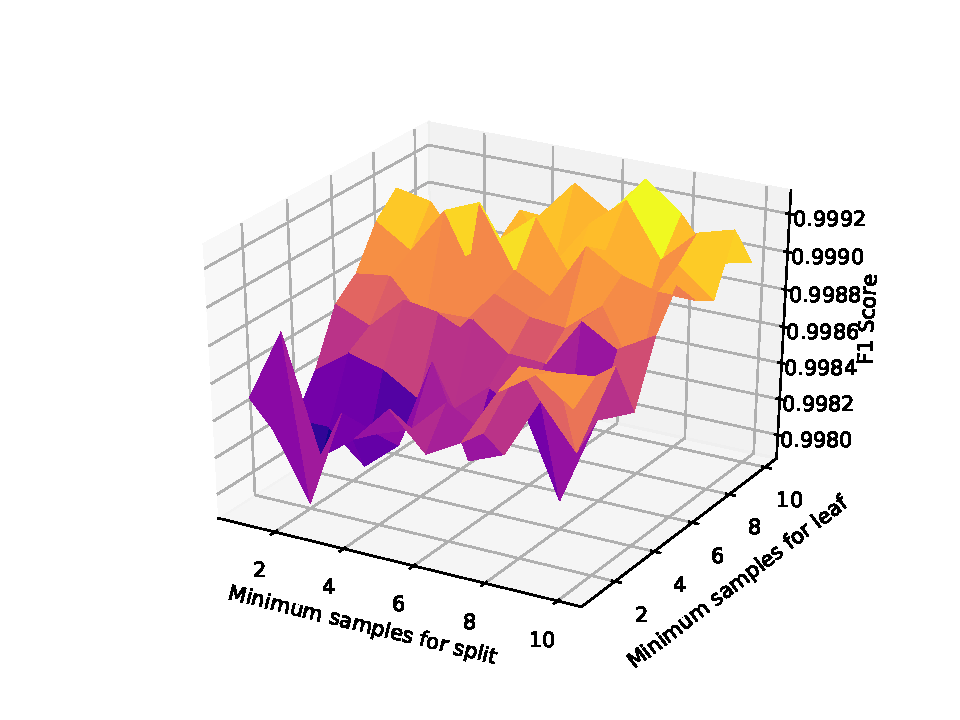
\includegraphics[width=0.5\textwidth]{nata/nata/DT/gini_f1}}
	\hfill	
\subfloat[F1 score for entropy criterion\label{nata-dt-f1-entropy}]
		{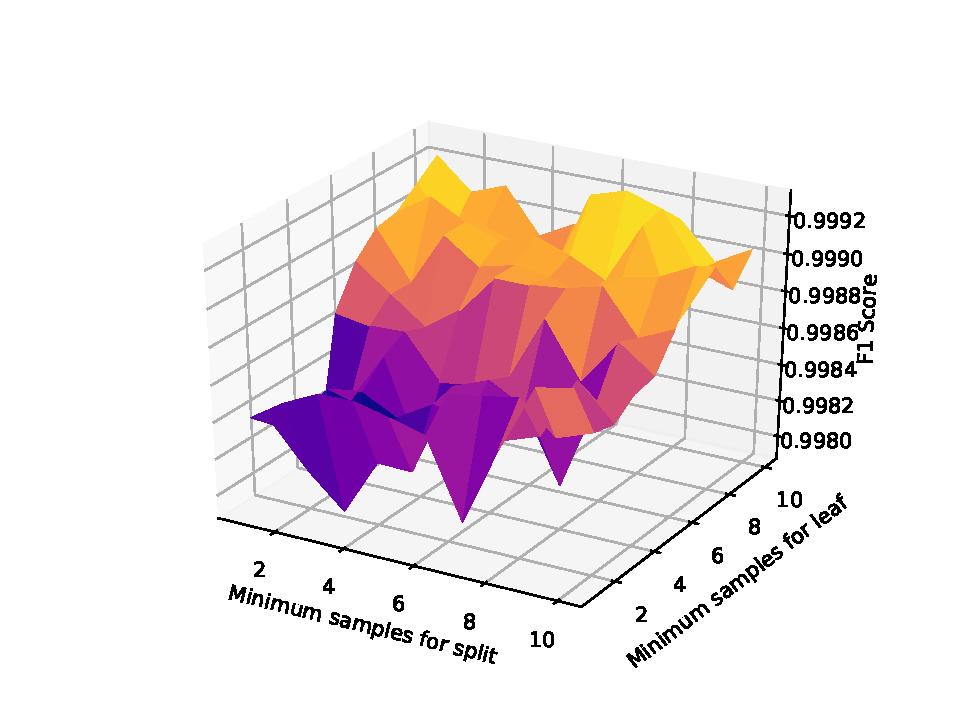
\includegraphics[width=0.5\textwidth]{nata/nata/DT/entropy_f1}}
		
\subfloat[Computational runtime for gini criterion\label{nata-dt-runtime-gini}]
		{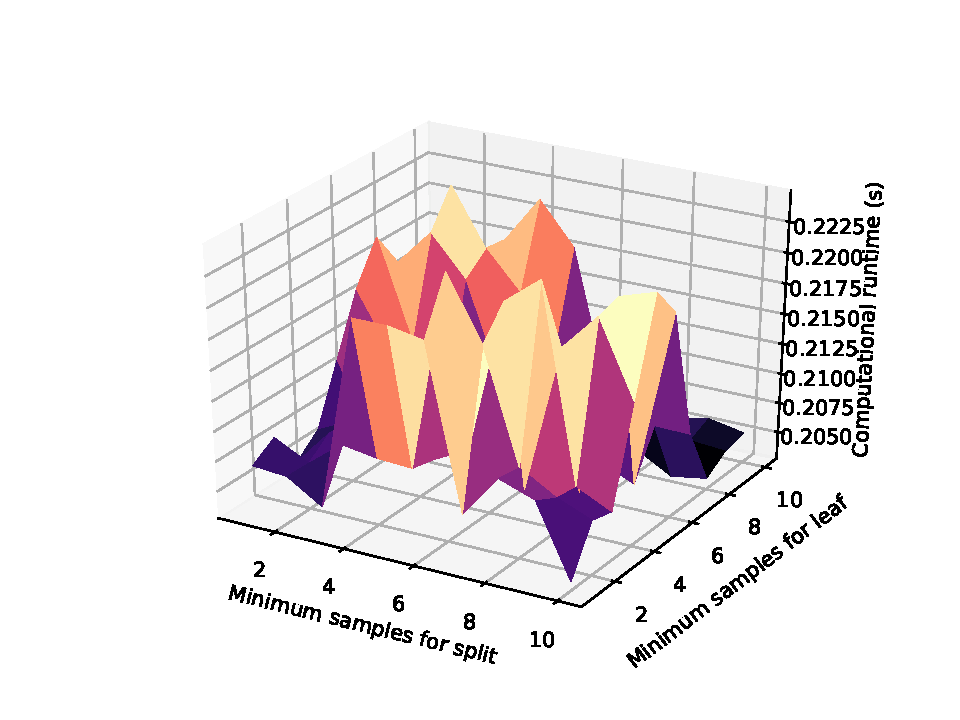
\includegraphics[width=0.5\textwidth]{nata/nata/DT/gini_runtime}}
	\hfill	
\subfloat[Computational runtime for entropy criterion\label{nata-dt-runtime-entropy}]
		{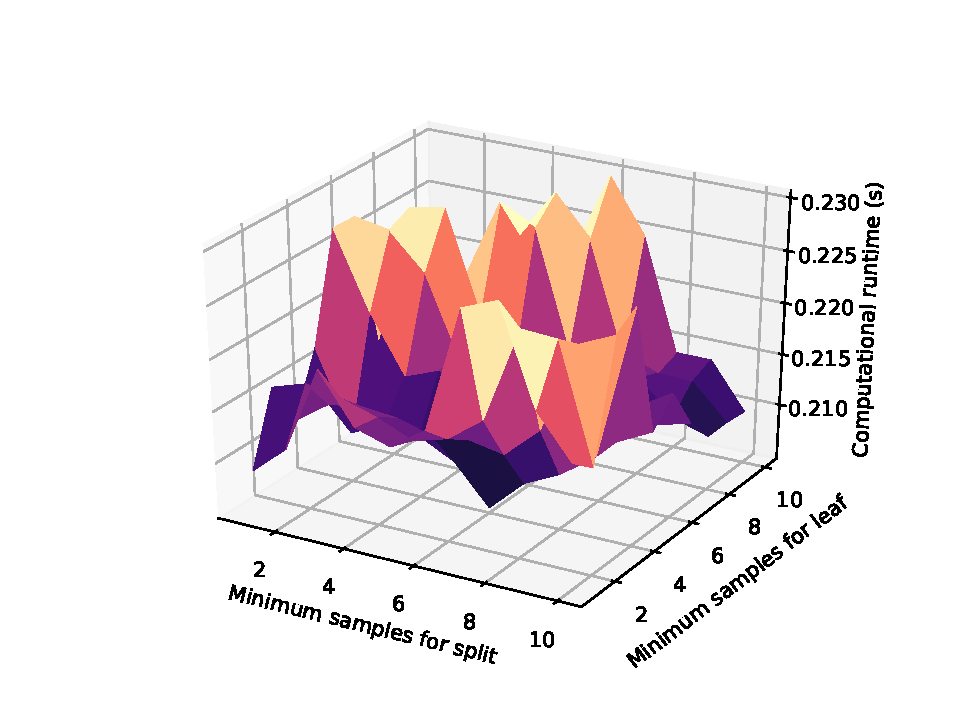
\includegraphics[width=0.5\textwidth]{nata/nata/DT/entropy_runtime}}
						
\caption{Plots of validation accuracy, F1 score, and computational runtime for DT on arithmetic data for gini and entropy criteria.}
	\label{dt-deap}
	\end{figure*}	

\begin{figure*}\centering
\subfloat[Validation error for gini criterion\label{nata-rfr-val-gini}]
		{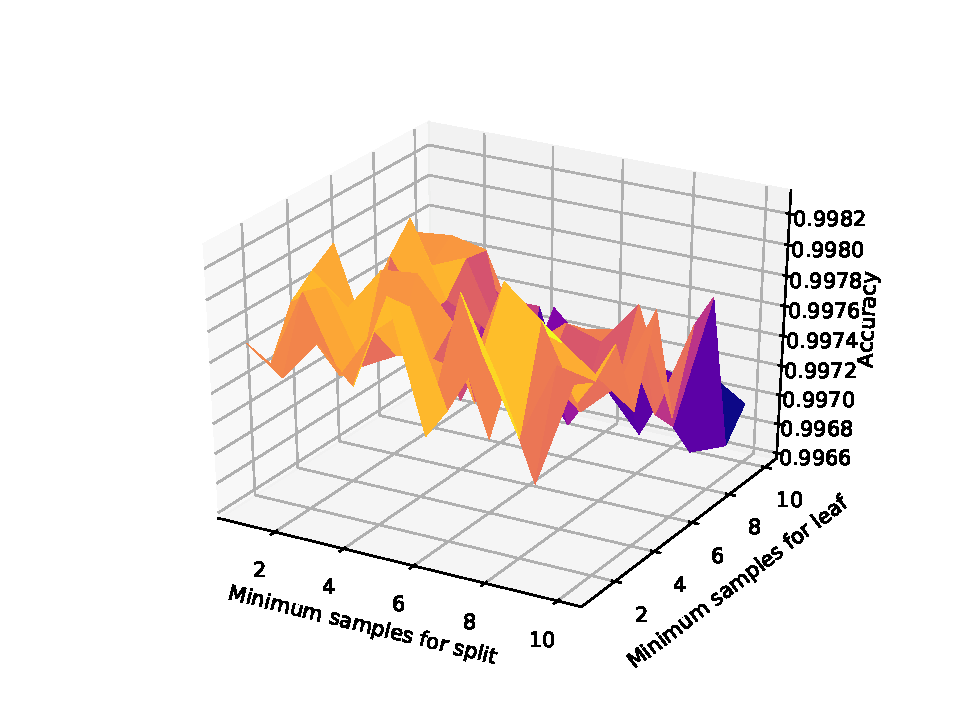
\includegraphics[width=0.5\textwidth]{nata/nata/RFR/gini_val}}
	\hfill	
\subfloat[Validation error for entropy criterion\label{nata-rfr-val-entropy}]
		{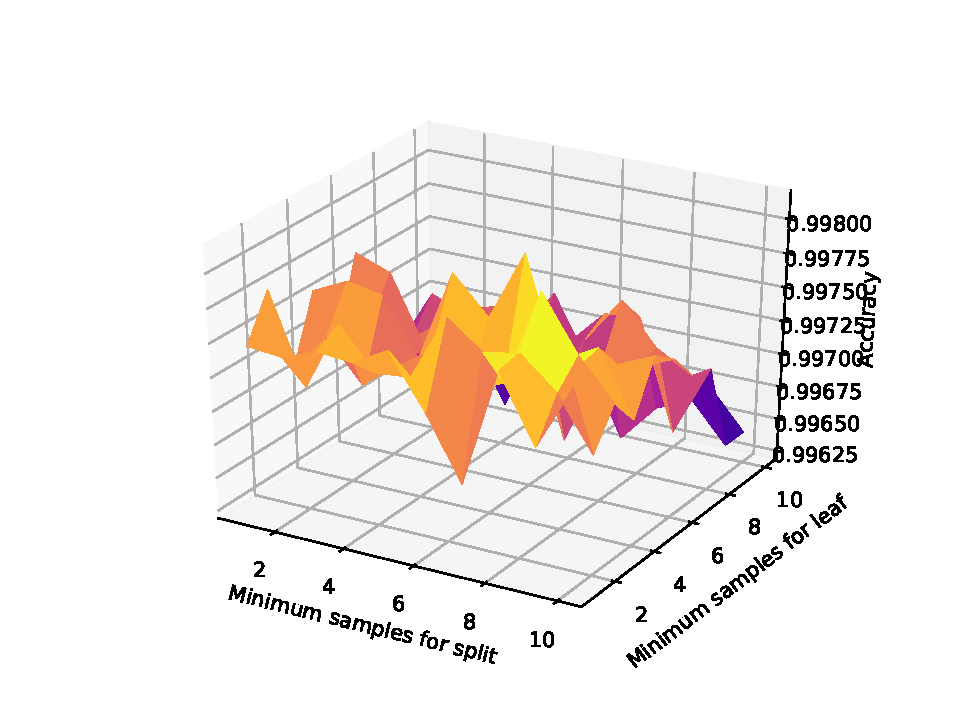
\includegraphics[width=0.5\textwidth]{nata/nata/RFR/entropy_val}}
		
\subfloat[F1 score for gini criterion\label{nata-rfr-f1-gini}]
		{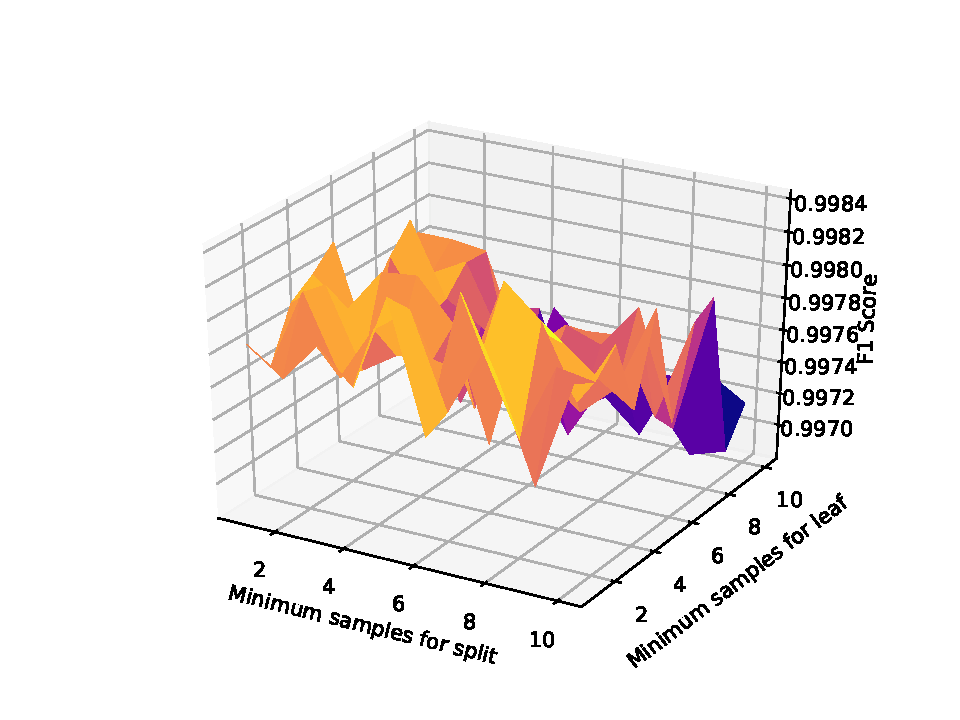
\includegraphics[width=0.5\textwidth]{nata/nata/RFR/gini_f1}}
	\hfill	
\subfloat[F1 score for entropy criterion\label{nata-rfr-f1-entropy}]
		{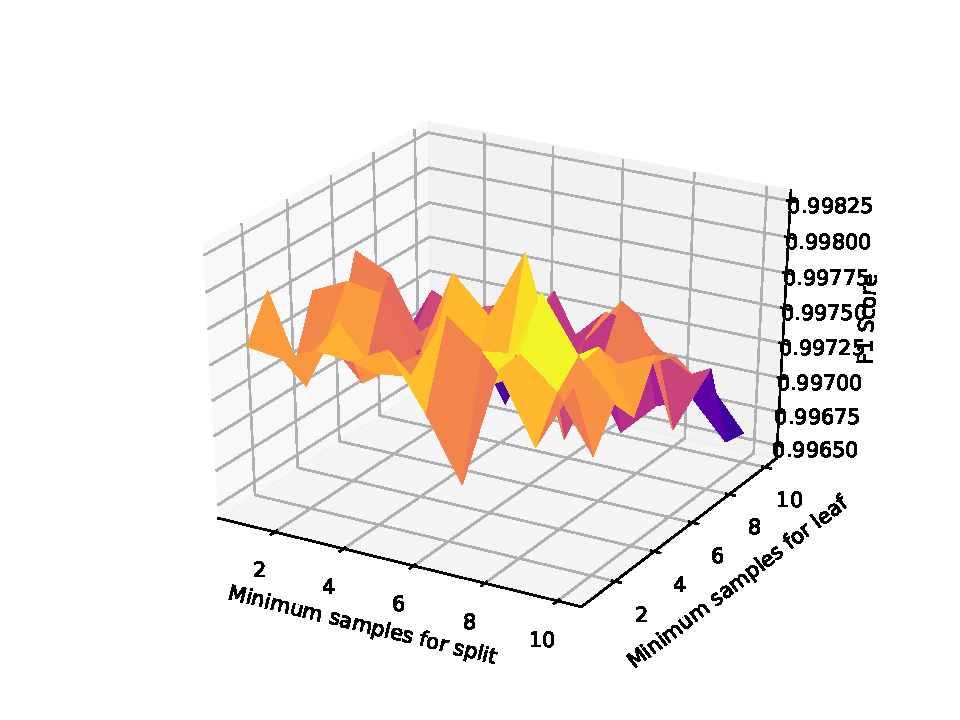
\includegraphics[width=0.5\textwidth]{nata/nata/RFR/entropy_f1}}
		
\subfloat[Computational runtime for gini criterion\label{nata-rfr-runtime-gini}]
		{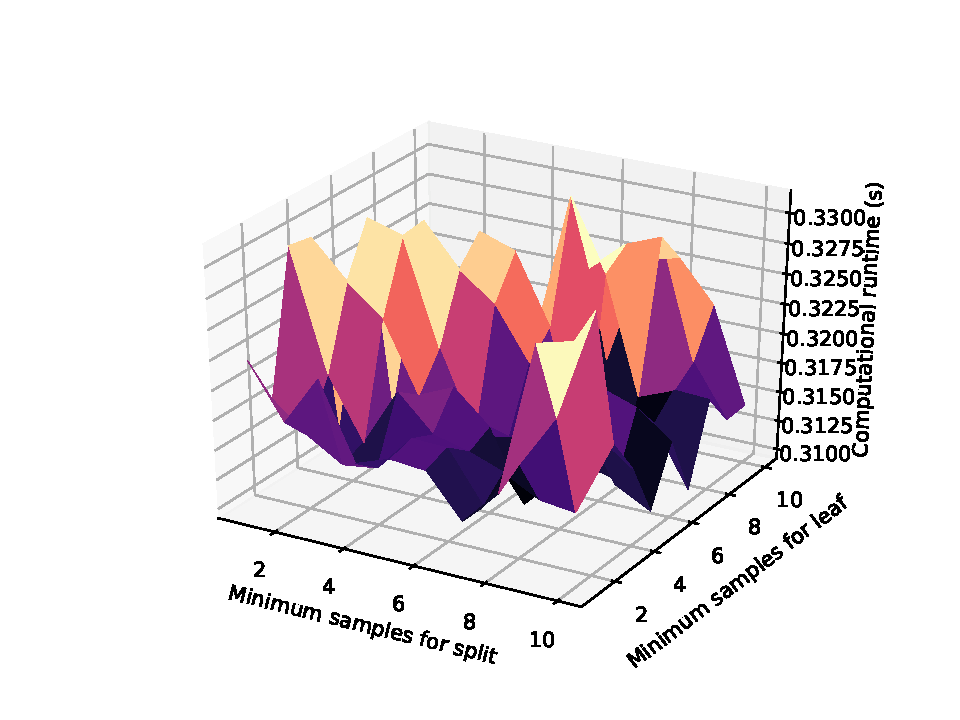
\includegraphics[width=0.5\textwidth]{nata/nata/RFR/gini_runtime}}
	\hfill	
\subfloat[Computational runtime for entropy criterion\label{nata-rfr-runtime-entropy}]
		{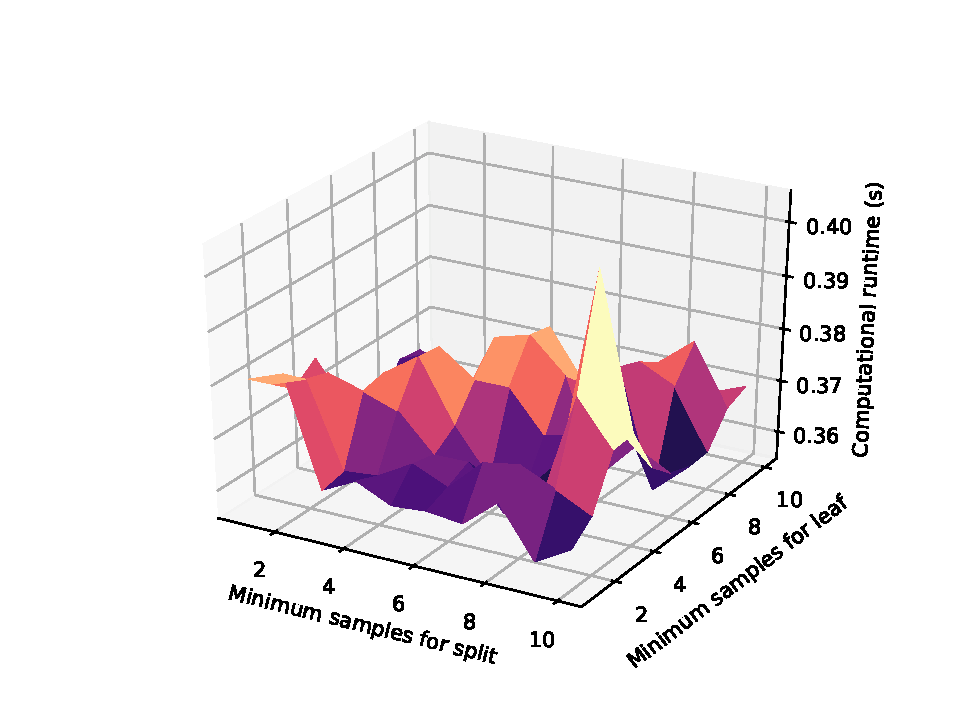
\includegraphics[width=0.5\textwidth]{nata/nata/RFR/entropy_runtime}}
						
\caption{Plots of validation accuracy, F1 score, and computational runtime for RF on arithmetic data for gini and entropy criteria.}
	\label{rfr-deap}
	\end{figure*}
	
Lastly, Figs.~\ref{dt-deap} and \ref{rfr-deap} provide the results for DT and RF, respectively. In both cases, accuracy and F1 score exceed .996 (or 99.6\%) under every variable combination. While there is very little variability in accuracy, it can be seen that accuracy varies proportionally with the minimum number of samples required for leaf under DT and slightly decreases with both variables under RF. Runtime varies by no more than 0.2 seconds and follows no noticeable patterns. 

\subsection{DEAP Emotion Recognition Dataset}

\begin{table}[!t]
\caption{Summary of training accuracy, validation accuracy, and computational runtime on DEAP data.}
\renewcommand{\arraystretch}{1.3}
\centering
%\resizebox{\textwidth}{!}
{\begin{tabular}{*{10}{l}}
\toprule
& \multicolumn{3}{l}{Train. Accuracy} & \multicolumn{3}{l}{Val. Accuracy} & \multicolumn{3}{l}{Runtime (s)} \\
Technique & Max & Min & Mean & Max & Min & Mean & Max & Min & Mean \\ \midrule
ANN SGD & .726 & .723 & .729 & .729 & .719 & .724 & 8.86 & 4.35 & 6.45 \\
ANN L-BFGS & .740 & .724 & .729 & .728 & .716 & .722 & 66.3 & 3.12 & 18.1 \\
KNN Uniform & 1.00 & .340 & .475 & .116 & .144 & .151 & 135 & 24.2 & 64.5 \\
KNN Distance & 1.00 & 1.00 & 1.00 & .165 & .154 & .160 & 116 & 15.4 & 50.2 \\
SVM Linear & .138 & .114 & .130 & .104 & .089 & .098 & 55.96 & 52.68 & 54.08 \\
SVM RBF & .982 & .217 & .785 & .174 & .129 & .165 & 92.7 & 70.5 & 84.9 \\
DT Gini & 1.00 & .491 & .642 & .179 & .170 & .175 & 19.8 & 13.6 & 16.6 \\
DT Entropy & 1.00 & .461 & .629 & .183 & .172 & .178 & 24.8 & 18.7 & 21.6 \\
RF Gini & .990 & .652 & .802 & .180 & .169 & .174 & 21.8 & 15.5 & 18.3 \\
RF Entropy & .990 & .658 & .805 & .178 & .165 & .173 & 24.5 & 18.8 & 21.4 \\ \bottomrule
\end{tabular}}

\label{tvr-deap}
\end{table}

Table \ref{tvr-deap} provides an overview of the accuracy and runtime results for the DEAP dataset in a manner similar to that of Table \ref{tvr-nata}. A key initial observation here is that no method under these experimental constraints is able to model the DEAP data as well as the arithmetic data. ANN is the only method with remotely acceptable results, with values ranging from 71.6\% to 72.9\%. With exception of the SVM linear kernel, which produced low training and validation accuracy just as it did in the previous dataset, all the remaining methods have been subjected to extreme cases of overfitting. This is evidenced by the high levels of training accuracy observed in many cases, which translated poorly into the validation stage. Another key observation is that runtime for this dataset was significantly longer than the previous one, which is most likely due to the increased number of inputs involved in this data. Hence, the minimum number of seconds required for an algorithmic instance is three seconds, while some maximums are as high as one-and-a-half minutes. Much like before, SVM consistently produces the highest amount of runtime, while ANN has the most variability. However, the latter case only holds true for the L-BFGS optimizer. In SGD, runtime is consistently the lowest while validation accuracy remains the highest. Thus, conclusions can be drawn so far that ANN under the SGD optimizer is the best choice out of the methods given for modeling the DEAP dataset.

\begin{table}[!t]
\caption{Summary of F1, precision, and recall scores on DEAP data.}
\renewcommand{\arraystretch}{1.3}
\centering
%\resizebox{\textwidth}{!}
{\begin{tabular}{*{10}{l}}
\toprule
& \multicolumn{3}{l}{F1} & \multicolumn{3}{l}{Precision} & \multicolumn{3}{l}{Recall} \\
Technique & Max & Min & Mean & Max & Min & Mean & Max & Min & Mean \\ \midrule
ANN SGD & .284 & .279 & .281 & .435 & .240 & .283 & .334 & .333 & .334 \\
ANN L-BFGS & .341 & .279 & .305 & .415 & .240 & .349 & .358 & .333 & .342 \\
KNN Uniform & .162 & .134 & .145 & .164 & .144 & .156 & .162 & .144 & .151 \\
KNN Distance & .164 & .153 & .159 & .165 & .154 & .160 & .165 & .153 & .160 \\
SVM Linear & .079 & .076 & .090 & .110 & .091 & .102 & .103 & .089 & .098 \\
SVM RBF & .173 & .123 & .163 & .175 & .140 & .166 & .174 & .130 & .165 \\
DT Gini & .178 & .169 & .173 & .180 & .171 & .175 & .179 & .171 & .175 \\
DT Entropy & .182 & .170 & .177 & .183 & .172 & .178 & .183 & .172 & .178 \\
RF Gini & .179 & .167 & .173 & .180 & .169 & .174 & .180 & .169 & .174 \\
RF Entropy & .176 & .161 & .171 & .178 & .167 & .173 & .178 & .165 & .173 \\ \bottomrule
\end{tabular}}

\label{fpr-deap}
\end{table}

A glance of the results under the remaining metrics is given in Table \ref{fpr-deap}. In a similar observation to that of the previous table, no method produces a particularly stellar score when compared to the arithmetic dataset. This includes ANN, although it still contains the highest values. Unlike validation accuracy, however, in which the method achieved modest values of over 70\%, its highest scores are no more than 0.435. It should be noted that the values of these metrics for all other methods are consistently lower than 0.2. Thus, if stellar modeling of the DEAP dataset was a higher priority in this research, better care would have to be taken to tune parameters and modify one or more of these methods to form more accurate and more effective classifications. Because the overall focus is on flight safety, however, doing so is of lesser importance and thus simply serves as a basis of comparison for the remainder of the experiment. 

\begin{figure*}\centering
\subfloat[Validation error for L-BFGS optimizer\label{deap-ann-val-lbfgs}]
		{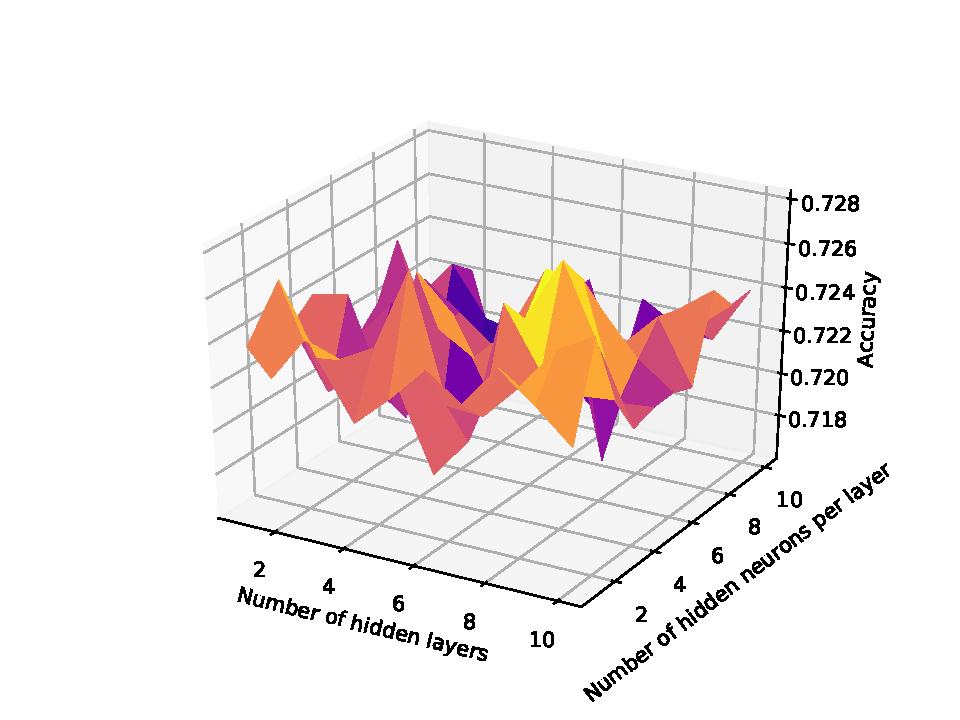
\includegraphics[width=0.5\textwidth]{deap/deap0/ANN/lbfgs_val}}
	\hfill	
\subfloat[Validation error for SGD optimizer\label{deap-ann-val-sgd}]
		{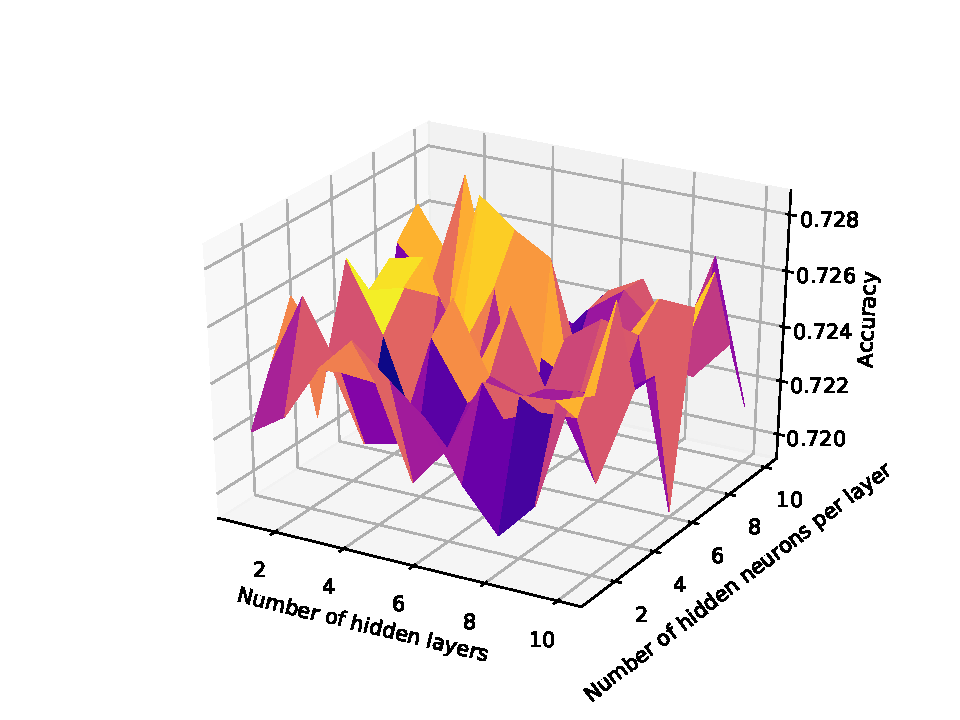
\includegraphics[width=0.5\textwidth]{deap/deap0/ANN/sgd_val}}
		
\subfloat[F1 score for L-BFGS optimizer\label{deap-ann-f1-lbfgs}]
		{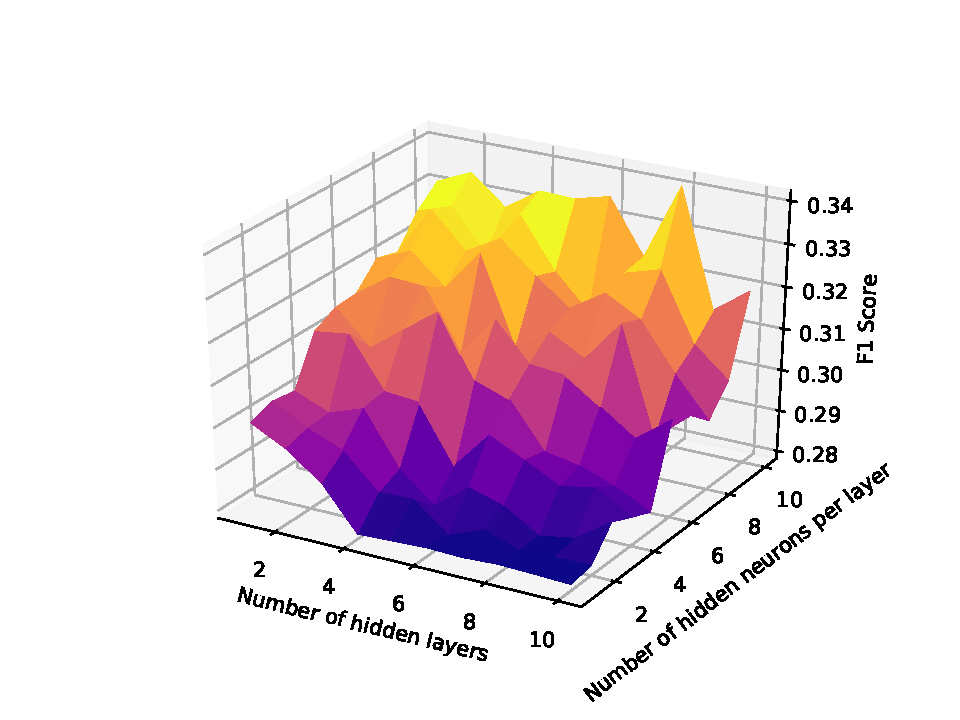
\includegraphics[width=0.5\textwidth]{deap/deap0/ANN/lbfgs_f1}}
	\hfill	
\subfloat[F1 score for SGD optimizer\label{deap-ann-f1-sgd}]
		{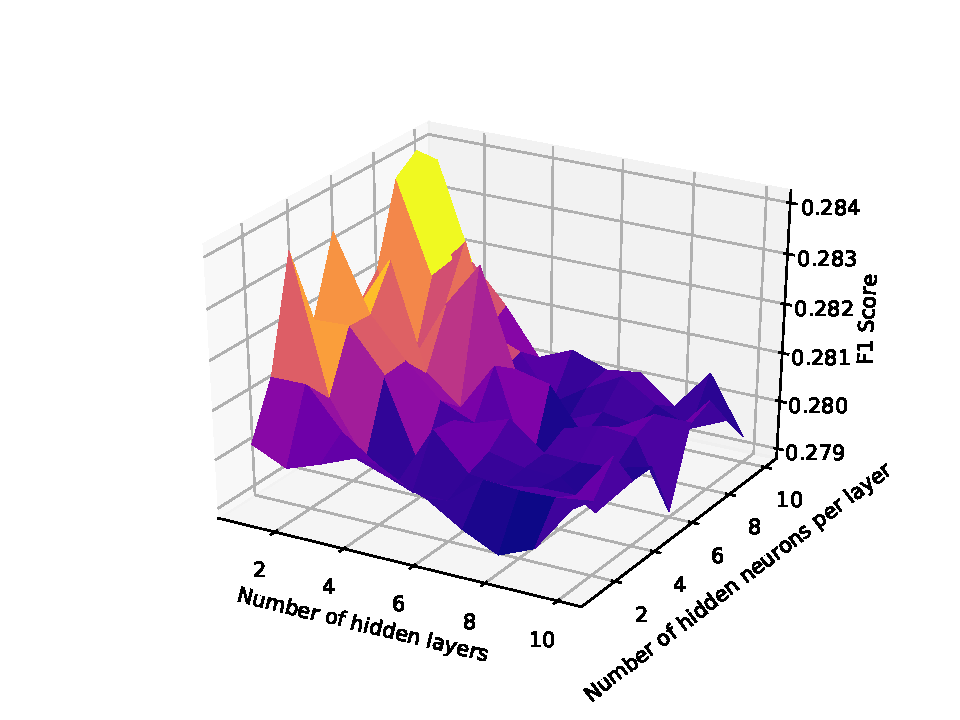
\includegraphics[width=0.5\textwidth]{deap/deap0/ANN/sgd_f1}}
		
\subfloat[Computational runtime for L-BFGS optimizer\label{deap-ann-runtime-lbfgs}]
		{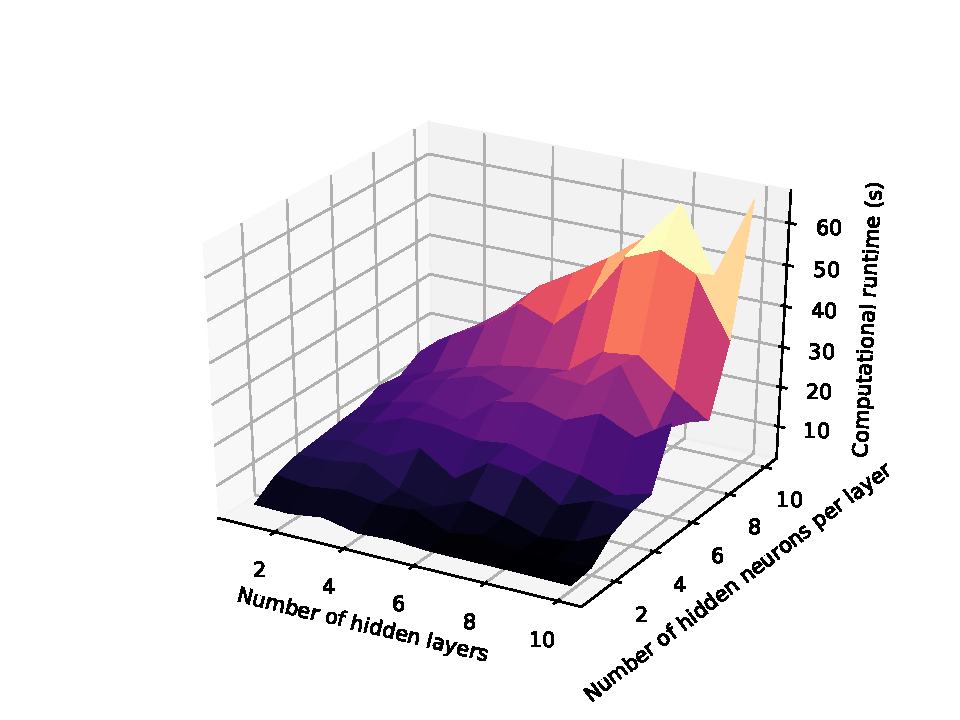
\includegraphics[width=0.5\textwidth]{deap/deap0/ANN/lbfgs_runtime}}
	\hfill	
\subfloat[Computational runtime for SGD optimizer\label{deap-ann-runtime-sgd}]
		{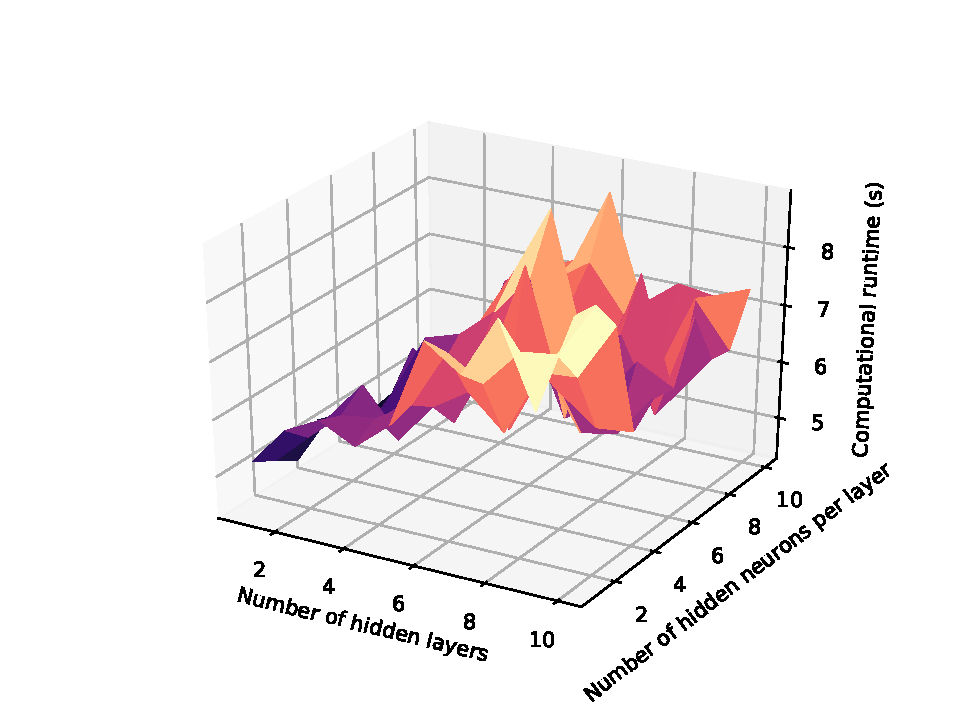
\includegraphics[width=0.5\textwidth]{deap/deap0/ANN/sgd_runtime}}
						
\caption{Plots of validation accuracy, F1 score, and computational runtime for ANN on DEAP data for L-BFGS and SGD optimizers.}
	\label{ann-deap}
	\end{figure*}

Upon taking a closer look at the results in a manner similar to that of the previous subsection, Fig.~\ref{ann-deap} presents graphical results of the ANN on the DEAP dataset. The most significant characteristic here is the fact that the validation error does not bear any resemblance to the F1 score, as was the case in the previous dataset. Here, the accuracy simply oscillates across a narrow range of values, while the F1 score forms a smoother surface. Under the L-BFGS optimizer, the F1 score follows a similar pattern to that of the previous data in which the score increases under an increase in number of hidden neurons and under a decrease of number of hidden layers. The SGD optimizer has the same trend for number of layers but no noticeable pattern for number of neurons. The computational runtime for L-BFGS increases proportionally with both axes and only with the number of layers for SGD. Like with the F1 score, there is no significant trend or pattern with the number of neurons in SGD. 

\begin{figure*}\centering
\subfloat[Validation error for linear kernel\label{deap-svm-val-linear}]
		{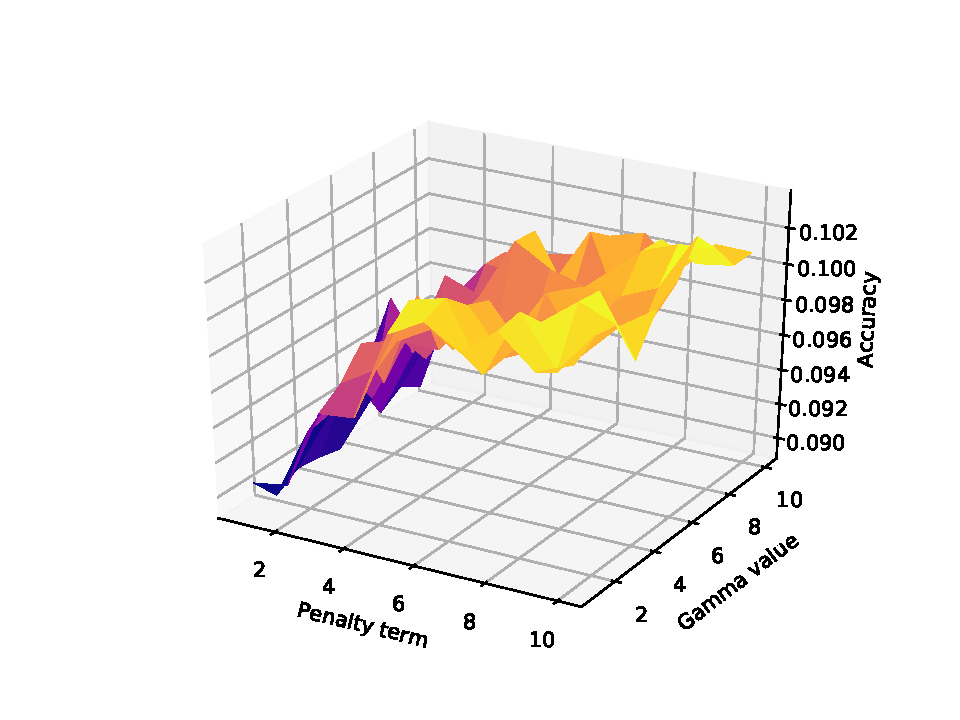
\includegraphics[width=0.5\textwidth]{deap/deap0/SVM/linear_val}}
	\hfill	
\subfloat[Validation error for RBF kernel\label{deap-svm-val-rbf}]
		{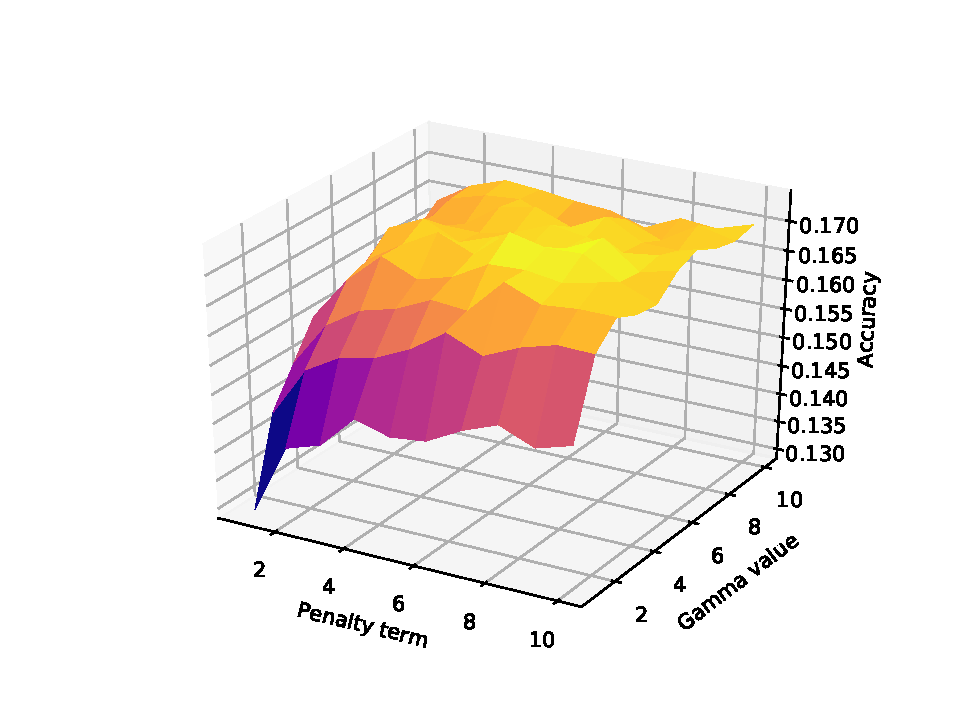
\includegraphics[width=0.5\textwidth]{deap/deap0/SVM/rbf_val}}
		
\subfloat[F1 score for linear kernel\label{deap-svm-f1-linear}]
		{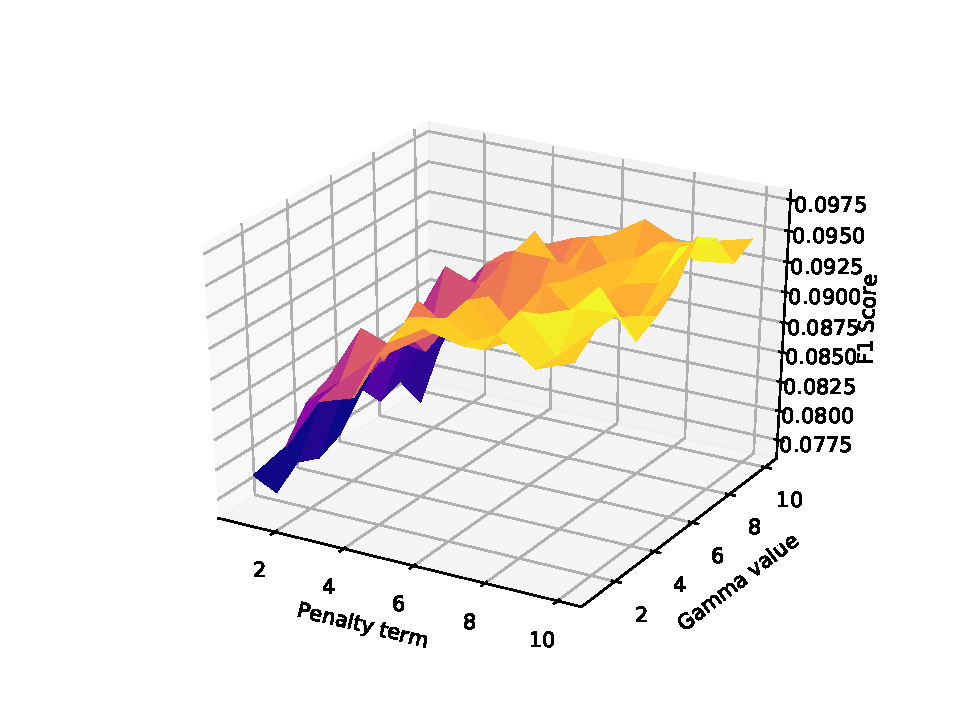
\includegraphics[width=0.5\textwidth]{deap/deap0/SVM/linear_f1}}
	\hfill	
\subfloat[F1 score for RBF kernel\label{deap-svm-f1-rbf}]
		{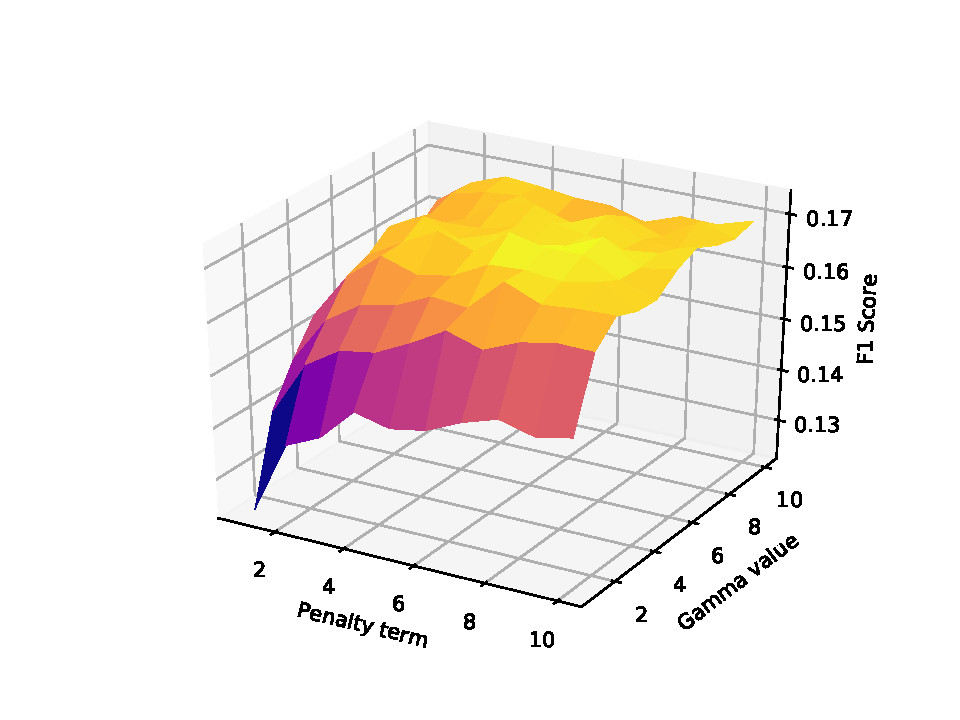
\includegraphics[width=0.5\textwidth]{deap/deap0/SVM/rbf_f1}}
		
\subfloat[Computational runtime for linear kernel\label{deap-svm-runtime-linear}]
		{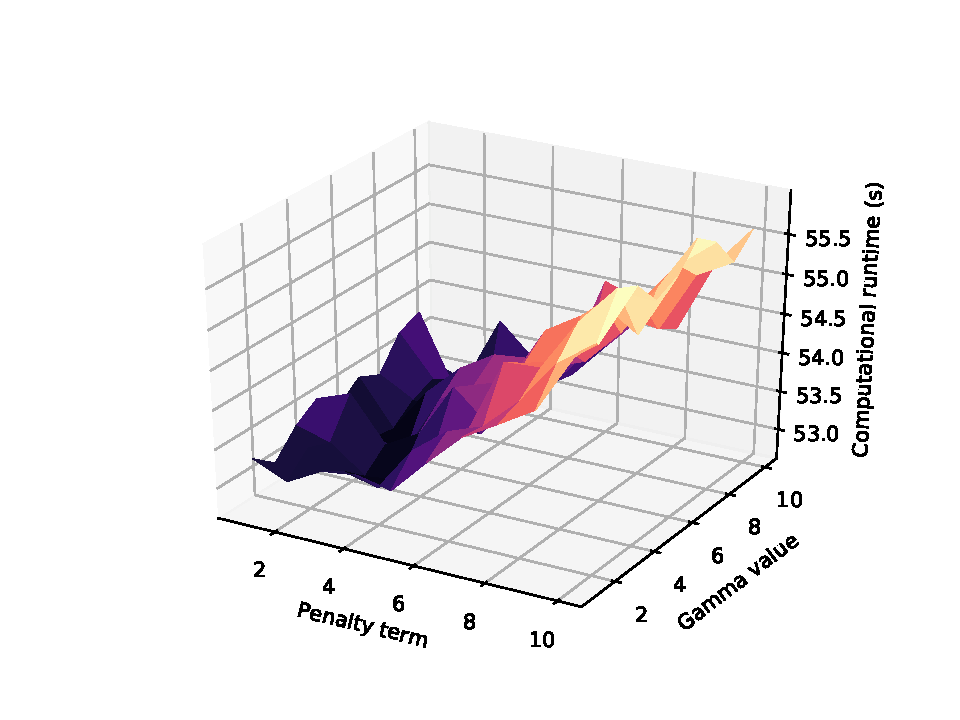
\includegraphics[width=0.5\textwidth]{deap/deap0/SVM/linear_runtime}}
	\hfill	
\subfloat[Computational runtime for linear kernel\label{deap-svm-runtime-rbf}]
		{\includegraphics[width=0.5\textwidth]{deap/deap0/SVM/rbf_runtime}}
						
\caption{Plots of validation accuracy, F1 score, and computational runtime for SVM on DEAP data for linear and RBF kernels.}
	\label{svm-deap}
	\end{figure*}
	
For the SVM results in Fig.~\ref{svm-deap}, validation error and F1 score once again share similar trends and values with one another. Despite containing significantly low values in these categories, the results under the RBF kernel bear similar patterns to the corresponding subfigures in the previous subsection, in which the metrics increase proportionally with both iterative parameters. Unlike before, however, these trends also apply to the linear kernel, although the corresponding curves are less smooth than their RBF counterparts. The runtime values, however, are drastically different from before. In this case, they more closely follow the accuracy and F1 plots in that runtime increases proportionally to each parameter. This once again varies between the two kernels in that RBF contains a smooth straightforward curve while linear is rougher and more oscillatory.

\begin{figure*}\centering
\subfloat[Validation error for uniform weights\label{deap-knn-val-uniform}]
		{\includegraphics[width=0.5\textwidth]{deap/deap0/KNN/uniform_val}}
	\hfill	
\subfloat[Validation error for distance weights\label{deap-knn-val-distance}]
		{\includegraphics[width=0.5\textwidth]{deap/deap0/KNN/distance_val}}
		
\subfloat[F1 score for uniform weights\label{deap-knn-f1-uniform}]
		{\includegraphics[width=0.5\textwidth]{deap/deap0/KNN/uniform_f1}}
	\hfill	
\subfloat[F1 score for distance weights\label{deap-knn-f1-distance}]
		{\includegraphics[width=0.5\textwidth]{deap/deap0/KNN/distance_f1}}
		
\subfloat[Computational runtime for uniform weights\label{deap-knn-runtime-uniform}]
		{\includegraphics[width=0.5\textwidth]{deap/deap0/KNN/uniform_runtime}}
	\hfill	
\subfloat[Computational runtime for distance weights\label{deap-knn-runtime-distance}]
		{\includegraphics[width=0.5\textwidth]{deap/deap0/KNN/distance_runtime}}
						
\caption{Plots of validation accuracy, F1 score, and computational runtime for KNN on DEAP data for uniform and distance weights.}
	\label{knn-deap}
	\end{figure*}

\begin{figure*}\centering
\subfloat[Validation error for gini criterion\label{deap-dt-val-gini}]
		{\includegraphics[width=0.5\textwidth]{deap/deap0/DT/gini_val}}
	\hfill	
\subfloat[Validation error for entropy criterion\label{deap-dt-val-entropy}]
		{\includegraphics[width=0.5\textwidth]{deap/deap0/DT/entropy_val}}
		
\subfloat[F1 score for gini criterion\label{deap-dt-f1-gini}]
		{\includegraphics[width=0.5\textwidth]{deap/deap0/DT/gini_f1}}
	\hfill	
\subfloat[F1 score for entropy criterion\label{deap-dt-f1-entropy}]
		{\includegraphics[width=0.5\textwidth]{deap/deap0/DT/entropy_f1}}
		
\subfloat[Computational runtime for gini criterion\label{deap-dt-runtime-gini}]
		{\includegraphics[width=0.5\textwidth]{deap/deap0/DT/gini_runtime}}
	\hfill	
\subfloat[Computational runtime for entropy criterion\label{deap-dt-runtime-entropy}]
		{\includegraphics[width=0.5\textwidth]{deap/deap0/DT/entropy_runtime}}
						
\caption{Plots of validation accuracy, F1 score, and computational runtime for DT on DEAP data for gini and entropy criteria.}
	\label{dt-deap}
	\end{figure*}

\begin{figure*}\centering
\subfloat[Validation error for gini criterion\label{deap-rfr-val-gini}]
		{\includegraphics[width=0.5\textwidth]{deap/deap0/RFR/gini_val}}
	\hfill	
\subfloat[Validation error for entropy criterion\label{deap-rfr-val-entropy}]
		{\includegraphics[width=0.5\textwidth]{deap/deap0/RFR/entropy_val}}
		
\subfloat[F1 score for gini criterion\label{deap-rfr-f1-gini}]
		{\includegraphics[width=0.5\textwidth]{deap/deap0/RFR/gini_f1}}
	\hfill	
\subfloat[F1 score for entropy criterion\label{deap-rfr-f1-entropy}]
		{\includegraphics[width=0.5\textwidth]{deap/deap0/RFR/entropy_f1}}
		
\subfloat[Computational runtime for gini criterion\label{deap-rfr-runtime-gini}]
		{\includegraphics[width=0.5\textwidth]{deap/deap0/RFR/gini_runtime}}
	\hfill	
\subfloat[Computational runtime for entropy criterion\label{deap-rfr-runtime-entropy}]
		{\includegraphics[width=0.5\textwidth]{deap/deap0/RFR/entropy_runtime}}
						
\caption{Plots of validation accuracy, F1 score, and computational runtime for RF on DEAP data for gini and entropy criteria.}
	\label{rfr-deap}
	\end{figure*}
	
Fig.~\ref{knn-deap} depicts the KNN results, in which accuracy and F1 score follow an oscillatory pattern within a highly narrow range of values for nearly all parameter combinations. The exception to this is under uniform weights when transitioning from one to two neighbors, in which there is a significant dip in accuracy. Such a significance, however, is merely relative to the range of values spanned by the remaining results, as the total difference in range is no more than .025, or 2.5\%. Figs.~\ref{dt-deap} and \ref{rfr-deap} provide the equivalent results for DT and RF, respectively. Overall, there is nothing significant to observe about these plots besides the fact that are highly among a relatively short range of values for each metric. Given that each of the metrics has been unsuccessful in modeling this dataset, no further elaboration is needed.

\subsection{EEG Visual Matching Dataset}

\begin{table}[!t]
\caption{Summary of training accuracy, validation accuracy, and computational runtime on visual matching data.}
\renewcommand{\arraystretch}{1.3}
\centering
%\resizebox{\textwidth}{!}
{\begin{tabular}{*{10}{l}}
\toprule
& \multicolumn{3}{l}{Train. Accuracy} & \multicolumn{3}{l}{Val. Accuracy} & \multicolumn{3}{l}{Runtime (s)} \\
Technique & Max & Min & Mean & Max & Min & Mean & Max & Min & Mean \\ \midrule
ANN SGD & .726 & .723 & .724 & .729 & .718 & .724 & 8.62 & 4.09 & 6.20 \\
ANN L-BFGS & .738 & .723 & .729 & .729 & .717 & .723 & 50.0 & 2.66 & 14.63 \\
KNN Uniform & 1.00 & .749 & .803 & .721 & .653 & .702 & 167 & 24.9 & 77.7 \\
KNN Distance & 1.00 & 1.00 & 1.00 & .716 & .655 & .693 & 161 & 23.4 & 74.5 \\
SVM Linear & .725 & .723 & .724 & .728 & .720 & .724 & 91.9 & 26.1 & 36.7 \\
SVM RBF & .999 & .735 & .935 & .738 & .702 & .723 & 181 & 60.8 & 138 \\
DT Gini & 1.00 & .944 & .960 & .932 & .889 & .915 & 29.8 & 19.7 & 25.3 \\
DT Entropy & 1.00 & .948 & .968 & .923 & .896 & .911 & 18.0 & 13.7 & 16.1 \\
RF Gini & .979 & .832 & .899 & .734 & .718 & .727 & 29.4 & 21.6 & 25.2 \\
RF Entropy & .978 & .843 & .912 & .733 & .718 & .727 & 18.9 & 13.5 & 16.2 \\ \bottomrule
\end{tabular}}

\label{tvr-vismatch}
\end{table}

A summary of the accuracy and runtime values for the visual matching data is presented in Table \ref{tvr-vismatch}. For the former category, results are significantly better than those of the DEAP dataset but not quite as high as in the arithmetic data. It is also worth noting that this is the first dataset in which the SVM linear kernel produces a minimally acceptable amount of accuracy, although in training it still produces the lowest range of accuracy values. In terms of training results, KNN under the distance weight configuration produces the best results possible, as every iterative parameter combination produces a perfect score. The next best training results stem from DT, as no validation value in this method falls below 90\%. It is also the only method in which both subjective parameter options produces 90\% training accuracy or better under all circumstances. Meanwhile, RF is the only other algorithm in which these results never drop below 80\%. ANN and SVM linear kernel perform the worst, as training values are consistently in the range of 72-74\%.

As for validation accuracy, DT is the only method with values above 74\%. On top of that, all of its values are also above 88\%, thereby easily making it the most ideal technique for accuracy alone in this dataset. For all the remaining methods, low validation accuracy was the result of either overfitting or similarly low training accuracy, depending on the parameters. Thus, conclusions can be reached that this data is easier to model than DEAP but more difficult than the arithmetic data. In terms of runtime, the best performance stemmed from ANN under the SGD optimizer. When coupled with mediocre accuracy, however, this trait is not particularly useful. The second best performer was a near tie between DT and RF. Given the high accuracy of DT, the former of the two methods is thereby observed to be the best balance so far of accuracy and runtime for this dataset.

\begin{table}[!t]
\caption{Summary of F1, precision, and recall scores on visual matching data.}
\renewcommand{\arraystretch}{1.3}
\centering
%\resizebox{\textwidth}{!}
{\begin{tabular}{*{10}{l}}
\toprule
& \multicolumn{3}{l}{F1} & \multicolumn{3}{l}{Precision} & \multicolumn{3}{l}{Recall} \\
Technique & Max & Min & Mean & Max & Min & Mean & Max & Min & Mean \\ \midrule
ANN SGD & .284 & .279 & .280 & .454 & .240 & .281 & .335 & .333 & .334 \\
ANN L-BFGS & .339 & .279 & .304 & .454 & .240 & .347 & .356 & .333 & .342 \\
KNN Uniform & .419 & .329 & .359 & .660 & .379 & .417 & .417 & .350 & .366 \\
KNN Distance & .417 & 353 & .379 & .640 & .384 & .417 & .416 & .361 & .380 \\
SVM Linear & .281 & .279 & .280 & .243 & .240 & .241 & .333 & .333 & .333 \\
SVM RBF & .423 & .290 & .376 & .643 & .407 & .497 & .405 & .337 & .378 \\
DT Gini & .631 & .590 & .605 & .681 & .594 & .618 & .621 & .588 & .600 \\
DT Entropy & .619 & .585 & .602 & .638 & .585 & .606 & .621 & .585 & .600 \\
RF Gini & .363 & .335 & .350 & .438 & .400 & .421 & .369 & .356 & .363 \\
RF Entropy & .363 & .335 & .350 & .438 & .400 & .421 & .369 & .356 & .363 \\ \bottomrule
\end{tabular}}

\label{fpr-vismatch}
\end{table}

When observing similarly organized results for the other three metrics in Table \ref{fpr-vismatch}, a stark difference is that none of the F1, precision, or recall results closely resemble the accuracy results, as was the case in many aspects of the previous two datasets. DT once again produces the highest scores across the board, but there is still a significant drop from accuracy values. This is likely due to the increased complexity of the data when compared to the arithmetic dataset. For all other methods, scores ranged anywhere from .240 to .660.

\begin{figure*}\centering
\subfloat[Validation error for L-BFGS optimizer\label{vismatch-ann-val-lbfgs}]
		{\includegraphics[width=0.5\textwidth]{vismatch1/vismatch0/ANN/lbfgs_val}}
	\hfill	
\subfloat[Validation error for SGD optimizer\label{vismatch-ann-val-sgd}]
		{\includegraphics[width=0.5\textwidth]{vismatch1/vismatch0/ANN/sgd_val}}
		
\subfloat[F1 score for L-BFGS optimizer\label{vismatch-ann-f1-lbfgs}]
		{\includegraphics[width=0.5\textwidth]{vismatch1/vismatch0/ANN/lbfgs_f1}}
	\hfill	
\subfloat[F1 score for SGD optimizer\label{vismatch-ann-f1-sgd}]
		{\includegraphics[width=0.5\textwidth]{vismatch1/vismatch0/ANN/sgd_f1}}
		
\subfloat[Computational runtime for L-BFGS optimizer\label{vismatch-ann-runtime-lbfgs}]
		{\includegraphics[width=0.5\textwidth]{vismatch1/vismatch0/ANN/lbfgs_runtime}}
	\hfill	
\subfloat[Computational runtime for SGD optimizer\label{vismatch-ann-runtime-sgd}]
		{\includegraphics[width=0.5\textwidth]{vismatch1/vismatch0/ANN/sgd_runtime}}
						
\caption{Plots of validation accuracy, F1 score, and computational runtime for ANN on visual matching data for L-BFGS and SGD optimizers.}
	\label{ann-vismatch}
	\end{figure*}

\begin{figure*}\centering
\subfloat[Validation error for linear kernel\label{vismatch-svm-val-linear}]
		{\includegraphics[width=0.5\textwidth]{vismatch1/vismatch0/SVM/linear_val}}
	\hfill	
\subfloat[Validation error for RBF kernel\label{vismatch-svm-val-rbf}]
		{\includegraphics[width=0.5\textwidth]{vismatch1/vismatch0/SVM/rbf_val}}
		
\subfloat[F1 score for linear kernel\label{vismatch-svm-f1-linear}]
		{\includegraphics[width=0.5\textwidth]{vismatch1/vismatch0/SVM/linear_f1}}
	\hfill	
\subfloat[F1 score for RBF kernel\label{vismatch-svm-f1-rbf}]
		{\includegraphics[width=0.5\textwidth]{vismatch1/vismatch0/SVM/rbf_f1}}
		
\subfloat[Computational runtime for linear kernel\label{vismatch-svm-runtime-linear}]
		{\includegraphics[width=0.5\textwidth]{vismatch1/vismatch0/SVM/linear_runtime}}
	\hfill	
\subfloat[Computational runtime for linear kernel\label{vismatch-svm-runtime-rbf}]
		{\includegraphics[width=0.5\textwidth]{vismatch1/vismatch0/SVM/rbf_runtime}}
						
\caption{Plots of validation accuracy, F1 score, and computational runtime for SVM on visual matching data for linear and RBF kernels.}
	\label{svm-vismatch}
	\end{figure*}
	
Figs.~\ref{ann-vismatch} and \ref{svm-vismatch} contain this dataset's graphical results for ANN and SVM, respectively. For the ANN results, despite drastically different ranges of values, every pattern and trend observed in Fig.~\ref{ann-deap} holds true for every respective subfigure of Fig.~\ref{ann-vismatch}. The only real change is that all the corresponding metric values are simply better. The SVM results, however, are drastically different from their DEAP counterparts. In the linear kernel, the validation error and F1 score plots closely resemble each other in that there is no noticeable pattern along the axes, just more oscillation among a narrow range of values. In the RBF kernel, the plots for the same two metrics are widely different from one another. Validation error appears to decrease as the penalty term increases, while the gamma value causes the function to decrease to a minimum when reaching a gamma value of five, then increases afterwards, essentially creating a valley area in the surface. The F1 score, however, follows a completely inverse trend, in which the score increases proportionally with the penalty term and a peak exists along the gamma value axis. As for runtime, the linear kernel contains a more unusual surface in which runtime is below 30 seconds and slowly increases along the x axis  until the penalty term reaches eight, at which point the slop increases drastically. Meanwhile, changes in gamma values seem to have to no effect on this metric. The linear kernel, however, produces a smooth surface with correlations closely resembling those of the F1 score but over a wider range of values, spanning from 60 to 190 seconds.

\begin{figure*}\centering
\subfloat[Validation error for uniform weights\label{vismatch-knn-val-uniform}]
		{\includegraphics[width=0.5\textwidth]{vismatch2/vismatch0/KNN/uniform_val}}
	\hfill	
\subfloat[Validation error for distance weights\label{vismatch-knn-val-distance}]
		{\includegraphics[width=0.5\textwidth]{vismatch2/vismatch0/KNN/distance_val}}
		
\subfloat[F1 score for uniform weights\label{vismatch-knn-f1-uniform}]
		{\includegraphics[width=0.5\textwidth]{vismatch2/vismatch0/KNN/uniform_f1}}
	\hfill	
\subfloat[F1 score for distance weights\label{vismatch-knn-f1-distance}]
		{\includegraphics[width=0.5\textwidth]{vismatch2/vismatch0/KNN/distance_f1}}
		
\subfloat[Computational runtime for uniform weights\label{vismatch-knn-runtime-uniform}]
		{\includegraphics[width=0.5\textwidth]{vismatch2/vismatch0/KNN/uniform_runtime}}
	\hfill	
\subfloat[Computational runtime for distance weights\label{vismatch-knn-runtime-distance}]
		{\includegraphics[width=0.5\textwidth]{vismatch2/vismatch0/KNN/distance_runtime}}
						
\caption{Plots of validation accuracy, F1 score, and computational runtime for KNN on visual matching data for uniform and distance weights.}
	\label{knn-vismatch}
	\end{figure*}
	
The KNN results in Fig.~\ref{knn-vismatch} present some more stark differences between validation accuracy and F1 score but similar trends between weight configurations. Under both metrics, however, the only common observation is that changes in the leaf size does not appear to impact the respective metrics. Accuracy appears to vary proportionally with the number of neighbors but with some oscillation. This oscillation is greater and more noticeable with uniform weights than it is with distance weights. The F1 score, however, varies inversely with the number of neighbors under both weight configurations. The runtime under both scenarios appears to be almost exactly the same under both uniform and distance weights, although there are in fact some slight numerical differences. In this metric, runtime decreases noticeably with leaf size and increases slightly with number of neighbors.

\begin{figure*}\centering
\subfloat[Validation error for gini criterion\label{vismatch-dt-val-gini}]
		{\includegraphics[width=0.5\textwidth]{vismatch2/vismatch0/DT/gini_val}}
	\hfill	
\subfloat[Validation error for entropy criterion\label{vismatch-dt-val-entropy}]
		{\includegraphics[width=0.5\textwidth]{vismatch2/vismatch0/DT/entropy_val}}
		
\subfloat[F1 score for gini criterion\label{vismatch-dt-f1-gini}]
		{\includegraphics[width=0.5\textwidth]{vismatch2/vismatch0/DT/gini_f1}}
	\hfill	
\subfloat[F1 score for entropy criterion\label{vismatch-dt-f1-entropy}]
		{\includegraphics[width=0.5\textwidth]{vismatch2/vismatch0/DT/entropy_f1}}
		
\subfloat[Computational runtime for gini criterion\label{vismatch-dt-runtime-gini}]
		{\includegraphics[width=0.5\textwidth]{vismatch2/vismatch0/DT/gini_runtime}}
	\hfill	
\subfloat[Computational runtime for entropy criterion\label{vismatch-dt-runtime-entropy}]
		{\includegraphics[width=0.5\textwidth]{vismatch2/vismatch0/DT/entropy_runtime}}
						
\caption{Plots of validation accuracy, F1 score, and computational runtime for DT on visual matching data for gini and entropy criteria.}
	\label{dt-vismatch}
	\end{figure*}

\begin{figure*}\centering
\subfloat[Validation error for gini criterion\label{vismatch-rfr-val-gini}]
		{\includegraphics[width=0.5\textwidth]{vismatch2/vismatch0/RFR/gini_val}}
	\hfill	
\subfloat[Validation error for entropy criterion\label{vismatch-rfr-val-entropy}]
		{\includegraphics[width=0.5\textwidth]{vismatch2/vismatch0/RFR/entropy_val}}
		
\subfloat[F1 score for gini criterion\label{vismatch-rfr-f1-gini}]
		{\includegraphics[width=0.5\textwidth]{vismatch2/vismatch0/RFR/gini_f1}}
	\hfill	
\subfloat[F1 score for entropy criterion\label{vismatch-rfr-f1-entropy}]
		{\includegraphics[width=0.5\textwidth]{vismatch2/vismatch0/RFR/entropy_f1}}
		
\subfloat[Computational runtime for gini criterion\label{vismatch-rfr-runtime-gini}]
		{\includegraphics[width=0.5\textwidth]{vismatch2/vismatch0/RFR/gini_runtime}}
	\hfill	
\subfloat[Computational runtime for entropy criterion\label{vismatch-rfr-runtime-entropy}]
		{\includegraphics[width=0.5\textwidth]{vismatch2/vismatch0/RFR/entropy_runtime}}
						
\caption{Plots of validation accuracy, F1 score, and computational runtime for RF on visual matching data for gini and entropy criteria.}
	\label{rfr-vismatch}
	\end{figure*}	
	
Finally, Figs.~\ref{dt-vismatch} and \ref{rfr-vismatch} depict the results for DT and RF, respectively. In both methods in each subjective parameter, validation error increases proportionally with the minimum number of samples for leaf, while the minimum number of samples for split have no noticeable correlation. The only notable difference between the plots for DT and RF is that the surfaces of the former are smoother and have less oscillation than the latter, particularly when compared to RF under the entropy criterion. The F1 score, however, varies substantially from method to method but not from criterion to criterion. In DT, there are no noticeable trends upon variation of the axes, whereas in RF, the score varies inversely with the minimum number of samples for leaf. Changes in the minimum samples for split, however, does not seem to affect the outcome. Meanwhile, computational runtime in all four cases has no real correlation with the x or y axis values, just oscillations among 4-10 second ranges of values.

\subsection{SAPHYRE Pilot Dataset}

\begin{table}[!t]
\caption{Summary of training accuracy, validation accuracy, and computational runtime on SAPHYRE data.}
\renewcommand{\arraystretch}{1.3}
\centering
%\resizebox{\textwidth}{!}
{\begin{tabular}{*{10}{l}}
\toprule
& \multicolumn{3}{l}{Train. Accuracy} & \multicolumn{3}{l}{Val. Accuracy} & \multicolumn{3}{l}{Runtime (s)} \\
Technique & Max & Min & Mean & Max & Min & Mean & Max & Min & Mean \\ \midrule
ANN SGD & .932 & .080 & .567 & .930 & .080 & .565 & 66.2 & 9.69 & 28.0 \\ 
ANN L-BFGS & .981 & .081 & .514 & .973 & .079 & .511 & 137 & 3.88 & 69.3 \\ 
KNN Uniform & 1.00 & .963 & .980 & .984 & .949 & .966 & 15.1 & 7.24 & 10.2 \\
KNN Distance & 1.00 & 1.00 & 1.00 & .984 & .970 & .977 & 14.7 & 5.99 & 9.09 \\
SVM Linear & .971 & .948 & .964 & .967 & .944 & .960 & 12.2 & 8.30 & 9.47 \\
SVM RBF & .999 & .978 & .995 & .986 & .972 & .981 & 53.6 & 16.6 & 34.7 \\
DT Gini & 1.00 & .991 & .995 & .993 & .984 & .989 & 10.7 & 6.62 & 8.34 \\
DT Entropy & 1.00 & .991 & .995 & .993 & .984 & .989 & 9.07 & 6.27 & 7.59 \\
RF Gini & 1.00 & .994 & .997 & .995 & .987 & .992 & 11.4 & 6.77 & 9.03 \\
RF Entropy & 1.00 & .995 & .998 & .995 & .989 & .993 & 10.3 & 6.51 & 8.42 \\ \bottomrule
\end{tabular}}

\label{tvr-saphyre}
\end{table}

Finally, the remainder of results left to observe involve the dataset of greatest importance to this chapter, the SAPHYRE dataset. This is because SAPHYRE is the only dataset to involve pilots, thereby containing the greatest relevance to the overarching dissertation topic of flight safety as well as to the current phase of the research based specifically on manned flight safety. Therefore, the successful ability to model this dataset under any of the ongoing experimental parameters is this chapter's highest priority.

Following the same pattern as in the previous three subsections, an overview of the runtime and accuracy results is given in Table \ref{tvr-saphyre}. In terms of training accuracy, every method besides ANN produces consistently high accuracy, in that no training accuracy value is below 94\%. Another unique trend is that for three of the five methods, the maximum training accuracy reached is a perfect score. In addition, KNN under distance weights results in a perfect training score for every iterative parameter combination. In this data, ANN carries the distinction of having substantially high and substantially low accuracy values, ranging anywhere from 8\% to 98\%.

Turning to validation accuracy, the overall values for each method held up quite well. As the respective columns indicate, there is not a single trace of overfitting. Overall, RF produces the highest possible accuracy values as well as the highest minimum and average values. DT is a close second, followed by a near tie between KNN and SVM. ANN still produces a relatively high maximum value but still spans a wide range of results, this time varying from 8\% to 93\%. 

In terms of computational runtime, ANN produces the maximum possible runtime as well as the minimum, continuing the trend so far of overwhelmingly wide metric ranges for ANN in this dataset. SVM has the second highest maximum value, while KNN has the second lowest minimum value. As for entire ranges of runtime results, DT produces the lowest, while SVM produces the highest. Overall so far, conclusions can be made that RF is the best method for accuracy, while DT is most ideal for speed and efficiency. In terms of optimal balance of speed and accuracy, DT has a slightly greater balance, although RF is a highly close second.

\begin{table}[!t]
\caption{Summary of F1, precision, and recall scores on SAPHYRE data.}
\renewcommand{\arraystretch}{1.3}
\centering
%\resizebox{\textwidth}{!}
{\begin{tabular}{*{10}{l}}
\toprule
& \multicolumn{3}{l}{F1} & \multicolumn{3}{l}{Precision} & \multicolumn{3}{l}{Recall} \\
Technique & Max & Min & Mean & Max & Min & Mean & Max & Min & Mean \\ \midrule
ANN SGD & .865 & .004 & .429 & .880 & .002 & .437 & .865 & .027 & .451 \\ 
ANN L-BFGS & .962 & .004 & .376 & .964 & .002 & .378 & .961 & .027 & .401 \\ 
KNN Uniform & .981 & .940 & .959 & .981 & .947 & .963 & .981 & .935 & .956 \\
KNN Distance & .981 & .965 & .973 & .982 & .967 & .975 & .981 & .963 & .972 \\
SVM Linear & .953 & .906 & .940 & .959 & .930 & .950 & .950 & .904 & .937 \\
SVM RBF & .984 & .968 & .977 & .985 & .971 & .982 & .983 & .960 & .973 \\
DT Gini & .991 & .976 & .982 & .992 & .976 & .984 & .991 & .976 & .982 \\
DT Entropy & .991 & .975 & .984 & .991 & .976 & .985 & .991 & .975 & .984 \\
RF Gini & .992 & .982 & .988 & .994 & .986 & .990 & .991 & .979 & .986 \\
RF Entropy & .993 & .983 & .989 & .994 & .987 & .991 & .992 & .979 & .987 \\ \bottomrule
\end{tabular}}

\label{fpr-saphyre}
\end{table}

When observing the F1, precision, and runtime results in Table \ref{fpr-saphyre}, ANN continues its tend of wide ranges of results, as its F1 score varies from 0.004 to 0.865, precision ranges from .002 to .880, and recall varies slightly less drastically from .027 to .865. In all three metrics, RF excels at all three with the best maximum, minimum, and average values for each category. SVM under the linear kernel has the consistently worst values, while DT has the second best. Thus, when identifying the most ideal method for the SAPHYRE data under all six metrics, RF has the best balance of all six result categories, while DT is the slightly balance of accuracy and runtime alone.

\begin{figure*}\centering
\subfloat[Validation error for L-BFGS optimizer\label{saphyre-ann-val-lbfgs}]
		{\includegraphics[width=0.5\textwidth]{saphyre/ANN/lbfgs_val}}
	\hfill	
\subfloat[Validation error for SGD optimizer\label{saphyre-ann-val-sgd}]
		{\includegraphics[width=0.5\textwidth]{saphyre/ANN/sgd_val}}
		
\subfloat[F1 score for L-BFGS optimizer\label{saphyre-ann-f1-lbfgs}]
		{\includegraphics[width=0.5\textwidth]{saphyre/ANN/lbfgs_f1}}
	\hfill	
\subfloat[F1 score for SGD optimizer\label{saphyre-ann-f1-sgd}]
		{\includegraphics[width=0.5\textwidth]{saphyre/ANN/sgd_f1}}
		
\subfloat[Computational runtime for L-BFGS optimizer\label{saphyre-ann-runtime-lbfgs}]
		{\includegraphics[width=0.5\textwidth]{saphyre/ANN/lbfgs_runtime}}
	\hfill	
\subfloat[Computational runtime for SGD optimizer\label{saphyre-ann-runtime-sgd}]
		{\includegraphics[width=0.5\textwidth]{saphyre/ANN/sgd_runtime}}
						
\caption{Plots of validation accuracy, F1 score, and computational runtime for ANN on SAPHYRE data for L-BFGS and SGD optimizers.}
	\label{ann-saphyre}
	\end{figure*}

\begin{figure*}\centering
\subfloat[Validation error for linear kernel\label{saphyre-svm-val-linear}]
		{\includegraphics[width=0.5\textwidth]{saphyre/SVM/linear_val}}
	\hfill	
\subfloat[Validation error for RBF kernel\label{saphyre-svm-val-rbf}]
		{\includegraphics[width=0.5\textwidth]{saphyre/SVM/rbf_val}}
		
\subfloat[F1 score for linear kernel\label{saphyre-svm-f1-linear}]
		{\includegraphics[width=0.5\textwidth]{saphyre/SVM/linear_f1}}
	\hfill	
\subfloat[F1 score for RBF kernel\label{saphyre-svm-f1-rbf}]
		{\includegraphics[width=0.5\textwidth]{saphyre/SVM/rbf_f1}}
		
\subfloat[Computational runtime for linear kernel\label{saphyre-svm-runtime-linear}]
		{\includegraphics[width=0.5\textwidth]{saphyre/SVM/linear_runtime}}
	\hfill	
\subfloat[Computational runtime for linear kernel\label{saphyre-svm-runtime-rbf}]
		{\includegraphics[width=0.5\textwidth]{saphyre/SVM/rbf_runtime}}
						
\caption{Plots of validation accuracy, F1 score, and computational runtime for SVM on SAPHYRE data for linear and RBF kernels.}
	\label{svm-saphyre}
	\end{figure*}
	
Shifting once more to graphical results, the vast ranges of metric values obtained by ANN on the SAPHYRE data can be observed more clearly in Fig.~\ref{ann-saphyre}. This is evident in all three visible metrics, with accuracy and F1 ranges from 0.1 to 0.9 and with runtime from three seconds to two minutes. In terms of variability among axes, all six subfigures follow the same trends as their arithmetic data counterparts but over a wider field of values. Meanwhile, the SVM results in Fig.~\ref{svm-saphyre} bear some resemblance to those of the DEAP dataset. When evaluating accuracy and F1 score with the linear kernel, the same trends hold as with their DEAP counterparts. In the RBF kernel, similar trends emerge, except that the gamma value axis results in a rise and then fall of the respective metric values, essentially creating a peak halfway through the axis. In terms of runtime, the RBF kernel continues the same trends as with DEAP, but the linear kernel follows an entirely new correlation. In this case, the runtime decreases as the penalty term increases, while the change in gamma value has little to no effect on the metric result.

\begin{figure*}\centering
\subfloat[Validation error for uniform weights\label{saphyre-knn-val-uniform}]
		{\includegraphics[width=0.5\textwidth]{saphyre/KNN/uniform_val}}
	\hfill	
\subfloat[Validation error for distance weights\label{saphyre-knn-val-distance}]
		{\includegraphics[width=0.5\textwidth]{saphyre/KNN/distance_val}}
		
\subfloat[F1 score for uniform weights\label{saphyre-knn-f1-uniform}]
		{\includegraphics[width=0.5\textwidth]{saphyre/KNN/uniform_f1}}
	\hfill	
\subfloat[F1 score for distance weights\label{saphyre-knn-f1-distance}]
		{\includegraphics[width=0.5\textwidth]{saphyre/KNN/distance_f1}}
		
\subfloat[Computational runtime for uniform weights\label{saphyre-knn-runtime-uniform}]
		{\includegraphics[width=0.5\textwidth]{saphyre/KNN/uniform_runtime}}
	\hfill	
\subfloat[Computational runtime for distance weights\label{saphyre-knn-runtime-distance}]
		{\includegraphics[width=0.5\textwidth]{saphyre/KNN/distance_runtime}}
						
\caption{Plots of validation accuracy, F1 score, and computational runtime for KNN on SAPHYRE data for uniform and distance weights.}
	\label{knn-saphyre}
	\end{figure*}
	
The plots of the KNN results are given in Fig.~\ref{knn-saphyre}. As the first four subfigures indicate, accuracy and F1 score are influenced only by the number of neighbors by an inverse proportionality and little to none by leaf size. The runtime results follow the reverse trend from the perspective of the former axis in that runtime increases with the number of neighbors. All of these observations hold true under both weight configuration options. 

\begin{figure*}\centering
\subfloat[Validation error for gini criterion\label{saphyre-dt-val-gini}]
		{\includegraphics[width=0.5\textwidth]{saphyre/DT/gini_val}}
	\hfill	
\subfloat[Validation error for entropy criterion\label{saphyre-dt-val-entropy}]
		{\includegraphics[width=0.5\textwidth]{saphyre/DT/entropy_val}}
		
\subfloat[F1 score for gini criterion\label{saphyre-dt-f1-gini}]
		{\includegraphics[width=0.5\textwidth]{saphyre/DT/gini_f1}}
	\hfill	
\subfloat[F1 score for entropy criterion\label{saphyre-dt-f1-entropy}]
		{\includegraphics[width=0.5\textwidth]{saphyre/DT/entropy_f1}}
		
\subfloat[Computational runtime for gini criterion\label{saphyre-dt-runtime-gini}]
		{\includegraphics[width=0.5\textwidth]{saphyre/DT/gini_runtime}}
	\hfill	
\subfloat[Computational runtime for entropy criterion\label{saphyre-dt-runtime-entropy}]
		{\includegraphics[width=0.5\textwidth]{saphyre/DT/entropy_runtime}}
						
\caption{Plots of validation accuracy, F1 score, and computational runtime for DT on SAPHYRE data for gini and entropy criteria.}
	\label{dt-saphyre}
	\end{figure*}	

\begin{figure*}\centering
\subfloat[Validation error for gini criterion\label{saphyre-rfr-val-gini}]
		{\includegraphics[width=0.5\textwidth]{saphyre/RFR/gini_val}}
	\hfill	
\subfloat[Validation error for entropy criterion\label{saphyre-rfr-val-entropy}]
		{\includegraphics[width=0.5\textwidth]{saphyre/RFR/entropy_val}}
		
\subfloat[F1 score for gini criterion\label{saphyre-rfr-f1-gini}]
		{\includegraphics[width=0.5\textwidth]{saphyre/RFR/gini_f1}}
	\hfill	
\subfloat[F1 score for entropy criterion\label{saphyre-rfr-f1-entropy}]
		{\includegraphics[width=0.5\textwidth]{saphyre/RFR/entropy_f1}}
		
\subfloat[Computational runtime for gini criterion\label{saphyre-rfr-runtime-gini}]
		{\includegraphics[width=0.5\textwidth]{saphyre/RFR/gini_runtime}}
	\hfill	
\subfloat[Computational runtime for entropy criterion\label{saphyre-rfr-runtime-entropy}]
		{\includegraphics[width=0.5\textwidth]{saphyre/RFR/entropy_runtime}}
						
\caption{Plots of validation accuracy, F1 score, and computational runtime for RF on SAPHYRE data for gini and entropy criteria.}
	\label{rfr-saphyre}
	\end{figure*}
	
Lastly, the DT and RF results are displayed in Figs.~\ref{dt-saphyre} and \ref{rfr-saphyre}, respectively. Both figures follow similar trends in each respective subfigure in that an increased minimum number of samples for leaf result in decreased accuracy and F1 score, while changes in the minimum number of samples for split do not have any noticeable effect. Runtime, however, does not follow any meaningful correlations with either axis and simply oscillates among up to four-second ranges of runtime values.

\section{Discussion}

Given the sheer volume of results and parameters in the previous section, it is useful to begin analysis and discussion in a tabular format. Thus, five tables are presented that summarize the advantages and disadvantages of the different ML techniques on the four datasets. The first four tables are specific to each dataset, while the last one is a full comprehensive comparison among all the data.

\begin{table}[!t]
\caption{Summary of technique comparison on arithmetic data.}
\renewcommand{\arraystretch}{1.3}
\centering
\resizebox{\textwidth}{!}
{\begin{tabular}{*{3}{l}}
\toprule
Technique & Advantages & Disadvantages \\ \midrule
ANN SGD & High accuracy at NH = 10 and NL = 1 & Wide variation in accuracy \\
ANN L-BFGS & High accuracy/low runtime at same points & Wider variation in accuracy \\
KNN Uniform & Stable accuracy at most parameters & Third lowest max.~F1 score \\
KNN Distance & Perfect training accuracy scores & Third lowest max.~precision/recall \\
SVM Linear & Little variation in metric values & Lowest non-runtime values in every category \\
SVM RBF & Better results than linear kernel & Third highest max.~runtime \\
DT Gini & Best values overall & Nothing noteworthy \\
DT Entropy & Best values except runtime & Slightly higher runtime than gini \\
RF Gini & Second highest accuracy values & Not as good as DT\\
RF Entropy & Third highest accuracy values & Not as good as DT \\ \bottomrule
\end{tabular}}

\label{compare-nata}
\end{table}

\begin{table}[!t]
\caption{Summary of technique comparison on DEAP data.}
\renewcommand{\arraystretch}{1.3}
\centering
\resizebox{\textwidth}{!}
{\begin{tabular}{*{3}{l}}
\toprule
Technique & Advantages & Disadvantages \\ \midrule
ANN SGD & Best accuracy and runtime & Results still subpar \\
ANN L-BFGS & Best max.~values in most other metrics & High max. runtime \\
KNN Uniform & Highest max.~training accuracy & Highest max.~runtime, overfitting \\
KNN Distance & Perfect training accuracy & Overfitting \\
SVM Linear & Not the worst runtime results & Consistently poor results \\
SVM RBF & High max.~training accuracy & Overfitting \\
DT Gini & Highest max.~training accuracy & Overfitting \\
DT Entropy & Highest max.~training accuracy & Overfitting \\
RF Gini & Highest max.~training accuracy & Overfitting \\
RF Entropy & Highest max.~training accuracy & Overfitting \\ \bottomrule
\end{tabular}}

\label{compare-deap}
\end{table}

Table \ref{compare-nata} presents an overview of the technique comparison on the arithmetic dataset. As mentioned previously, DT provides the best results in nearly every metric. Within this method, gini provides a slightly better balance of accuracy and runtime. Other observations include the fact that ANN has a wide range of results and that SVM with the linear kernel provides substantially poor results when compared to any other compared for this data. Similar results for the DEAP dataset are given in Table \ref{compare-deap}. In this case, no method produced substantially high results, but ANN gives the only minimal acceptable accuracy values. Linear SVM still provides similarly poor results, while all other methods fall victim to substantial amounts of overfitting, thereby making ANN the only useful method for this dataset.

\begin{table}[!t]
\caption{Summary of technique comparison on visual matching data.}
\renewcommand{\arraystretch}{1.3}
\centering
\resizebox{\textwidth}{!}
{\begin{tabular}{*{3}{l}}
\toprule
Technique & Advantages & Disadvantages \\ \midrule
ANN SGD & Lowest runtime value range & Poor F1, precision, recall \\
ANN L-BFGS & Lowest minimum runtime & Poor F1, precision, recall \\
KNN Uniform & Highest max. training accuracy & Second highest runtime range \\
KNN Distance & Perfect training accuracy & Third highest runtime range \\
SVM Linear & Better results than in last two datasets & Lowest F1, precision, recall \\
SVM RBF & Second highest max.~training accuracy & Highest runtime range \\
DT Gini & Highest in most metrics & Results still worse than in previous dataset \\
DT Entropy & Lowest runtime & Results still worse than in previous dataset \\
RF Gini & Third lowest max.~runtime & Poor F1, precision, recall \\
RF Entropy & Second lowest runtime & Poor F1, precision, recall \\ \bottomrule
\end{tabular}}

\label{compare-vismatch}
\end{table}

\begin{table}[!t]
\caption{Summary of technique comparison on SAPHYRE data.}
\renewcommand{\arraystretch}{1.3}
\centering
\resizebox{\textwidth}{!}
{\begin{tabular}{*{3}{l}}
\toprule
Technique & Advantages & Disadvantages \\ \midrule
ANN SGD & Minimal loss from train.~to val. & Lowest max.~F1, precision, recall \\
ANN L-BFGS & Lowest min.~runtime & Highest max.~runtime \\
KNN Uniform & Highest max.~train.~accuracy & Nothing noteworthy \\
KNN Distance & Perfect train.~accuracy & Nothing noteworthy \\
SVM Linear & Nothing noteworthy & Nothing noteworthy \\
SVM RBF & Nothing noteworthy & Second highest average runtime \\
DT Gini & Highest max.~train.~accuracy & Nothing noteworthy \\
DT Entropy & Lowest runtime & Nothing noteworthy \\
RF Gini & Highest max.~train.~accuracy & Nothing noteworthy \\
RF Entropy & Highest val.~accuracy & Nothing noteworthy \\ \bottomrule
\end{tabular}}

\label{compare-saphyre}
\end{table}

Results for the visual matching data are presented next in Table \ref{compare-vismatch}. Like with the arithmetic data, DT provides the best results in nearly all metrics, while ANN is best for runtime only. Linear SVM does better here than in the past two datsets but still not substantially well. Meanwhile, results for the SAPHYRE data are given in Table \ref{compare-saphyre}. Here, there are fewer significant observations to make, as many methods have nothing noteworthy to report. ANN provides the widest range of results, while RF provides the best results overall.

\begin{table}[!t]
\caption{Summary of technique comparison on all data.}
\renewcommand{\arraystretch}{1.3}
\centering
\resizebox{\textwidth}{!}
{\begin{tabular}{*{5}{l}}
\toprule
Technique & Arithmetic & DEAP & Visual Matching & SAPHYRE \\ \midrule
ANN SGD & Wide range of results & Best in most metrics & Best runtime & Widest range of results \\
ANN L-BFGS & Wide range of results & Best in most metrics & Nothing noteworthy & Highest max.~runtime \\
KNN Uniform & Most susceptible to overfitting & Worst max.~runtime & Overfitting & Nothing noteworthy \\
KNN Distance & Most susceptible to overfitting & Second worst max.~runtime & Overfitting & Nothing noteworthy \\
SVM Linear & Worst in all metrics & Worst in most metrics & Nothing noteworthy & Nothing noteworthy \\
SVM RBF & Worst maximum runtime & Worst runtime & Worst runtime & Nothing noteworthy \\
DT Gini & Best in all metrics & Nothing noteworthy & Best in most metrics & Nothing noteworthy \\
DT Entropy & Best in all except runtime & Nothing noteworthy & Second best in most metrics & Best runtime \\
RF Gini & Second best in most metrics & Nothing noteworthy & Overfitting & Best max.~accuracy \\
RF Entropy & Third best in most metrics & Nothing noteworthy & Overfitting & Best in most metrics \\ \bottomrule
\end{tabular}}

\label{compare-all}
\end{table}

Finally, Table \ref{compare-all} gives a complete overview of method comparisons across all four datsets. From here, some broad and general observations can be made. For one, DT and RF seem to have the best mix of results in most cases except on the DEAP data, in which case ANN does best. SVM tends the fare on the low end of most metrics, including runtime of the RBF kernel and most other metrics under the linear kernel. ANN typically produces a wide variety of results ranging from substantially high values to substantially low ones.

\section{Conclusion}

This chapter presented a comprehensive analysis of the advantages and disadvantages of five candidate machine learning techniques on cognitive workload assessment. This was conducted on four relevant datasets under a variety of different experimental parameters. The results showed decision trees as the best overall technique for the arithmetic and visual matching datasets, random forest for SAPHYRE data, and artificial neural networks for the DEAP data.

From here, the remainder of the experiment is to apply these observations relative to their datasets as well as the specific attributes of the datasets themselves to conclude which aspects of the various datasets result in the different optimal choices of machine learning techniques. For that, it is helpful to review how each dataset differs from one another. The arithmetic data has the fewest inputs of all four and five possible output classifications. Thus, most accuracy results were consistently high, and computational runtime was relatively short. In this case, decision trees produced the best results with random forest as a close second. DEAP, meanwhile, was the most difficult data to model, containing 42 inputs and 40 possible output classifications. In this case, no method was stellar, but ANN produced the best results overall. The visual matching data, however, has even more inputs at a total of 66. However, with only three possible classifications, this data was somewhat easier to model than the previous set, with DT again producing most of the best results. Thus, it achieved some reasonably high accuracy values, but some of the other metrics, including precision, runtime, and F1 score, were substantially lower. Finally, the SAPHYRE data had the second lowest amount of inputs at 16, but it also has the highest amount of possible output classifications, a grand total of 165. In this case, RF produces the best results.

These observations will provide a significant first step in the overall scope of this research, as the different machine learning techniques can be analyzed and selected based on the cognitive workload data being given. By being able to dynamically decide the most accurate and most efficient technique at any given point in time, early detection of mental overload and underload given some physiological data can be done easily and quickly in order to most effectively optimize the human factors aspects of manned flight safety.

% Chapter 4

\chapter{Human-Side Flight Performance through Adaptive Workload Prediction}

The previous chapter conducted a thorough evaluation of different machine learning mechanisms in the application of cognitive workload. Following such an analysis, the next logical step in the context of this research is to utilize these advantages and disadvantages to generate a system that dynamically selects a technique for prediction of cognitive workload based on the attributes of a given dataset. From there, the proposed algorithm can provide early detection and warning of cognitive overload or underload. Once this warning takes place, a pilot can attempt to correct his or her mental load balance through sliding scale autonomy adjustment or other methods. Thus, this chapter presents the theory, process, results, and discussion of an adaptive machine learning algorithm for dynamic early detection of cognitive load.

\section{Methods and Materials}

The experimental setup of this chapter bears much similarity to that of the previous chapter. For instance, the proposed algorithm was programmed in Python, again using the scikit-learn toolkit for quick access to different machine learning tools under the same hardware and software environments described in Section \ref{dagsi-mm}.

In formulating the algorithm, there are two initial approaches that can be followed. One is to pick an ML technique based on the attributes of the dataset and run the one selection throughout every data sample. Another is to train multiple possible ML classifiers at the initial stage of the algorithm and dynamically apply different techniques to different points in time based on which method is expected to produce the best accuracy. The advantage of the first approach is the greater amount of computational efficiency involved in only needing to train one model, but this is paired with the drawback of having a level of accuracy limited to the capabilities of the one selected method. The second approach remedies this issue by having the ability to dynamically switch between ML methods when accuracy of the chosen technique falls behind that of another. The drawback of this, however, lies within the computational complexity involved in training multiple different ML models for the same dataset and evaluating multiple models simultaneously at a single time step. For comparative purposes, this chapter will explore both approaches.

\begin{table}[!t]
\caption{Summary of cognitive workload dataset results.}
\renewcommand{\arraystretch}{1.3}
\centering
\resizebox{\textwidth}{!}
{\begin{tabular}{*{5}{l}}
\toprule
Dataset & No.~Inputs & No.~Classifications & Best Method & Optimal Parameters \\ \midrule
Arithmetic & 3 & 5 & DT & gini, 9 for split, 2 for leaf\\
Visual Matching & 66 & 3 & DT & gini, 9 for split, 2 for leaf \\
DEAP & 42 & 40 & ANN & SGD, 7 neurons, 2 layers \\
SAPHYRE & 16 & 165 & RF & entropy, 7 for split, 10 for leaf \\ \bottomrule
\end{tabular}}

\label{ch3-results1}
\end{table}

\begin{table}[!t]
\caption{Simplified summary of cognitive workload dataset results.}
\renewcommand{\arraystretch}{1.3}
\centering
%\resizebox{\textwidth}{!}
{\begin{tabular}{*{4}{l}}
\toprule
Dataset & No.~Inputs & No.~Classifications & Best Method \\ \midrule
Arithmetic & Lo & Lo & DT \\
Visual Matching & Hi & Lo & DT \\
DEAP & Hi & Hi & ANN \\
SAPHYRE & Lo & Hi & RF \\ \bottomrule
\end{tabular}}

\label{ch3-results2}
\end{table}

For both cases, the fundamental initial step is to set the conditions in which one ML technique is preferred over the others. To do so, it is useful to revisit the conclusions of the previous chapter. Table \ref{ch3-results1} provides a summary of the four datasets as well as most optimal machine learning technique recommended for each one. When observing the numerical characteristics of each set of data, it useful to rewrite and reorganize the results into a simpler form as portrayed in Table \ref{ch3-results2}. As the results in this table indicate, there is a coincidentally balanced combination of attributes in each dataset, in which number of inputs and number of possible output classifications is either large large or small. Out of the four datasets, each combination of attributes has either two large values, two small values, or a combination of each. Hence, this approach is highly beneficial in determining the thresholds in which to select a particular ML method. In this case, 20 appears to be a well-rounded threshold value that can effectively separate high values from low values.
%\begin{figure}[!t]
%\centering
%\includegraphics[width=6in]{nata-io}
%\caption{Flowchart for determining the ideal ML method for a dataset.}
%\label{data-select}
%\end{figure}
%Thus, Fig.~\ref{data-select} provides the conditional statements for whether to select DT, RF, or ANN. 
Recall from the end of Chapter 3 that SVM and KNN did not produce any substantially satisfactory results. Hence, these two methods will not be applied here. With the threshold criteria intact, the next step is the full development of the two algorithmic approaches.

\begin{figure}
\begin{algorithmic}[1]
\STATE train\_in, val\_in, train\_out, val\_out $\leftarrow$ all possible input and output data	
\IF{number of output classifications < 20}
	\STATE create DT classifier
\ELSE
	\IF{number of inputs > 20}
		\STATE create ANN classifier
	\ELSE
		\STATE create RF classifier
	\ENDIF
\ENDIF		
\STATE train selected classifier
\FORALL{validation time steps}
	\STATE get validation accuracy for all time steps evaluated thus far
\ENDFOR
\RETURN val\_accuracy, method, runtime, train\_accuracy
\label{full-alg-dagsi2-1}
\end{algorithmic}
\caption{Pseudocode of single selection process.} 
\label{full-alg-dagsi2-1}
\end{figure}	

\begin{figure}
\begin{algorithmic}[1]
\STATE train\_in, val\_in, train\_out, val\_out $\leftarrow$ all possible input and output data	
\STATE create and train ANN, DT, and RF classifiers
\IF{number of output classifications < 20}
	\STATE select DT
\ELSE
	\IF{number of inputs > 20}
		\STATE select ANN
	\ELSE
		\STATE select RF
	\ENDIF
\ENDIF		
\FORALL{validation time steps}
	\STATE get validation accuracy from selected method for all completed time steps
	\IF{accuracy is lower than that of another method}
		\STATE select method with highest accuracy
	\ENDIF	
\ENDFOR		
\RETURN val\_accuracy, method, runtime, train\_accuracy
\label{full-alg-dagsi2-2}
\end{algorithmic}
\caption{Pseudocode of dynamic selection process.} 
\label{full-alg-dagsi2-2}
\end{figure}	

The single-technique approach can be presented quite simply as given in Fig.~\ref{full-alg-dagsi2-1}. The more adaptive approach, however, requires training of all three ML techniques as well as a sample-by-sample analysis of the data to dynamically allocate the best method for the best points in time. This more elaborate algorithm is presented in Fig.~\ref{full-alg-dagsi2-2}. From there, the final step is to design the iterative experimental process for both approaches on all four datasets under any additional parameters that may be deemed useful in evaluating the effectiveness of these approaches.
\begin{figure}
\begin{algorithmic}[1]
\FORALL{datasets}
	\FORALL{methods}
		\FORALL{validation ratios}
			\FORALL{trials}
				\STATE results\_s $\leftarrow$ single\_selection\_process
				\STATE results\_d $\leftarrow$ dynamic\_selection\_process
			\ENDFOR
			\FORALL{results}
				\STATE results\_s $\leftarrow$ results\_s / no\_iterations
				\STATE results\_d $\leftarrow$ results\_d / no\_iterations
				\STATE save results\_s and results\_d
			\ENDFOR	
		\ENDFOR
	\ENDFOR
\ENDFOR
\label{full-alg-dagsi2-3}
\end{algorithmic}
\caption{Pseudocode of complete experimental process.} 
\label{full-alg-dagsi2-3}
\end{figure}	
The complete experimental process is depicted in Fig.~\ref{full-alg-dagsi2-3}. In this case, the only metrics of relevance are training accuracy, validation accuracy, and runtime. In addition, different ratios of training data to validation data are also evaluated. Initial focus is on a more typical ratio of 25\% validation followed by a more restrictive ratios of 66\% validation, an amounts that is normally uncommon in machine learning applications. This is to provide further analysis on the effectiveness of the proposed algorithms and to test the limits of algorithmic stability.
%\subsection{Desired Inputs and Outputs}
%\begin{figure}[!t]
%\centering
%\includegraphics[width=6in]{nata-io}
%\caption{Overview of inputs and outputs used in adaptive ML technique.}
%\label{adapt-io}
%\end{figure}
In the case of this chapter, the desired inputs and outputs for these algorithms are generic due to the vastly differing variable types in the different datasets. The output is still a single numerical classification, while the number of inputs can range from 3 to 66. 
%A general overview of the algorithm is presented in Fig.~\ref{adapt-io}.

\section{Experimental Results}

Throughout the experimental results, the two algorithms will be referred as: 1) the single selection algorithm, as one ML method is selected for the entire duration of the process, and 2) the dynamic selection algorithm, as the ML technique being utilized for classification is subject to change at any given point in time. From here, the remainder of the experimental results is divided into two subsections, one for each validation ratio.

\subsection{25\% Validation}

\begin{table}[!t]
\caption{Summary of training accuracy, validation accuracy, and computational runtime under the single selection algorithm with 25\% of samples used for validation.}
\renewcommand{\arraystretch}{1.3}
\centering
%\resizebox{\textwidth}{!}
{\begin{tabular}{*{5}{l}}
\toprule
Metric & Arithmetic & Visual Matching & SAPHYRE \\ \midrule
Training Accuracy & .999 & .967 & .995 \\
Validation Accuracy & .999 & .902 & .989 \\
Runtime (s) & 12.1 & 36.5 & 129 \\ \bottomrule
\end{tabular}}

\label{single-all}
\end{table}

The results for the single selection algorithm at 25\% validation are presented in Table \ref{single-all}. The most prominent observation upon initial analysis of results is that the DEAP data consistently produced extremely low training and validation accuracy in the magnitude of below 5\%. It is worth keeping in mind that in the previous chapter, ANN was the only machine learning technique that produced more than 70\% validation accuracy, while all other methods produced accuracy below 20\%. Given DEAP's performance, here it can be concluded that the dataset under any of the parameters given in this chapter or the last is simply too unreliable to be properly evaluated in this algorithm. Hence the remainder of the chapter will only focus on the remaining three datasets.

In a manner predictable to the results in the previous chapter, the arithmetic dataset contains the highest training and validation accuracy of the three with values consistent with the maximum values obtained in Table \ref{tvr-nata}. In addition, the runtime is the lowest due to the data having the least amount of inputs. The SAPHYRE data contains the next highest accuracy. The validation accuracy in this case is within the range of best validation accuracy values generated in Table \ref{tvr-saphyre}. The training accuracy, while not in the maximum training range given in said table (which in such case would be all ones) is well within the range of training values adjacent to the optimal validation accuracy values. The lowest accuracy value is from the visual matching data, although it still above 90\% and also within the maximum validation accuracy range as given in Table \ref{tvr-vismatch}. This dataset also outperforms the SAPHYRE data in runtime despite having more inputs, likely due to the smaller number of possible output classifications. Overall, these results indicate that the single selection algorithm is highly effective at bringing high accuracy to each of the datsets.

\begin{table}[!t]
\caption{Summary of training accuracy, validation accuracy, and computational runtime under the dynamic selection algorithm with 25\% of samples used for validation.}
\renewcommand{\arraystretch}{1.3}
\centering
%\resizebox{\textwidth}{!}
{\begin{tabular}{*{10}{l}}
\toprule
Metric & Arithmetic & Visual Matching & SAPHYRE \\ \midrule
RF Train.~Accuracy & .998 & .845 & .995 \\
DT Train.~Accuracy & .999 & .974 & .997 \\
ANN Train.~Accuracy & .444 & .724 & .161 \\
Validation Accuracy & .999 & .902 & .991 \\
Runtime (s) & 134 & 147 & 241 \\ \bottomrule
\end{tabular}}

\label{dyn-all}
\end{table}
	
From there, Table \ref{dyn-all} provides similar results for the dynamic selection algorithm. In terms of organization of results, the key difference here is that the training results are provided for all three candidate ML methods. For the arithmetic data, both RF and DT provide high training accuracy, although DT has a slight edge and is chosen due to the dataset's attributes. In this case, the validation accuracy matches that in Table \ref{single-all}. Given the substantial increase in runtime, it can be inferred that the single selection technique is more ideal for this particular data. The visual matching data also holds this trend, containing just over 90\% validation accuracy under both algorithms with a significant difference in runtime. The SAPHYRE data, however, contains a slight increase in accuracy at a lower increase of runtime. Thus, this dataset is most ideal for the dynamic selection algorithm. The apparent lack of substantial accuracy improvements, however, warrants further discussion from the perspective of anticipated accuracy per data sample.

\begin{figure}[!t]
\centering
\includegraphics[width=\textwidth]{switching/nata/0.25/nata25}
\caption{Plot of validation accuracy over time for the arithmetic data with 25\% of samples used for validation.}
\label{nata-25}
\end{figure}

\begin{figure}[!t]
\centering
\includegraphics[width=\textwidth]{switching/vismatch/0.25/vismatch25}
\caption{Plot of validation accuracy over time for the visual matching data with 25\% of samples used for validation.}
\label{vismatch-25}
\end{figure}

\begin{figure}[!t]
\centering
\includegraphics[width=\textwidth]{switching/saphyre/0.25/saphyre25}
\caption{Plot of validation accuracy over time for the SAPHYRE data with 25\% of samples used for validation.}
\label{saphyre-25}
\end{figure}

%\begin{figure*}\centering
%\subfloat[Natarajan dataset\label{nata-dt-val-gini}]
%		{\includegraphics[width=0.3\textwidth]{switching/nata/0.25/_}}
%\subfloat[Visual matching dataset\label{nata-dt-val-entropy}]
%		{\includegraphics[width=0.3\textwidth]{switching/vismatch/0.25/_}}
%\subfloat[SAPHYRE dataset\label{nata-dt-runtime-entropy}]
%		{\includegraphics[width=0.3\textwidth]{switching/saphyre/0.25/_}}
%						
%\caption{Plots of validation accuracy over time for each dataset with 25\% of samples used for validation.}
%	\label{val-all}
%	\end{figure*}

Finally, Figs.~\ref{nata-25} through \ref{saphyre-25} provide each algorithm's validation error per sample for each dataset. Here, the x axis corresponds to the data sample number given that the first 75\% of the data was used in training, while the y axis is the validation error, which is simply the validation accuracy subtracted from one. The error value at each time step is the result of every sample evaluated up to that point. Beginning with the arithmetic dataset plotted in Fig.~\ref{nata-25}, both algorithms to appear to essentially trade places repeatedly on which one provides the lowest amount of error. The near equal values provided in Tables \ref{single-all} and \ref{dyn-all} are likely the result of a balance between the substantial lead from the dynamic selection algorithm at an early data sample and the narrow but consistent lead by the single selection algorithm throughout the latter two thirds of the x axis. 

A similar pattern is seen with the visual matching data in Fig.~\ref{vismatch-25}, including a brief significant lead by dynamic selection at the beginning followed by a narrow but consistent lead by single selection in the long term. The difference here, however, is that there are some brief crossover points towards the end of the plot. In any case, the end values once again balance out to being near equal as given in Tables \ref{single-all} and \ref{dyn-all}. Fig.~\ref{saphyre-25}, however provides a very clear representation that dynamic selection outperforms single selection on the SAPHYRE data. With exception of a few points at the beginning of the plot, the dynamic error is consistently below that of the single algorithm. With these new observations intact, it is still beneficial to explore yet another dimension of results.
	
\subsection{66\% Validation}

\begin{table}[!t]
\caption{Summary of training accuracy, validation accuracy, and computational runtime under the single selection algorithm with 66\% of samples used for validation.}
\renewcommand{\arraystretch}{1.3}
\centering
%\resizebox{\textwidth}{!}
{\begin{tabular}{*{5}{l}}
\toprule
Metric & Arithmetic & Visual Matching & SAPHYRE \\ \midrule
Training Accuracy & .999 & .956 & .976 \\
Validation Accuracy & .998 & .817 & .974 \\
Runtime (s) & 90.9 & 238 & 778 \\ \bottomrule
\end{tabular}}

\label{single-all2}

\end{table}

\begin{table}[!t]
\caption{Summary of training accuracy, validation accuracy, and computational runtime under the dynamic selection algorithm with 66\% of samples used for validation.}
\renewcommand{\arraystretch}{1.3}
\centering
%\resizebox{\textwidth}{!}
{\begin{tabular}{*{10}{l}}
\toprule
Metric & Arithmetic & Visual Matching & SAPHYRE \\ \midrule
RF Train.~Accuracy & .999 & .828 & .976 \\
DT Train.~Accuracy & .999 & .952 & .984 \\
ANN Train.~Accuracy & .450 & .717 & .155 \\
Validation Accuracy & .998 & .799 & .981 \\
Runtime (s) & 595 & 877 & 1248 \\ \bottomrule
\end{tabular}}

\label{dyn-all2}
\end{table}
	
This subsection provides the results in a format similar to before but for the more unconventional validation ratio of 66\%. This begins with single selection method results in Table \ref{single-all2}. From there, Table \ref{dyn-all2} provides the results for the dynamic selection method. When comparing the validation errors to their 25\% validation counterparts, a key observation is that the arithmetic data handles the training sample decrease and validation sample increase quite well with only a tenth of a percent decrease and is thus still in the optimal range of validation accuracy given in Table \ref{tvr-nata}. The other two datasets contain a more noticeable drop in accuracy while still retaining some stability despite the change in number of samples. The SAPHYRE data holds on to these change quite well, while the visual matching data is more prone to change. In terms of training accuracy, the values in the arithmetic data stay roughly the same, while the other two datasets have slight decreases that are roughly equal to one another. As expected, runtime increases significantly in each case. When comparing values between the two tables of this subsection, the arithmetic data still retains accuracy values that are nearly equal to one another. In the visual matching data, however, the accuracy actually decreases in the dynamic method, while the SAPHYRE data once again maintains an increased accuracy in such a method.

\begin{figure}[!t]
\centering
\includegraphics[width=\textwidth]{switching/nata/0.66/nata66}
\caption{Plot of validation accuracy over time for the arithmetic data with 66\% of samples used for validation.}
\label{nata-66}
\end{figure}

\begin{figure}[!t]
\centering
\includegraphics[width=\textwidth]{switching/vismatch/0.66/vismatch66}
\caption{Plot of validation accuracy over time for the visual matching data with 66\% of samples used for validation.}
\label{vismatch-66}
\end{figure}

\begin{figure}[!t]
\centering
\includegraphics[width=\textwidth]{switching/saphyre/0.66/saphyre66}
\caption{Plot of validation accuracy over time for the SAPHYRE data with 66\% of samples used for validation.}
\label{saphyre-66}
\end{figure}

Finally, each algorithm's validation error results over each sample for each dataset are given in Figs.~\ref{nata-66} through \ref{saphyre-66}. For the arithmetic and visual matching data in Figs.~\ref{nata-66} and \ref{vismatch-66}, the trends remain largely the same as in Fig.~\ref{nata-25}, as there is a brief but sharp lead in dynamic accuracy followed later by a small but consistent lead by single method accuracy. Fig.~\ref{saphyre-66} meanwhile continues the trend of dynamic accuracy maintaining a dominant for nearly the entire duration of the plot. The only fundamental differences between the latter two and their 25\% validation counterparts is the numerical jump in error caused by the increase in validation data.

\section{Conclusion}

This chapter extended upon the comparative analysis made in Chapter 3 by providing two dynamic algorithms for dynamically selecting a machine learning technique to a given dataset. The first was a static algorithm that selected a method based on the attributes of the given data. The second was a dynamic algorithm that trained all candidate ML techniques, selected an initial method in a manner similar to before and then switched techniques when the comparative accuracy of the present method was insufficient. Overall, the advantages and disadvantages of one algorithm over another comes down to the dataset involved. 

While the arithmetic and visual matching data produced better results under the single selection algorithm, the SAPHYRE data showed significant accuracy improvement under dynamic selection. It produces over 99\% accuracy when training data to validation data is a 2:1 ratio and 98\% accuracy at an unconventional 1:2 ratio. Given that this dataset is the most relevant to the overall topic of aviation, this makes the second proposed algorithm as a significant milestone in the continuous improvement of manned flight safety. After comparing machine learning techniques and incorporating ML method selection in a new and novel algorithm, the next logical steps are to engage in similar processes for unmanned flight safety.

\chapter{Performance Assessment of Unmanned Aerial Vehicles}

This next phase of the research involves the more recently established concept of unmanned aerial vehicles (UAVs). More specifically, this chapter begins a look into the technical realms of unmanned flight safety. While human pilots and cognitive workload can still play a part in this field when significant remote piloting is involved, this focus is primarily on autonomous UAVs, in which a remote pilot focuses more on enforcing broad mission objectives rather than controlling a vehicle's entire trajectory. One of the technical goals of this chapter is to enhance the prediction of UAV trajectory data by fusing past navigation data with other sensory data. A subsequent goal is then to compare the results of this new and novel method with multiple established prediction algorithms relevant to UAV applications. Overall, the results indicate that the inclusion of this type of data fusion provides significant advantages in UAV data prediction and outperforms the established methods in many different cases.

\section{Introduction}
\label{intro}

In recent years, unmanned aerial vehicles (UAVs) have become a dominant force in military operations as well as in commercial and recreational applications.
UAVs can be controlled either manually via a remote pilot or autonomously.
Either case presents numerous degrees of variability and unpredictability due to the behavior of the human pilot or autonomous system and can adversely affect team performance \cite{salas}, leading to the necessity of blame assignment \cite{malle}.
Thus, creating a mechanism for explaining the behavior and decisions of autonomous UAVs is of particular interest, due to the novel factors that comprise such an explanation. 
These can include memory-based data structures, memory reconstruction, explanation algorithms, and explanation interfaces.

Episodic memory is a valuable tool that can substantially aid in many of these factors.
It is particularly useful due to the ability to determine a quality of interestingness in intelligent agents \cite{kadlec,macedo,macedo2,macedo3,nuxoll} as well as in other applications such as image processing \cite{chu,derbinsky}. 
In a simplified context, interestingness can be expressed as a significant difference between a predicted result and an actual result.
While correlating and predicting decisions based on sensory data \cite{javaid} is already a fundamental and well-established concept, doing so in the context of finding interestingness to explain UAV behavior forms a new realm of possibilities.

In order to generate more robust and more useful predictions for such a context, optimal success stems from integrating larger amounts and greater varieties of input data. 
While integrating the former is straightforward (i.e.~obtaining as many data samples as possible), forming an accurate prediction mechanism by including multiple types of dissimilar data becomes a challenge of great importance. 
When combining multiple types of data, predictions and classifications can be formed in a more comprehensive and more effective manner. 
For instance, when analyzing UAV navigational data, a deeper understanding can be gained of the paths taken when factoring in weather data (e.g.~a path is altered by strong winds) and/or camera or radar data (e.g.~an enemy drone causes the UAV to retreat out of sight).

Two well-known approaches for data fusion include Bayesian Inference and Dempster-Shafer Evidence Theory (DSET), the latter of which is desired here due to its distinct capability of handling the concept of uncertainty \cite{bloch}, or confidence, in many UAV-based applications.
Existing applications include a tracking and identification mechanism for aerial sensor networks in UAVs that uses DSET to account for the possibilities of varying confidence levels for sensor targets \cite{yu}.
Another example has involved both DSET and Bayesian Inference for multi-UAV cooperative search, which found that the former approach is better able to find a desirable number of targets when sensor accuracy is low and the resultant data is more contradictory \cite{yang}.

To address and compare the usefulness of DSET as a data fusion technique in UAV data prediction, this chapter presents the results for four machine learning techniques for predicting a UAV's location and trajectory based on the modeling of prior navigation data and radar data.
One is a simple artificial neural network (ANN) trained with ant colony optimization that inputs radar data and a time step and outputs navigation-based attributes, including latitude, longitude, altitude, and heading.
This follows a typical machine learning approach to data modeling, by partitioning a portion of the data samples for training and the remainder for validation. 
The second and third techniques are based on an extended Kalman filter (EKF) and unscented Kalman filter (UKF), respectively, which utilize dynamic UAV model equations.
The fourth technique is a new approach proposed in this chapter that takes the same prior inputs and outputs, coupled with validation inputs, and fuses this information together using Dempster-Shafer Evidence Theory.
This approach continues to use an ANN for predicting altitude and heading but incorporates DSET for the estimation of latitude and longitude.
Thus, it is able to forego a training stage for the latter outputs and make better use of the dissimilarities among data types.
Overall, the goal of these methods is to clearly demonstrate the usefulness of this type of data fusion in enhancing machine learning for UAV data prediction.

When forming prediction mechanisms to accurately model UAV behavior, several questions must be asked in order to fully examine and utilize the usefulness of the proposed data fusion technique, such as 
\begin{enumerate}
\item How far ahead can a prediction be made with reasonable accuracy? 
\item How much more does an algorithm benefit with data fusion than without? 
\item How dissimilar can the fused types of data be while still producing stable results?
\end{enumerate}
To address these questions, a novel dataset was obtained that tracks a wide range of sensory data from six UAVs over the course of 695 seconds, eventually leading to a crash. This includes attributes such as elapsed time, mission objectives, and navigational data, the latter of which is of particular interest in this research. 
The context of this data provides a concrete example of potential anomalies between expectations and outcomes as well as the aftermath that can follow, thereby necessitating a role for explainable behavior.

\section{Methodology}
\label{method}

The first algorithm, to be used as a basis of comparison, follows a typical machine learning approach.
A UAV's navigational coordinates (e.g.~latitude, longitude, heading, altitude) serve in conjunction with a time step as well as its radar data, particularly its distances from other items of interest, as inputs and outputs to an ANN.
The overall goal of this algorithm is to determine navigational coordinates for some future point in time.
The ability to accurately determine multiple future positions over a period of time unlocks the potential for predictive path planning and more meaningful autonomous behavior explanation.
While the ANN is able to interpret a variety of input and output data through the use of data scaling, no explicit data fusion takes place.
The second and third algorithms are based on continuous time equations for a UAV given by \cite{mao}. These are applied on a step by step basis, transforming each of the UAV coordinates per time step in the process.

The proposed algorithm, however, follows a specific data fusion approach that encompasses five major steps: (1) Conversion of latitudinal and longitudinal coordinates into a distance from a common point of origin,
(2) Resulting distances fused with radar-based distances from other UAVs as basic probability assignments (BPAs) for Dempster-Shafer (DS) based calculation,
(3) Prediction of future distance from origin based on the DS plausibility function. 
(4) Heading and altitude given as inputs to a smaller, simpler ANN to predict future instances of the same two values, and (5) Conversion back to Cartesian coordinates using DSET-based magnitude and ANN-based heading.

\subsection{Multi-output Prediction using Artificial Neural Networks}
\label{ann}

An artificial neural network (ANN) is a well-known statistical algorithm that has widespread familiarity in the realms of machine learning and data prediction.
Due to their flexiblity and longevity of usage throughout the realm of machine learning, ANNs are used here as a basic data prediction mechanism for UAV location prediction.
This will contrast greatly to the DSET-based data fusion approach proposed in the subsequent subsection in an effort to demonstrate some eventual and clear advantages that fusion of dissimilar data can have on UAV data prediction.

\begin{figure}[!t]
\centering
\includegraphics[width=\textwidth]{io}
\caption{Overview of inputs and outputs in ANN algorithm.}
\label{io}
\end{figure}

The proposed ANN will follow a basic multilayer perceptron (MLP) structure, similarly to the previous two chapters. 
Fig.~\ref{io} depicts an overview of the inputs and outputs given in this context. 
The problem formulation in this case is presented as: \textit{Given a set of radar data and a time step, what will be heading, altitude, and Cartesian coordinates of one or more UAVs?}
The proposed algorithms are designed such that one can make predictions regarding one UAV of interest, multiple UAVs, or even an entire network thereof. 
Hence, Fig.~\ref{io} gives the output values in the general case of $n$ UAVs, where $n$ can be any positive integer.
\begin{figure}[!t]
\centering
\includegraphics[width=5in]{ann}
\caption{Detailed ANN algorithm.}
\label{ann-fig}
\end{figure}
Fig.~\ref{ann-fig} depicts the complete two-stage process.

\subsection{State-based Prediction Based on Kalman Filters}
\label{sec-kf}

\begin{figure}[!t]
\centering
\includegraphics[width=5in]{kf-fig}
\caption{Overview of Kalman filter algorithm.}
\label{kf-fig}
\end{figure}

The Kalman filter based models are derived from the dynamic model equations for a UAV given in \cite{mao}. For the longitudinal coordinate, $x$, the equation is given by
\begin{equation}
x_{t+1} = x_t + v(t) cos(\theta(t)),
\end{equation}
where $\theta$ is the heading and $v(t)$ is the ground speed of the UAV. Because extensive use of Kalman filter is beyond the scope of this research and because the following assumption still produces competitive results, v(t) is assumed to be a value of one in these equations. Similarly, the latitudinal coordinate, $y$, is given by
\begin{equation}
y_{t+1} = y_t + v(t) sin(\theta(t)).
\end{equation}
For reasons similar to those of the prior given assumption, the equations for heading and altitude are simply given identity functions of
\begin{equation}
\theta_{t+1} = \theta_t
\end{equation}
and
\begin{equation}
h_{t+1} = h_t.
\end{equation}
Together, these equations are evaluated over every sample of training and validation data. In addition, an EKF or UKF is applied with the equations during the training stage. Fig.~\ref{kf-fig} provides an overview of the algorithm for both EKF and UKF. In this context, the only substantial differences between the two filters lie within the built-in MATLAB functions that are utilized.

\subsection{Fusion of Navigational and Radar Data for Prediction of Magnitude}
\label{fusion}

\begin{figure}[!t]
\centering
\includegraphics[width=5in]{dset}
\caption{Detailed ANN+DSET algorithm.}
\label{dset-fig}
\end{figure}

Recall from Subsection 2.5.3 that Dempster-Shafer Evidence Theory can be viewed as an innovative generalization of Bayesian probability theory, diverging from Bayesian theory based on the handling of ignorance \cite{bloch}, or uncertainty. Bayesian approaches typically assume zero ignorance, or 100\% confidence, for any probabilistic value. For internal probability factors, this approach is usually valid. DSET, however, is unique in that it uses external factors. Thus, one can no longer automatically assume this kind of condition. For that reason, an array of evidence factors is utilized to determine all possible outcomes in a given scenario (e.g.~past and present distances between a UAV and some point of origin). 

\subsubsection{Set Representation}

Given that a basic probability assignment (BPA) carries three distinct properties (the lower bound $\ubar{x}$, the upper bound $\bar{x}$, and the degree of confidence $\mu$), a BPA can be represented as a set of these properties for the sake of organization and efficiency. In such a case, the resultant BPA $m$ would be defined as \cite{elkin}
\begin{equation}
m = \{\ubar{x}, \bar{x}, \mu\}.
\label{bpam}
\end{equation}
Calculation of belief and plausibility, however, requires multiple BPAs, or the cumulative distribution function (CDF) of an aggregate BPA. Therefore, representing the individual assignments as a set of sets is also beneficial. $m_1^u, m_2^u,\dots,m_n^u$ can represent all BPAs (of $n$ quantity) in $\Theta$ as \cite{elkin}
\begin{equation}
m = \left\{
\begin{aligned}
m_1^u \\
m_2^u \\
\vdotswithin{m_n^u} \\
m_n^u
\end{aligned}
\right\}
= \left\{ 
\begin{aligned}
\{\ubar{x}_1^u, \bar{x}_1^u, \mu_1^u \} \\
\{\ubar{x}_2^u, \bar{x}_2^u, \mu_2^u \} \\
\vdotswithin{\ubar{x}_n^u, \bar{x}_n^u, \mu_n^u} \\
\{\ubar{x}_n^u, \bar{x}_n^u, \mu_n^u \}
\end{aligned}
\right\}
\label{m00}
\end{equation}
and $\bar{x}_1^u < \bar{x}_2^u < \dots < \bar{x}_n^u$. The latter expression is especially important, as this sorted order of upper bounds can be manipulated to define belief from a specific set-based context. Suppose the superscript $u$ indicates that the contents of $m$ are arranged in order of increasing upper bound. In addition, $\mu$ is the degree of confidence in each BPA and therefore can be denoted as $\mu_1^u,\mu_2^u,\dots,\mu_n^u$. Then, belief is expressed as \cite{elkin}
\begin{equation}
Bel = \left\{
\begin{aligned}
\{\bar{x}_1^u, \mu_{1,new}^u \} \\
\{\bar{x}_2^u, \mu_{2,new}^u \} \\
\{\bar{x}_3^u, \mu_{3,new}^u \} \\
\vdotswithin{\bar{x}_n^u, \mu_{n,new}^u} \\
\{\bar{x}_n^u, \mu_{n,new}^u \}
\end{aligned}
\right\},
\label{m0}
\end{equation}
\noindent where 
\begin{equation}
\mu_{1,new}^u = \mu_1^u
\label{mu1l}
\end{equation}
and
\begin{equation}
\mu_{n,new}^u = \sum_{i=1}^{n-1} \mu_{i,new}^u.
\label{mul}
\end{equation}
Now, $m$ can be rearranged and $m_{1}^{u}, m_{2}^{u},\dots, m_{n}^{u}$ renamed so that \cite{elkin}
\begin{equation}
m = \left\{
\begin{aligned}
m_1^l \\
m_2^l \\
\vdotswithin{m_n^l} \\
m_n^l
\end{aligned}
\right\}
= \left\{ 
\begin{aligned}
\{\ubar{x}_1^l, \bar{x}_1^l, \mu_1^l \} \\
\{\ubar{x}_2^l, \bar{x}_2^l, \mu_2^l \} \\
\vdotswithin{\ubar{x}_n^l, \bar{x}_n^l, \mu_n^l} \\
\{\ubar{x}_n^l, \bar{x}_n^l, \mu_n^l \}
\end{aligned}
\right\},
\label{ml}
\end{equation}
where $\ubar{x}_{1}^{l} < \ubar{x}_{2}^{l} < \dots < \ubar{x}_{n}^{l}$ and the superscript $l$ indicates that the contents of $m$ are arranged in order of increasing lower bound. From here, all conditions are satisfied to define plausibility as \cite{elkin}
\begin{equation}
Pl = \left\{
\begin{aligned}
\{\bar{x}_1^l, \mu_{1,new}^l \} \\
\{\bar{x}_2^l, \mu_{2,new}^l \} \\
\{\bar{x}_3^l, \mu_{3,new}^l \} \\
\vdotswithin{\bar{x}_n^l, \mu_{n,new}^l} \\
\{\bar{x}_n^l, \mu_{n,new}^l \}
\end{aligned}
\right\},
\label{m2}
\end{equation}
\noindent where
\begin{equation}
\mu_{1,new}^l = \mu_1^l
\label{mu1u}
\end{equation}
and
\begin{equation}
\mu_{n,new}^l = \sum_{i=1}^{n-1} \mu_{i,new}^l.
\label{muu}
\end{equation}

To summarize, the bottom and top rows respectively represent the most and least believable outcomes. The latter is of greatest importance, where $\bar{x}_n^u$ is the most believable outcome value and $\mu_{n,new}^u$ is the belief probability, which is always 1, or 100\%, given that it is the sum of every confidence value. Likewise, the bottom and top rows of the belief set respectively denote the most and least plausible outcomes. In this case, the most believable row is most significant, as $\ubar{x}_n^l$ represents the most plausible outcome and $\mu_{n,new}^l$ is also 100\% probability.
Recent successes in utilizing DSET has involved the use of the plausibility function \cite{elkin}, which therefore serves as a core theoretical component to the proposed algorithm.

\subsubsection{Proposed Representation of Distance Range as BPA}
\label{bpa}

To effectively fuse together any of the dissimilar measurement types, all measurements must be converted to a common value type. Such an ideal value in this application is distance. This can stem from either a UAV's position, measured as the distance from a point of origin to said position, or from radar data denoting the distance of an object of interest from the UAV. The next step is to find distance values from external measurements that lie in the corresponding range. After filtering these values, the minimum and maximum become the lower and upper bounds of the resulting BPA. Because the BPAs will aggregate later, the confidence value is given as 1 for now. Thus, from Equation \ref{bpam},
\begin{equation}
m_i = \{ d_{min}, d_{max}, 1 \}
\label{bpa-d}
\end{equation}
can be obtained, where $d_{min}$ is the minimum distance value and $d_{max}$ is the maximum.

Once every BPA is formed, aggregation can occur. Manually adding new BPAs can often be a highly inefficient and cumbersome process, in which case an ideal alternate plan is to sample from a distribution. Also known as discretization, this process generates $n$ discrete samples from a lesser number of initialized BPAs, which then collectively form a CDF of BPA structures \cite{tonon}. Therefore, a solution to smoothen the transition between BPAs is to sample each $m_i$ by a function handle such as inverse normalization. After sampling, the aggregate BPA is now an adimensional, unitless entity, as is required for mass assignments. Now each BPA can fit the parameters of Equation \ref{bpam} and be written as
\begin{equation}
m_i = \{\ubar{x}, \bar{x}, \frac{1}{n_s n_v}\},
\label{mi}
\end{equation}
where $1/(n_s n_v)$ denotes an evenly distributed confidence probability of one over the total number of samples and total number of variables per sample, respectively. Distances can be one-dimensional, such as from a UAV's longitudinal coordinate to a vertical point at x = 0, from a latitudinal coordinate to a horizontal point at y = 0, or from an altitude coordinate to a ground-based point at z = 0. They can also be two dimensional, such as the radar distances from other UAVs. Thus, the set of all possible distances is expressed as
\begin{equation}
\lambda = \{ \lambda_x, \lambda_y, \lambda_h, \lambda_{r,1}, \lambda_{r,2}, \dots, \lambda_{r,p} \},
\label{lambda}
\end{equation}
where $p$ is the number of neighboring UAVs, $r$ is the radar category of measurements,
\begin{equation}
\lambda_{x} = \left\{
\begin{aligned}
m_{1,x} \\
m_{2,x} \\
\vdotswithin{m_{n,x}} \\
m_{n,x} 
\end{aligned}
\right\},
\lambda_{y} = \left\{
\begin{aligned}
m_{1,y} \\
m_{2,y} \\
\vdotswithin{m_{n,y}} \\
m_{n,y} 
\end{aligned}
\right\},
\lambda_{h} = \left\{
\begin{aligned}
m_{1,h} \\
m_{2,h} \\
\vdotswithin{m_{n,h}} \\
m_{n,h}
\end{aligned}
\right\},
\label{m4}
\end{equation}
and
\begin{equation}
\lambda_{r,1} = \left\{
\begin{aligned}
m_{1,r,1} \\
m_{2,r,1} \\
\vdotswithin{m_{n,r,1}} \\
m_{n,r,1} 
\end{aligned}
\right\},
\lambda_{r,2} = \left\{
\begin{aligned}
m_{1,r,2} \\
m_{2,r,2} \\
\vdotswithin{m_{n,r,2}} \\
m_{n,r,2} 
\end{aligned}
\right\}, \dots,
\lambda_{r,p} = \left\{
\begin{aligned}
m_{1,r,p} \\
m_{2,r,p} \\
\vdotswithin{m_{n,r,p}} \\
m_{n,r,p}
\end{aligned}
\right\}.
\label{m5}
\end{equation}
With all aggregation intact, the next step is the actual data prediction process.

\section{Methods and Materials}

\begin{figure}
\begin{algorithmic}[1]
% \STATE begin
\STATE train\_input $\leftarrow$ read time and radar data for all training time steps
\STATE train\_output $\leftarrow$ read $x$, $y$, $h$, and $\theta$ for all training time steps
\STATE Initialize pheromone values 
\STATE Create ants 
\WHILE{termination condition has not been reached}
	\FOR{each ant}
		\STATE Construct an ant solution
		\STATE Evaluate ant's fitness
	\ENDFOR
	\FORALL{pheromone values}
		\STATE Decrease pheromone (evaporation)
	\ENDFOR
	\FORALL{good solutions}
		\STATE Increase pheromone
	\ENDFOR
\ENDWHILE
\RETURN optimal training weights
% \STATE end
\label{ann-alg1}
\end{algorithmic}
\caption{Pseudocode of ANN algorithm trained with ACO.} \label{ann-alg}
\end{figure}

\begin{figure}
\begin{algorithmic}[1]
\STATE train\_input $\leftarrow$ read time and radar data for all training time steps
\STATE train\_output $\leftarrow$ read $x$, $y$, $h$, and $\theta$ for all training time steps
\STATE val\_input $\leftarrow$ read $x$, $y$, $h$, and $\theta$ for current validation time step
\STATE theta $\leftarrow$ read current theta value obtained from ANN
\FORALL{neighboring UAVs (all input types except time step)}
	\STATE distances $\leftarrow$ all radar values of a particular neighboring UAV over time
	\STATE BPA\_per\_input $\leftarrow$ min\_distance, max\_distance, 1
	\STATE apply sampling to each input BPA
\ENDFOR
\FORALL{coordinate types (all output types)}
	\STATE coord\_values $\leftarrow$ all values of a particular coordinate type over time
	\STATE BPA\_per\_output $\leftarrow$ min\_coord\_value, max\_coord\_value, 1
	\STATE apply sampling to each ouput BPA	
\ENDFOR
\STATE aggregate all BPAs
\STATE pl\_dist $\leftarrow$ most plausible distance
\STATE pred\_dist $\leftarrow$ pl\_dist * (current\_time - max\_training\_time)
\STATE delta\_x , delta\_y $\leftarrow$ theta and pred\_dist as Cartesian coordinates
\STATE new\_x, new\_y $\leftarrow$ $x$ + delta\_x, $y$ + delta\_y
\RETURN theta, new\_x, new\_y
\label{dset-alg1}
\end{algorithmic}
\caption{Pseudocode of ANN+DSET algorithm.} \label{dset-alg}
\end{figure}

The ANN and ANN+DSET algorithms were programmed using the pseudocode in Figs.~\ref{ann-alg} and \ref{dset-alg}. The former details the ANN approach using ant colony optimization, while the latter describes the DSET-based data fusion approach. For the ANN, the pseudocode only details the training process, as validation simply applies validation inputs into the trained neural network model with optimal weights. The ANN+DSET pseudocode, however, involves the validation process after an ANN for heading and altitude has already been trained.

\begin{figure}
\begin{algorithmic}[1]
\STATE train\_in, val\_in, train\_out, val\_out $\leftarrow$ all possible input and output data
\STATE output $\leftarrow$ all possible accuracy and coordinate data
\FORALL{trials}
	\FORALL{time partitions}
		\FORALL{validation ratios}
		\FORALL{radar data restrictions}
			\FOR{individual UAVs versus all UAVs combined}
				\STATE train first ANN using $x$, $y$, $h$, and $\theta$ in outputs
				\STATE train second ANN using only $h$ and $theta$ in outputs
				\FORALL{training time steps}
					\STATE apply EKF filter
					\STATE apply UKF filter
				\ENDFOR
				\FORALL{validation time steps}
					\STATE ann\_out\_1 $\leftarrow$ predicted $x$, $y$, $h$, and $\theta$ of first ANN
					\STATE ann\_out\_2 $\leftarrow$ predicted $h$ and $\theta$ of second ANN
					\FORALL{UAVs (1 if evaulating all UAVs together)}
						\STATE dset\_out $\leftarrow$ predicted $x$ and $y$ using DSET
						\STATE store all coordinate data in output
					\ENDFOR
					\STATE ekf\_out\_1 $\leftarrow$ predicted $x$, $y$, $h$, and $\theta$
					\STATE ukf\_out\_1 $\leftarrow$ predicted $x$, $y$, $h$, and $\theta$  
					\STATE ann\_error $\leftarrow$ ANN error using RMSE
					\STATE dset\_error $\leftarrow$ ANN+DSET error using distance formula
					\STATE ekf\_error $\leftarrow$ EKF error using RSME
					\STATE ukf\_error $\leftarrow$ UKF error using RSME
					\STATE store error data in output
				\ENDFOR
			\ENDFOR
		\ENDFOR
		\ENDFOR
	\ENDFOR
\ENDFOR
\STATE average output over all trials
\RETURN output
\label{full-alg1}
\end{algorithmic}
\caption{Pseudocode of complete evaluation process.} \label{full-alg}
\end{figure}		

For evaluation, the primary concern is with prediction accuracy. By finding noticeable discrepancies between a predicted value and an actual value, significant amounts of interestingness can be determined that can later assist in forming explainable behavior when a UAV performs a task unsuccessfully.  To provide a thorough and comprehensive analysis, the algorithms were tested across seven different dimensions of variables, consisting of:
\begin{enumerate}
\item Method (ANN, ANN+DSET, EKF, UKF)
\item Time
\item Scenario (as detailed in Table \ref{partition})
\item Individual UAV and all UAVs combined
\item Radar restrictions (UAVs can be detected within 100, 10, and 1 meters)
\item Percent validation (25 and 66 \%)
\item Trial number
\end{enumerate}
Fig.~\ref{full-alg} details the complete evaluation process. The end result was a single MATLAB variable in the form of a cell array. Each cell corresponded to each scenario and consisted of a six-dimensional matrix. The dimensions were time, radar restrictions, data type, UAV number, one UAV versus all, and trial number, respectively. The experiment completed by averaging each matrix across all trials, thereby resulting in a cell array of five-dimensional matrices.

\subsection{Data Acquisition}
\label{data}

\begin{table}[!t]
\caption{Summary of timeline partitions.}
\renewcommand{\arraystretch}{1.3}
\centering
%\resizebox{\textwidth}{!}
{\begin{tabular}{*{4}{l}}
\toprule
Scenario & Start (s) & End (s) & Significance of ending \\ \midrule
1 & 1 & 140 & UAV contacts temporarily lost \\
2 & 141 & 180 & Added new goal \\
3 & 181 & 540 & UAV heading different from expected \\
4 & 541 & 575 & UAV heading different from expected \\
5 & 576 & 678 & Crash \\ \bottomrule
\end{tabular}}

\label{partition}
\end{table}

To provide a practical, real world direction in our algorithms, a novel dataset was obtained that follows six UAVs over the course of over 695 seconds, eventually leading to a crash. The goal of the data usage is to examine different points of interestingness, based on factors such as mission changes, technical challenges (e.g.~lost communication, crashes), and discrepancies between predictions and results. While making predictions over the full timeline can be useful, partitioning periods of times based on significant, or interesting, events can help to provide a more thorough analysis of each algorithm's effectiveness. This is primarily due to the nature of episodic memory, as separating log data into temporal bands is one of the hallmarks of the computational episodic memory approach. Thus, after extensive observations involving a simulation of the data, it has been established that algorithms will be evaluated on five distinct time partitions as well as on the full timeline of events. Table \ref{partition} provides a summary of the partitions selected as well as the reasons for such selections.

\subsection{Evaluation Metrics}
\label{metrics}

Many different metrics are currently available for evaluating prediction error in an ANN.
One of the most common includes mean squared error (MSE), depicted as
\begin{equation}
E_{MS} = \frac{1}{n}\sum_{i=1}^m \sum_{j=1}^n (y_{ij,act}-y_{ij,pred})^2,
\label{mse}
\end{equation} 
where $m$ is the number of samples, $n$ is the number of outputs, and $y$ is the output, denoted as either actual or predicted. Another is root mean squared error (RMSE), a minor revision of the former, which is given as
\begin{equation}
E_{RMS} = \frac{1}{n}\sum_{i=1}^m \sqrt{\sum_{j=1}^n (y_{ij,act}-y_{ij,pred})^2}.
\label{rmse}
\end{equation} 
In addition, error can be applied to be more specific to the application of UAV prediction.
Because the desired measurement is simply the difference between expected coordinates and actual coordinates, error can be perceived in terms of distance, which can therefore be given as
\begin{equation}
E_{dist} = \sqrt{(x_{act}-x_{pred})^2+(y_{act}-y_{pred})^2+(h_{act}-h_{pred})^2}
\label{dist}
\end{equation}
when considering the UAV in three dimensions. In this case, $x$ is the longitudinal coordinate, $y$ is the latitudinal coordinate, and $h$ is the altitude.
Given that this distance formula is simply the square root of the sum of the outputs, conclusions can be drawn that it is essentially an application of root mean square error. From here, for the sake of consistency, RMSE can be applied as an evaluation method for prediction accuracy of all four methods. Although heading is also an output in both methods, it is not represented in the distance formula. Therefore, for the sake of consistency, error will only be evaluated for the $x$, $y$, and $h$ outputs given that heading still plays an implicit role in determining $x$ and $y$. Thus, the general error function can be rewritten as
\begin{equation}
E = \frac{1}{n}\sum_{i=1}^m \sqrt{(x_{i,act}-x_{i,pred})^2+(y_{i,act}-y_{i,pred})^2+(h_{i,act}-h_{i,pred})^2}
\label{error-final}
\end{equation}
when averaging the error across all samples.

\subsection{Experimental Settings}
\label{exp}

To verify and compare the effectiveness of both methods, a variety of simulation scenarios was conducted on the data described in Subsection \ref{data} using the MATLAB scientific programming environment \cite{matlab}. 
To provide built-in DSET functions for the purpose of this experiment, the open source Imprecise Propagation Probablity (IPP) Toolbox was acquired, released under the GNU General Public License (GPL), to address all DSET-based functions of our ANN+DSET algorithm. 
An overview of the default simulation parameters in the experimental setup is as follows:
\begin{enumerate}
\item Six UAVs deployed in a 100 meter by 100 meter environment over a time range of 695 seconds.
\item ANN trained with ant colony optimization (ACO) using $\rho$ value of 0.01, 30 ants, 50 discrete points, and a maximum of 30 iterations
\item ANN model consisting of 7 hidden layers with 5 hidden neurons per layer
\item DSET descretization consisting of 10 samples as an inverse normalized distribution.
\item Experimental results as the average of 10 independent trials for consistency and reliability.
\end{enumerate}
All trials and variations were conducted in MATLAB 2017a on a Windows 10 Professional desktop with an Intel Core i5-6600 3.30 GHz quad core CPU and 16 GB of RAM, bearing similar but not equal specifications to those in Chapters 3 and 4.

\section{Experimental Results}
\label{results2}

In addition to obtaining numerical results as detailed in the previous subsection, analysis will be based on the following questions:
\begin{enumerate}
\item Under which conditions is the maximum near-term prediction accuracy achieved?
\item Under which conditions is extrapolation from UAV data more limited with DSET than without?
\item Under which conditions does near-term prediction accuracy remain more reliable with DSET (i.e.~less prone to significant change) than without as test cases become increasingly complex? 
\end{enumerate}
In other words, the first question considers prediction error as a function of time and asks which method has a lower absolute minimum. While the main focus is on near-term prediction accuracy and thus error values at early time steps, a look at the entire error function is also under consideration. The second question involves cases in which less data is available or data becomes less certain. From there, the conditions are evaluated in which each method can and cannot obtain steady levels of accuracy. The third question, meanwhile, bears some similarity to the second, but here the goal is to determine whether increased restrictions or complexities in the data result in significant amounts of change in prediction accuracy.
Answering these questions with careful consideration can greatly aid in portraying a full and beneficial analysis on the usefulness of DSET-based data fusion in this application.
		
\subsection{Single-UAV Analysis}
\label{one-uav}

\begin{table}[!t]
\caption{Simulation results evaluating average prediction error over time by validation ratio, method, and scenario.}
\renewcommand{\arraystretch}{1.3}
\centering
%\resizebox{\textwidth}{!}
{\begin{tabular}{*{9}{l}}
\toprule
& \multicolumn{4}{l}{25\% validation} & \multicolumn{4}{l}{66\% validation} \\
Scenario & ANN & DSET & EKF & UKF & ANN & DSET & EKF & UKF \\ \midrule
1 & .3019 & .0242 & .1683 & .1683 & .2825 & .0603 & .1600 & .1600 \\
2 & .2774 & .0100 & .1884 & .1884 & .3155 & .0200 & .1731 & .1731 \\
3 & .3325 & .1416 & .2191 & .2191 & .3208 & .1802 & .2270 & .2270 \\
4 & .3194 & .0358 & .1955 & .1955 & .2786 & .0277 & .1963 & .1964 \\
5 & .4110 & .1043 & .1859 & .1859 & .3640 & .0819 & .1987 & .1988 \\
Full & .3623 & .1205 & .2304 & .2304 & .3590 & .2108 & .2355 & .1991 \\ \bottomrule
\end{tabular}}

\label{val-single}
\end{table}

Table~\ref{val-single} provides a summary of the results for all four methods for each scenario and for each of the three validation ratios, which are again 25\% and 66\%. In ANN+DSET, most scenarios follow a predictable trend, in which the restriction of training data resulted in an increase in average error per time step. Scenarios 4 and 5, however, break from this trend, as the error actually decreases.

The ANN results, meanwhile, follow a more mixed set of patterns, as only scenario 4 shows an increase in error as the number of training samples decreases. In addition, the reverse outcome appears in scenarios 1 and 5 as well as in the full timeline. 2 and 3, however, follow a more nonlinear pattern, with error at its lowest under 50\% validation. EKF and UKF also produce mixed results by increasing under some scenarios and decreasing under others. A possible explanation for this new flexibility in validation ratios could be the fact that this algorithm does not shuffle the samples before splitting them into training and validation data. This is done in order to narrow the problem focus to only make future predictions given past and present data. Reverting to the second question based on validation ratios alone, the inclusion of DSET poses more restrictions on data extrapolation, given that ANN without DSET has mostly seen a decrease in prediction error under less conventional validation ratios than it has under the more typical 25\%.

\begin{table}[!t]
\caption{Simulation results for ANN and ANN+DSET evaluating average prediction error over time for each individual UAV by method and by scenario.}
\renewcommand{\arraystretch}{1.3}
\centering
\resizebox{\textwidth}{!}
{\begin{tabular}{*{13}{l}}
\toprule
& \multicolumn{2}{l}{UAV 1} & \multicolumn{2}{l}{UAV 2} & \multicolumn{2}{l}{UAV 3} & \multicolumn{2}{l}{UAV 4} & \multicolumn{2}{l}{UAV 5} & \multicolumn{2}{l}{UAV 6} \\
Scenario & ANN & DSET & ANN & DSET & ANN & DSET & ANN & DSET & ANN & DSET & ANN & DSET \\ \midrule
1 & .2461 & .0638 & .2852 & .0668 & .2792 & .0657 & .2625 & .0636 & .3608 & .0657 & .2776 & .0363 \\
2 & .2436 & .0205 & .4522 & .0213 & .3004 & .0206 & .2543 & .0216 & .3205 & .0228 & .3218 & .0133 \\
3 & .4066 & .2747 & .3205 & .2459 & .3029 & .1561 & .3587 & .1528 & .2981 & .1616 & .2377 & .0903 \\
4 & .2787 & .0163 & .2554 & .0172 & .2609 & .0166 & .2512 & .0183 & .2294 & .0168 & .4318 & .0812 \\
5 & .4110 & .1640 & .3913 & .0462 & .2778 & .0480 & .4072 & .1367 & .3865 & .0459 & .3702 & .0506 \\
Full & .3026 & .2427 & .2933 & .2273 & .4527 & .1687 & .3748 & .2294 & .3774 & .2339 & .3533 & .1630 \\
\bottomrule
\end{tabular}}

\label{each-uav}
\end{table}

\begin{table}[!t]
\caption{Simulation results for EKF and UKF evaluating average prediction error over time for each individual UAV by method and by scenario.}
\renewcommand{\arraystretch}{1.3}
\centering
\resizebox{\textwidth}{!}
{\begin{tabular}{*{13}{l}}
\toprule
& \multicolumn{2}{l}{UAV 1} & \multicolumn{2}{l}{UAV 2} & \multicolumn{2}{l}{UAV 3} & \multicolumn{2}{l}{UAV 4} & \multicolumn{2}{l}{UAV 5} & \multicolumn{2}{l}{UAV 6} \\
Scenario & EKF & UKF & EKF & UKF & EKF & UKF & EKF & UKF & EKF & UKF & EKF & UKF \\ \midrule
1 & .1693 & .1693 & .1700 & .1700 & .1725 & .1725 & .1705 & .1705 & .1699 & .1699 & .1081 & .1081 \\
2 & .1746 & .1746 & .1774 & .1774 & .1865 & .1865 & .1767 & .1767 & .1781 & .1781 & .1453 & .1454 \\
3 & .2174 & .2174 & .2233 & .2233 & .2456 & .2456 & .2925 & .2925 & .2308 & .2308 & .1524 & .1524 \\
4 & .1817 & .1817 & .1789 & .1790 & .1735 & .1736 & .1783 & .1783 & .2234 & .2236 & .2420 & .2420 \\
5 & .1768 & .1768 & .2139 & .2139 & .1691 & .1691 & .1862 & .1862 & .2890 & .2891 & .1576 & .1576 \\
Full & .2509 & .2509 & .2215 & .2215 & .2538 & .2538 & .2490 & .2490 & .2377 & .2377 & .2002 & .2002 \\
\bottomrule
\end{tabular}}

\label{each-uavb}
\end{table}

A noticeable trend in favor of the DSET component is the fact that validation accuracy is consistently lower with DSET than without. This trend holds true in Table~\ref{val-single} as well as in the next three tables. Tables~\ref{each-uav} and \ref{each-uavb} show the validation accuracy for each individual UAV by method and by scenario. The latter covers the Kalman filters, while former provides the results for ANN and ANN+DSET. Because the past table demonstrated relatively stable results at 66\% accuracy, this ratio serves as the standard for all remaining tables (except Table \ref{val-multi}) and figures throughout this chapter. When interpreting these results, it is important to note in Table~\ref{val-single}, the lowest amount of prediction error under this validation ratio occurred in scenario 1 under ANN, EKF, and UKF and in scenario 2 under ANN+DSET, while the highest error happened under the full timeline for all four algorithms.

For ANN+DSET, its strength in scenario 2 is only verified by UAV 6 alone, as it is the UAV to have the lowest error in this scenario, but it does so by a fairly wide margin. This is coupled by having the second lowest errors in all five of the other UAVs. Conversely, ANN's weakness in scenario 3 is only noticeable in UAVs 3 and 4, while ANN+DSET's high error is clearly visible in UAVs 3-6 and partly visible with second highest error values in the other two drones. While these results do not directly contribute to any of the three questions, it is important nonetheless to observe the behavior of the individual UAVs, given that all other results in this subsubsection are the averages of all the UAV's in terms of prediction and performance.

\begin{table}[!t]
\caption{Simulation results evaluating average prediction error over time by radar capability, method, and scenario.}
\renewcommand{\arraystretch}{1.3}
\centering
\resizebox{\textwidth}{!}
{\begin{tabular}{*{13}{l}}
\toprule
& \multicolumn{4}{l}{100 meters} & \multicolumn{4}{l}{10 meters} & \multicolumn{4}{l}{1 meter} \\
Scenario & ANN & DSET & EKF & UKF & ANN & DSET & EKF & UKF & ANN & DSET & EKF & UKF \\ \midrule
1 & .2852 & .0603 & .1600 & .1600 & .2875 & .0602 & .1600 & .1600 & .3511 & .0611 & .1600 & .1600 \\
2 & .3155 & .0200 & .1731 & .1731 & .2985 & .0194 & .1731 & .1731 & .2533 & .0201 & .1731 & .1731 \\
3 & .3208 & .1802 & .2270 & .2270 & .3483 & .1834 & .2270 & 2270 & .3475 & .1806 & .2270 & .2270 \\
4 & .2786 & .0277 & .1963 & .1964 & .3258 & .0279 & .1963 & .1964 & .3100 & .0280 & .1963 & .1964  \\
5 & .3740 & .0819 & .1987 & .1988 & .3638 & .0810 & .1987 & .1988 & .3202 & .0816 & .1987 & .1988 \\
Full & .3590 & .2108 & .2355 & .2355 & .3725 & .2070 & .2355 & .2355 & .3660 & .2127 & .2355 & .2355 \\ \bottomrule
\end{tabular}}

\label{radar-single}
\end{table}

Another perspective of addressing the second question involves reliability of sensor data. In this case, an increasing amount of restrictions can be placed on the radar data that is fused with the navigation data. More specifically, restrictions can be placed on the maximum distance in which a UAV can accurately detect another UAV and therefore plan paths and make decisions accordingly. A starting point is a 100 meter radius, essentially guaranteeing that all UAVs are in sight. From there, the radius can be reduced to 10 meters and finally one meter. Table~\ref{radar-single} provides the results for each radar distance. Here, it should be noted that EKF and UKF did not include radar data as an input, and thus their results are unaffected by these restrictions.

Ideally, the typical outcome should be that the prediction error increases as radar data becomes more restrictive. However, this only happens in scenario 1 under ANN and in scenario 4 under ANN+DSET. In fact, error actually steadily decreases in scenarios 2 and 5 under ANN. A likely explanation is that the six UAVs remain close together for a majority of the time, with exception of the last 100 seconds of the timeline. Thus, this table is relatively inconclusive in addressing any of the three questions, primarily due to the fact that it averages error over the entire timeline. Therefore, a logical next step is to revisit these results with a knowledge of each individual time step.


\begin{figure*}\centering
\subfloat[Scenario 1\label{100-one-1}]
		{\includegraphics[width=0.45\textwidth]{100-one1.eps}}
	\hfill	
\subfloat[Scenario 2\label{100-one-2}]
		{\includegraphics[width=0.45\textwidth]{100-one2.eps}}
		
\subfloat[Scenario 3\label{100-one-3}]
		{\includegraphics[width=0.45\textwidth]{100-one3.eps}}
	\hfill	
\subfloat[Scenario 4\label{100-one-4}]
		{\includegraphics[width=0.45\textwidth]{100-one4.eps}}
		
\subfloat[Scenario 5\label{100-one-5}]
		{\includegraphics[width=0.45\textwidth]{100-one5.eps}}
	\hfill	
\subfloat[Full timeline\label{100-one-full}]
		{\includegraphics[width=0.45\textwidth]{100-onefull.eps}}
						
\caption{Plots of validation accuracy versus time for ANN and DSET/ANN methods under 100 meter radar data.}
	\label{100-one}
	\end{figure*}
	
Fig.~\ref{100-one} provides the same results under a 100 meter radar over the course of time. Each subfigure represents each scenario with both methods represented as functions of validation error versus time. In this case, only validation accuracy is visible, given that the first third of each timeline is blank due to the training processes. It should be noted the EKF and UKF give the impression of being one single curve, as their values are extremely close together although not equal. So far, each plot demonstrates that ANN+DSET is most effective for near-term prediction while EKF and UKF is favorable for long term prediction,as evidenced in Scenario 3 and the full timeline. ANN, meanwhile never produces the lowest error at any point in time. These observations help to verify the results given in Table~\ref{val-single}, in which the ANN, EKF, and UKF models are slightly more reliable than ANN+DSET when fewer and fewer training examples exist. The emphasis on slightly is verified by the fact that only Scenario 3 the full timeline depict an intersection in the any class of methods (meaning that EKF and UKF crossovers with one another do not count), and the Kalman filters do not begin to outperform ANN+DSET until after multiple minutes.	
	
\begin{figure*}\centering
\subfloat[Scenario 1\label{10-one-1}]
		{\includegraphics[width=0.45\textwidth]{10-one1.eps}}
	\hfill	
\subfloat[Scenario 2\label{10-one-2}]
		{\includegraphics[width=0.45\textwidth]{10-one2.eps}}
		
\subfloat[Scenario 3\label{10-one-3}]
		{\includegraphics[width=0.45\textwidth]{10-one3.eps}}
	\hfill	
\subfloat[Scenario 4\label{10-one-4}]
		{\includegraphics[width=0.45\textwidth]{10-one4.eps}}
		
\subfloat[Scenario 5\label{10-one-5}]
		{\includegraphics[width=0.45\textwidth]{10-one5.eps}}
	\hfill	
\subfloat[Full timeline\label{10-one-full}]
		{\includegraphics[width=0.45\textwidth]{10-onefull.eps}}
						
\caption{Plots of validation accuracy versus time for ANN and DSET/ANN methods under 10 meter radar data.}
	\label{10-one}
	\end{figure*}	
	
Fig.~\ref{10-one} depicts the results of the 10 meter column in a similar format. When comparing each of the subfigures to their 100 meter counterparts, a key observation is that ANN+DSET remains virtually unchanged while ANN undergoes some minor but noticeable changes. As a result of these changes, ANN never outperforms ANN+DSET, although it comes close to crossing over at the end of the full timeline. Essentially, this helps to address the second and third questions. When attempting to extrapolate from UAV data, there appear to be fewer limitations with DSET when observed from an over-time basis, given that ANN+DSET does not change so far while ANN exhibits at least some changes. It is also worth noting that the ANN functions exhibit noticeable bumps over time, presumably due to minor disparities between predictions and results, which also appear to be nonexistent under scenarios 2, 4, and 5. 

With the inclusion of DSET, however, error remains stable and does not react to these changes, thereby further ensuring fewer limitations under the ANN+DSET method. When revisiting the results from Table~\ref{val-single}, however, there are more restrictions when only considering the average error over time. Thus, there is not a single answer to this question from all angles. Instead, it ultimately depends on how to interpret the prediction accuracy. As for the third question, the tighter radar restrictions can be considered an increasingly complex test case. Again, prediction accuracy, particularly near-term prediction, does remain more reliable under ANN+DSET given the method's resistance to change so far. 
	
\begin{figure*}\centering
\subfloat[Scenario 1\label{1-one-1}]
		{\includegraphics[width=0.45\textwidth]{1-one1.eps}}
	\hfill	
\subfloat[Scenario 2\label{1-one-2}]
		{\includegraphics[width=0.45\textwidth]{1-one2.eps}}
		
\subfloat[Scenario 3\label{1-one-3}]
		{\includegraphics[width=0.45\textwidth]{1-one3.eps}}
	\hfill	
\subfloat[Scenario 4\label{1-one-4}]
		{\includegraphics[width=0.45\textwidth]{1-one4.eps}}
		
\subfloat[Scenario 5\label{1-one-5}]
		{\includegraphics[width=0.45\textwidth]{1-one5.eps}}
	\hfill	
\subfloat[Full timeline\label{1-one-full}]
		{\includegraphics[width=0.45\textwidth]{1-onefull.eps}}
						
\caption{Plots of validation accuracy versus time for ANN and DSET/ANN methods under 1 meter radar data.}
	\label{1-one}
	\end{figure*}	
	
Finally, Fig.~\ref{1-one} provides similar results under one meter radar capabilities. Again, ANN+DSET is able to successfully resist change, while ANN exhibits further minor changes. This results in the latter briefly outperforming the former once again toward the end of the full timeline. For this reason, the answers to the second and third question remain largely the same. In addition, the first question can now be clearly answered, as the maximum near-term prediction accuracy (and therefore minimum near-term error) over time is consistently lower with DSET than without.

\subsection{Multi-UAV Analysis}
\label{multi-uav}

\begin{table}[!t]
\caption{Simulation results evaluating average prediction error over time by validation ratio, method, and scenario.}
\renewcommand{\arraystretch}{1.3}
\centering
%\resizebox{\textwidth}{!}
{\begin{tabular}{*{9}{l}}
\toprule
& \multicolumn{4}{l}{25\% validation} & \multicolumn{4}{l}{66\% validation} \\
Scenario & ANN & DSET & EKF & UKF & ANN & DSET & EKF & UKF \\ \midrule
1 & .4320 & .2882 & .2231 & .2231 & .4175 & .2625 & .2085 & .2085 \\
2 & .4834 & .3009 & .2327 & .2327 & .4105 & .3213 & .2249 & .2249 \\
3 & .3838 & .5322 & .2800 & .2800 & .4500 & .5026 & .2491 & .2491 \\
4 & .4359 & .6290 & .2444 & .2444 & .3808 & .6136 & .2997 & .3056 \\
5 & .4366 & .7844 & .2563 & .2563 & .3789 & .7586 & .2135 & .2135 \\
Full & .3988 & .4324 & .2948 & .2948 & .3808 & .4449 & .2427 & .2427 \\ \bottomrule
\end{tabular}}

\label{val-multi}
\end{table}

To provide a further dimension of comparison and analysis, this subsection addresses the algorithms from the perspective that inputs and outputs of all six UAVs are evaluated together in one function, rather than evaluating each UAV individually as was done previously. In both cases, however, the results are averaged over all the UAVs for the sake of consistency. Like before, the analysis begins with the average results over time at 25\% and 66\% validation accuracy, as given in Table \ref{val-multi}. Again, the non-DSET models are able to handle a decreased number of training samples quite well, as the prediction error steadily decreases over every scenario except 3 in ANN and 4 in EKF and UKF. With ANN+DSET, however, scenarios 1, 3, 4, and 5 result in this kind of decrease. Under these observations thus far, it is possible that under multi-UAV analysis, ANN+DSET seems to have a similar amount of, or even fewer limitations, than the other methods, which is contrary to the results in the single-UAV analysis.

\begin{table}[!t]
\caption{Simulation results evaluating average prediction error over time by radar capability, method, and scenario.}
\renewcommand{\arraystretch}{1.3}
\centering
\resizebox{\textwidth}{!}
{\begin{tabular}{*{13}{l}}
\toprule
& \multicolumn{4}{l}{100 meters} & \multicolumn{4}{l}{10 meters} & \multicolumn{4}{l}{1 meter} \\
Scenario & ANN & DSET & EKF & UKF & ANN & DSET & EKF & UKF & ANN & DSET & EKF & UKF \\ \midrule
1 & .4175 & .2625 & .2085 & .2085 & .4336 & .2755 & .2085 & .2085 & .3882 & .2748 & .2085 & .2085 \\
2 & .4105 & .3213 & .2249 & .2249 & .3596 & .2975 & .2249 & .2249 & .3884 & .3250 & .2249 & .2249 \\
3 & .4500 & .5026 & .2491 & .2491 & .4161 & .4839 & .2491 & .2491 & .4180 & .4613 & .2491 & .2491 \\
4 & .3808 & .6136 & .2997 & .2997 & .4076 & .6093 & .2997 & .2997 & .4688 & .6401 & .2997 & .2997 \\
5 & .3675 & .7535 & .2135 & .2135 & .4077 & .7543 & .2135 & .2135 & .3925 & .7344 & .2135 & .2135 \\
Full & .3808 & .4449 & .2427 & .2427 & .4059 & .4341 & .2427 & .2427 & .4251 & .4236 & .2427 & .2427 \\ \bottomrule
\end{tabular}}

\label{radar-multi}
\end{table}

Table \ref{radar-multi} provides the average error over time by radar data, in a manner similar to that of Table \ref{radar-single}. Under scenarios 4 and the full timeline, ANN follows a more predictable pattern of error increasing as radar data becomes more restrictive. For all other scenarios, there is no noticeable pattern. For ANN+DSET, error consistently decreases in scenarios 3 and 5 as well as in the full timeline. Thus, there seem to be no similarities between these results and the single-UAV results. This is likely due to the fact that evaluating all UAVs together tends to blur the distinctions of when two UAVs are close to one another (which result in no real change in accuracy when tightening radar data) versus when two UAVs are far apart. Furthermore, if both trends tend to exist among different pairs of UAVs in the same scenario, it is nearly impossible to evaluate average error over time in terms of radar reliability. Thus, it is again worth looking into individual error amounts over time.

\begin{figure*}\centering
\subfloat[Scenario 1\label{100-multi-1}]
		{\includegraphics[width=0.45\textwidth]{100-multi1.eps}}
	\hfill	
\subfloat[Scenario 2\label{100-multi-2}]
		{\includegraphics[width=0.45\textwidth]{100-multi2.eps}}
		
\subfloat[Scenario 3\label{100-multi-3}]
		{\includegraphics[width=0.45\textwidth]{100-multi3.eps}}
	\hfill	
\subfloat[Scenario 4\label{100-multi-4}]
		{\includegraphics[width=0.45\textwidth]{100-multi4.eps}}
		
\subfloat[Scenario 5\label{100-multi-5}]
		{\includegraphics[width=0.45\textwidth]{100-multi5.eps}}
	\hfill	
\subfloat[Full timeline\label{100-multi-full}]
		{\includegraphics[width=0.45\textwidth]{100-multifull.eps}}
						
\caption{Plots of validation accuracy versus time for ANN and DSET/ANN methods under 100 meter radar data.}
	\label{100-multi}
	\end{figure*}
	
Fig.~\ref{100-multi} depicts the prediction error over time for 100 meter radar data in a manner similar to that of Fig.~\ref{100-one}. One of the most significant changes between these two sets of results is the fact that DSET+ANN no longer outperforms the other methods except at some initial points in scenarios 1 and 2 as well as in the full timeline. Essentially, in all timelines, ANN+DSET error has encountered a sharper increase than ANN, which has resulted in less disparity between the two error functions as well as the ANN's superior performance in 4 and 5. EKF and UKF, meanwhile, outperform both of the other methods at nearly every point.

Before moving on to the other radar settings, the three questions can already be revisited regarding this new basis of comparison. For instance, in multi-UAV analysis the maximum near-term prediction accuracy with DSET does not always exceed that without, although it still holds true in the majority of the timelines. When extrapolating from UAV data, there are now mixed results on whether there are more or fewer limitations with DSET. ANN+DSET is limited by some minor disparities between predictions and outcomes, as indicated by the small jumps in some of the corresponding plots, and it is limited somewhat by restrictions in radar data for near-term prediction. However, ANN+DSET is significantly limited in how well it can evaluate multiple UAVs at a time when compared to single-UAV analysis and is somewhat limited by average prediction over time when fewer training samples and more validation samples are available.
	
\begin{figure*}\centering
\subfloat[Scenario 1\label{10-multi-1}]
		{\includegraphics[width=0.45\textwidth]{10-multi1.eps}}
	\hfill	
\subfloat[Scenario 2\label{10-multi-2}]
		{\includegraphics[width=0.45\textwidth]{10-multi2.eps}}
		
\subfloat[Scenario 3\label{10-multi-3}]
		{\includegraphics[width=0.45\textwidth]{10-multi3.eps}}
	\hfill	
\subfloat[Scenario 4\label{10-multi-4}]
		{\includegraphics[width=0.45\textwidth]{10-multi4.eps}}
		
\subfloat[Scenario 5\label{10-multi-5}]
		{\includegraphics[width=0.45\textwidth]{10-multi5.eps}}
	\hfill	
\subfloat[Full timeline\label{10-multi-full}]
		{\includegraphics[width=0.45\textwidth]{10-multifull.eps}}
						
\caption{Plots of validation accuracy versus time for ANN and DSET/ANN methods under 10 meter radar data.}
	\label{10-multi}
	\end{figure*}	
	
\begin{figure*}\centering
\subfloat[Scenario 1\label{1-multi-1}]
		{\includegraphics[width=0.45\textwidth]{1-multi1.eps}}
	\hfill	
\subfloat[Scenario 2\label{1-multi-2}]
		{\includegraphics[width=0.45\textwidth]{1-multi2.eps}}
		
\subfloat[Scenario 3\label{1-multi-3}]
		{\includegraphics[width=0.45\textwidth]{1-multi3.eps}}
	\hfill	
\subfloat[Scenario 4\label{1-multi-4}]
		{\includegraphics[width=0.45\textwidth]{1-multi4.eps}}
		
\subfloat[Scenario 5\label{1-multi-5}]
		{\includegraphics[width=0.45\textwidth]{1-multi5.eps}}
	\hfill	
\subfloat[Full timeline\label{1-multi-full}]
		{\includegraphics[width=0.45\textwidth]{1-multifull.eps}}
						
\caption{Plots of validation accuracy versus time for ANN and DSET/ANN methods under 1 meter radar data.}
	\label{1-multi}
	\end{figure*}	
	
As can be expected, Fig.~\ref{10-multi} presents the prediction error for the 10 meter radar capability. Like in single-UAV analysis, ANN+DSET remains virtually unchanged, while ANN encounters slight changes. EKF and UKF are entirely unchanged, as they are unaffected by radar data. As a result, crossovers occur later in scenario 3 and the full timeline. A new observation, however, is that the jumps in ANN error are much more pronounced than in the previous figure. While Figs.~\ref{100-one} and \ref{10-one} also contain differences in jumps, they were much more minor compared to the changes occurring between Figs.~\ref{100-multi} and \ref{10-multi}. Fig.~\ref{1-multi} continues these trends but with less prominent jumps in ANN error.
	
\section{Discussion}
\label{disc}	

To provide meaningful discussion on such a wide array of results, it is beneficial to revisit the three questions introduced in the previous section:
\begin{enumerate}
\item Under which conditions is the maximum near-term prediction accuracy achieved?
\item Under which conditions is extrapolation from UAV data more limited with DSET than without?
\item Under which conditions does near-term prediction accuracy remain more reliable with DSET (i.e.~less prone to significant change) than without as test cases become increasingly complex?
\end{enumerate}
For the first question, when evaluating one UAV at a time, the minimum value of the ANN+DSET error function always exceeded that of the other methods, as clearly given in the corresponding figures. In multi-UAV analysis, this condition did not hold true when compared to EKF and UKF, but when compared to ANN alone, despite a few exceptions to this, but the condition mostly still held true for most of the given timelines. Ultimately, when seeking the highest possible prediction accuracy for a UAV, more often than not, the inclusion of sensor fusion via DSET is a highly valuable asset.

As for the second question, the consensus is less clear, as all of the possible limitations that have been integrated into the experiment must be taken into consideration. For validation accuracy, in which there are progressively fewer training samples with which to work and increasingly more validation samples for which to account, there appears to be more limitations with DSET than there are without. In terms of increasingly restrictive sensor data, such as the radar data in this case, DSET seems to be less limited as evidenced the lack of change in DSET error when radar data tightens, compared to modest changes in ANN error under the same circumstances. Comparisons to EKF and UKF are inconclusive, as these methods were implemented without radar data as an input. 

When adjusting for less predictable UAV behavior, ANN+DSET is better able to provide a steady amount of accuracy when compared to ANN, which experienced various jumps in error under certain circumstances, thus accounting for another limitation in which DSET is immune. When switching from single-UAV analysis to multi-UAV analysis, however, the inclusion of multiple UAVs serves as the most significant limitation to DSET. Thus, conclusions can be made that overall there are slightly more limitations with DSET, but in single-UAV prediction, there are much fewer, and in multi-UAV prediction, there are much more.

The third question bears some similarity to the second, but here the primary concern is the amount of change in each case. Again, it is best to answer this question piece by piece. When discussing the complexity of test cases, the reduction of training samples, increases in validation samples, and increased numbers of inputs and outputs are valid bases for observation. In terms of training and validation, because only the average prediction accuracy was evaluated when adjusting validation ratios, it is helpful to observe the different timelines, since some have more samples of both training and validation than others. In single-UAV analysis, Figs.~\ref{100-one} through \ref{1-one} show that as the length of the timeline increases, ANN+DSET error tends to change more rapidly, ranging from zero meters to 0.4 meters. 

Meanwhile, ANN error mostly hovers around 0.3 to 0.4 meters, resulting in less reliability with DSET than without. This mostly holds true in multi-UAV analysis as well, as evidenced by Figs.~\ref{100-multi} through \ref{1-multi}. The only notable difference is that ANN jumps are more prominent, resulting in more significant change, but this only occurs under fewer samples. Thus, in terms of number of samples, the answer to the third question so far is no. For the next factor of complexity, increased inputs and outputs, ANN+DSET changes very rapidly overall in multi-UAV analysis, although ANN is more prone to sudden jumps in error. Overall, however, the inclusion of DSET is less reliable when test cases become increasingly complex.

In answering all three questions, conclusions can be drawn that DSET is mostly successful in one area of analysis, partly successful in another, and mostly unsuccessful in a third area. Now, the next step is to analyze what all of this means in the overall context of UAV data prediction and the viability of sensor fusion. In general, the results have shown a considerable amount of success in enhancing prediction accuracy with sensor fusion by means of the innovative DSET component. The only catch is that the context and the conditions of DSET's success matters greatly. When evaluating a single UAV, highly effective near-term predictions can be made when fusing sensory data such as navigation and radar. When making longer term predictions or evaluating multiple UAVs at a time, this implementation of sensor fusion bears some limitations. However, it is also merely scratching the surface on the overall capabilities of data fusion. Thus, many future opportunities still exist.

\section{Conclusion}
\label{conc}

This chapter presented four machine learning mechanisms for predicting an unmanned aerial vehicle's location and trajectory to aid in an increased understanding of UAV behavior and help to bridge the gaps between expectations and outcomes. 
The first approach was an artificial neural network capable of taking multiple inputs from one or more UAVs, such as time steps and radar data, outputting navigational coordinates, and training past inputs and outputs. 
The second approach was based on an extended Kalman filter (EKF) and some UAV-based mathematical modeling given by \cite{mao}. The inputs and outputs were based solely on navigational coordinates and headings. The third approach, meanwhile, was based on an unscented Kalman filter (UKF) and followed a closely similar approach to the EKF method.
Finally, the fourth approach combines a neural network with Dempster-Shafer Evidence Theory. 
This approach takes the same inputs but for the first time uses DSET to more accurately determine latitudinal and longitudinal coordinates, while a simpler ANN predicts the altitude and heading. 
The results ultimately indicate that the ANN+DSET approach produces significantly higher average accuracy than the ordinary ANN method as well as the lowest near-term prediction accuracy over time. It also outperformed EKF and UKF a vast majority of the time when evaluating one UAV at a time.
The ANN, EKF, and UKF approaches, however, succeed more in long term prediction and in evaluating multiple UAVs at a time.

% Chapter 6

\chapter{UAV Flight Performance through Adaptive Trajectory Prediction}

Much like in Chapter 4, the next step after comparing and evaluating different methods (in this case, a choice of ANN, ANN+DSET, EKF, or UKF) is to develop a system that dynamically selects a technique based on which one has, or is destined to have, the lowest prediction error at a given point in time. This is done by checking the expected performances of the four different candidate methods and bringing the dominant choice into the foreground of data prediction. The technique was weighed against the same dataset described in Chapter 5 and evaluated across a similarly extensive set of experimental parameters. Overall, the results indicate a significant amount of cases in which the proposed algorithm outperforms the individual methods.

\section{Introduction}

As was the case in Chapters 3 and 4, one of the most prominent paths to ensuring safe aviation is being able to accurately predict some numerical quantity related to a crucial aspect of the flight. In the case of manned flight safety, that is the level of cognitive workload, which can correlate with different mentally intensive activities. In the case of unmanned flight, cognitive workload still has a role in scenarios in which significant amounts of control come from remote human pilots. The future of UAV applications, however, lies within the increasing role of autonomy. Hence, accurate prediction of sensory data from the UAV itself becomes of greater importance in the role of unmanned flight safety.

Chapter 5 presented a start to this approach by improving an artificial neural network with the inclusion of data fusion. This new method was compared against a standard ANN as well as other algorithms relevant to UAV data prediction and showed promising results in many, but not all, situations. However, when developing real time applications and transitioning algorithms from theory and simulation to practice, simply comparing methods is not enough. A more useful approach is to take every tool available at one's disposal and apply different approaches at different times depending on which one is perceived to be most effective. This has been demonstrated already in Chapter 4. Hence, a similar approach is given here.

Thus, this chapter aims to utilize the four candidate approaches used in the previous chapter for UAV data prediction. This includes the proposed ANN+DSET technique, the standard ANN, extended Kalman filter, and unscented Kalman filter. From there, the goal is to dynamically switch among the four over each of the UAV timelines (as detailed in Table \ref{partition}) based on which method produces the best results, or is expected to produce the best, at any given point in time.

\section{Methods and Materials}

\begin{figure}[!t]
\centering
\includegraphics[width=4.5in]{switching1}
\caption{Detailed switching algorithm.}
\label{switching-fig}
\end{figure}

In developing this algorithm, the key focus was on examining accuracy for each candidate method at each time step and selecting the method with the best accuracy to remain or become the foreground method, while all others are the background methods. A detailed flowchart of this process is presented in Fig.~\ref{switching-fig}.
\begin{figure}
\begin{algorithmic}[1]
\STATE train\_in, val\_in, train\_out, val\_out $\leftarrow$ all possible input and output data
\STATE output $\leftarrow$ all possible accuracy and coordinate data
\FORALL{trials}
	\FORALL{time partitions}
	\FORALL{validation ratios}
		\FORALL{radar data restrictions}
			\FOR{individual UAVs versus all UAVs combined}
				\STATE train first ANN using $x$, $y$, $h$, and $\theta$ in outputs
				\STATE train second ANN using only $h$ and $theta$ in outputs
				\FORALL{training time steps}
					\STATE apply EKF filter
					\STATE apply UKF filter
				\ENDFOR
				\FORALL{validation time steps}
					\STATE ann\_out\_1 $\leftarrow$ predicted $x$, $y$, $h$, and $\theta$ of first ANN
					\STATE ann\_out\_2 $\leftarrow$ predicted $h$ and $\theta$ of second ANN
					\FORALL{UAVs (1 if evaulating all UAVs together)}
						\STATE dset\_out $\leftarrow$ predicted $x$ and $y$ using DSET
						\STATE store all coordinate data in output
					\ENDFOR
					\STATE ekf\_out\_1 $\leftarrow$ predicted $x$, $y$, $h$, and $\theta$
					\STATE ukf\_out\_1 $\leftarrow$ predicted $x$, $y$, $h$, and $\theta$  
					\STATE get validation error per time step of selected method
					\IF{error is higher than that of another method}
						\STATE select method with highest accuracy
					\ENDIF	
					\STATE store error data in output
				\ENDFOR
			\ENDFOR
		\ENDFOR
		\ENDFOR
	\ENDFOR
\ENDFOR
\STATE average output over all trials
\RETURN output
\label{switching}
\end{algorithmic}
\caption{Pseudocode of complete experimental process.} 
\label{switching}
\end{figure}	
From there, the next step is to develop the specific algorithmic procedure, which is given in Fig.~\ref{switching}. The experiment was again conducted in MATLAB under the same default experimental parameters given in the beginning of Subsection \ref{exp}. In a manner similar to that of the previous chapter, the experiment was conducted across six of the seven dimensions of parameters. When omitting the first variable of method, these are:
\begin{enumerate}
\item Time
\item Scenario (as detailed in Table \ref{partition})
\item Individual UAV and all UAVs combined
\item Radar restrictions (UAVs can be detected within 100, 10, and 1 meters)
\item Percent validation (25 and 66 \%)
\item Trial number
\end{enumerate}
From here, the end result is a single MATLAB variable in the form of a cell array. Each cell corresponded to each scenario and consisted of a six-dimensional matrix. The dimensions were time, radar restrictions, data type, UAV number, one UAV versus all, and trial number, respectively. The experiment completed by averaging each matrix across all trials, thereby resulting in a cell array of five-dimensional matrices afterwards.

\subsection{Evaluation Metrics}

As is the case in the previous chapter, prediction error the form of root mean squared error of the latitudinal coordinates, longitudinal coordinates, and altitude. Thus, it is still defined as
\begin{equation}
E = \frac{1}{n}\sum_{i=1}^m \sqrt{(x_{i,act}-x_{i,pred})^2+(y_{i,act}-y_{i,pred})^2+(h_{i,act}-h_{i,pred})^2}
\label{error-final}
\end{equation}
when averaging the error across all the validation samples.

\section{Results and Discussion}

While Chapter 5 presented results around three overarching questions, these results simply lie within the goal of having the minimum amount of prediction error possible. From most other aspects, however, presentation of results bears similarity to the previous chapter. This includes tables of error results by scenario and by factors such as percent validation, individual UAV, and radar restrictions. Also included are plots of validation error over time but this time for only one method.

\subsection{Single-UAV Analysis}
\label{one-uav}

\begin{table}[!t]
\caption{Simulation results evaluating average prediction error over time by validation ratio, method, and scenario.}
\renewcommand{\arraystretch}{1.3}
\centering
%\resizebox{\textwidth}{!}
{\begin{tabular}{*{10}{l}}
\toprule
& \multicolumn{3}{l}{25\% validation} & \multicolumn{3}{l}{66\% validation} \\
Scenario & 100 m & 10 m & 1 m & 100 m & 10 m & 1 m \\ \midrule
1 & .0290 & .0294 & .0292 & .0598 & .0622 & .0628 \\
2 & .0125 & .0120 & .0124 & .0204 & .0199 & .0207 \\
3 & .1205 & .1215 & .1198 & .1806 & .1812 & .1868 \\
4 & .0294 & .0297 & .0299 & .0425 & .0431 & .0432 \\
5 & .1071 & .1079 & .1063 & .1437 & .1411 & .1429 \\
Full & .1486 & .1472 & .1491 & .1991 & .1961 & .2044 \\ \bottomrule
\end{tabular}}

\label{val-single2}
\end{table}

Table \ref{val-single2} provides the simulation results for each scenario under 25\% and 66\% validation for the same three sets of radar data. When observing any variability between restrictions in radar data, there does not appear to be any significant correlation. This is due to the algorithm's ability to switch methods at a time step's notice, thereby avoiding any increase in error that one method may have over another. When adjusting for change in percent validation, there is still a steady increase in error as percent of training data decreases, which differs from results in the previous chapter in which some error values increased while others decreased. Another noticeable change is that there is an almost direct correlation between time length of partition and prediction error, which are two variables that seemed largely uncorrelated previously. Overall, however, the most noticeable change is the significantly lower overall error values in all circumstances when compared to their Chapter 5 counterparts. This observation alone makes the algorithm a success so far.

\begin{table}[!t]
\caption{Simulation results evaluating average prediction error over time for each individual UAV by method and by scenario.}
\renewcommand{\arraystretch}{1.3}
\centering
%\resizebox{\textwidth}{!}
{\begin{tabular}{*{7}{l}}
\toprule
Scenario & UAV 1 & UAV 2 & UAV 3 & UAV 4 & UAV 5 & UAV 6 \\ \midrule
1 & .0656 & .0725 & .0610 & .0595 & .0654 & .0351 \\
2 & .0254 & .0210 & .0209 & .0212 & .0204 & .0137 \\
3 & .1916 & .1720 & .2140 & .2531 & .1765 & .0762 \\
4 & .0276 & .0169 & .0173 & .0179 & .0146 & .1610 \\
5 & .1559 & .0882 & .0481 & .1194 & .1401 & .3109 \\
Full & .2098 & .1756 & .2352 & .2157 & .2207 & .1375 \\
\bottomrule
\end{tabular}}

\label{each-uav2}
\end{table}

Another perspective of observing results lies within Table \ref{each-uav2}, in which results are compared both by scenario and by individual UAV. When comparing these results with those of Tables \ref{each-uav} and \ref{each-uavb}, the proposed algorithm consistently outperforms most of the individual methods. Surprisingly, however, it does not always outperform the ANN+DSET algorithm, in which there are mixed results on which method produces the best accuracy. This is likely due to the fact that the first step often does not invoke the right technique right away as well as the fact that there may be one time step delay when a crossing point occurs. Either or both of these drawbacks are prominent contributing factors to the proposed method's occasional underperformance to ANN+DSET. This deficiency, however, only appears prominent when evaluating individual UAVs. When averaging UAV results together, the latter algorithm maintains supremacy.

\begin{figure*}\centering
\subfloat[Scenario 1\label{100-one1s}]
		{\includegraphics[width=0.45\textwidth]{100-one1s.eps}}
	\hfill	
\subfloat[Scenario 2\label{100-one2s}]
		{\includegraphics[width=0.45\textwidth]{100-one2s.eps}}
		
\subfloat[Scenario 3\label{100-one3s}]
		{\includegraphics[width=0.45\textwidth]{100-one3s.eps}}
	\hfill	
\subfloat[Scenario 4\label{100-one4s}]
		{\includegraphics[width=0.45\textwidth]{100-one4s.eps}}
		
\subfloat[Scenario 5\label{100-one5s}]
		{\includegraphics[width=0.45\textwidth]{100-one5s.eps}}
	\hfill	
\subfloat[Full timeline\label{100-onefulls}]
		{\includegraphics[width=0.45\textwidth]{100-onefulls.eps}}
						
\caption{Plots of validation accuracy versus time for ANN and DSET/ANN methods under 100 meter radar data.}
	\label{100-ones}
	\end{figure*}
	
\begin{figure*}\centering
\subfloat[Scenario 1\label{10-one1s}]
		{\includegraphics[width=0.45\textwidth]{10-one1s.eps}}
	\hfill	
\subfloat[Scenario 2\label{10-one2s}]
		{\includegraphics[width=0.45\textwidth]{10-one2s.eps}}
		
\subfloat[Scenario 3\label{10-one3s}]
		{\includegraphics[width=0.45\textwidth]{10-one3s.eps}}
	\hfill	
\subfloat[Scenario 4\label{10-one4s}]
		{\includegraphics[width=0.45\textwidth]{10-one4s.eps}}
		
\subfloat[Scenario 5\label{10-one5s}]
		{\includegraphics[width=0.45\textwidth]{10-one5s.eps}}
	\hfill	
\subfloat[Full timeline\label{10-onefulls}]
		{\includegraphics[width=0.45\textwidth]{10-onefulls.eps}}
						
\caption{Plots of validation accuracy versus time for ANN and DSET/ANN methods under 10 meter radar data.}
	\label{10-ones}
	\end{figure*}	
	
\begin{figure*}\centering
\subfloat[Scenario 1\label{1-one-1s}]
		{\includegraphics[width=0.45\textwidth]{1-one1s.eps}}
	\hfill	
\subfloat[Scenario 2\label{1-one-2s}]
		{\includegraphics[width=0.45\textwidth]{1-one2s.eps}}
		
\subfloat[Scenario 3\label{1-one-3s}]
		{\includegraphics[width=0.45\textwidth]{1-one3s.eps}}
	\hfill	
\subfloat[Scenario 4\label{1-one-4s}]
		{\includegraphics[width=0.45\textwidth]{1-one4s.eps}}
		
\subfloat[Scenario 5\label{1-one-5s}]
		{\includegraphics[width=0.45\textwidth]{1-one5s.eps}}
	\hfill	
\subfloat[Full timeline\label{1-one-fulls}]
		{\includegraphics[width=0.45\textwidth]{1-onefulls.eps}}
						
\caption{Plots of validation accuracy versus time for ANN and DSET/ANN methods under 1 meter radar data.}
	\label{1-ones}
	\end{figure*}	
	
The next three figures depict validation error as a function of time, similarly to the previous chapter. The key difference here, however, is that only one method is evaluated. Fig.~\ref{100-ones} provides the result in the event of no radar restrictions. Predictably, the function follows similar patterns to those of Fig.~\ref{100-one} but for only the best performing algorithms. For instance, in most of the subfigures, ANN+DSET performs best under the entire two timelines. Hence, the respective subfigures in Fig.~\ref{100-ones} follow the same pattern minus some minor jumps. In the remaining subfigures, however, EKF and UKF perform best towards the ends of the timelines. Thus, the patterns reflect all three selected methods. Figs. \ref{10-ones} and \ref{1-ones} provide equivalent results under the 10 meter and 1 meter radar restrictions, respectively. Minus a few minor alterations in the curves, these graphs bear the same conclusions as those in the previous figure. It is worth noting that all of these plots involve relatively large starting error values followed by immediate downward jumps into the aforementioned lines and curves. This is also due to the fact that the optimal technique is not always selected at the start of the algorithm. Some differences are barely noticeable, such as in Subfig.~\ref{10-one4s}, while others are highly significant, as evidenced by Subfig.~\ref{10-onefulls}. Overall, the results show drastic performance improvement for the proposed algorithm under all timelines in single-UAV analysis.

\subsection{Multi-UAV Analysis}
\label{multi-uav}

\begin{table}[!t]
\caption{Simulation results evaluating average prediction error over time by validation ratio, method, and scenario.}
\renewcommand{\arraystretch}{1.3}
\centering
%\resizebox{\textwidth}{!}
{\begin{tabular}{*{10}{l}}
\toprule
& \multicolumn{3}{l}{25\% validation} & \multicolumn{3}{l}{66\% validation} \\
Scenario & 100 m & 10 m & 1 m & 100 m & 10 m & 1 m \\ \midrule
1 & .2227 & .2224 & .2229 & .2040 & .2064 & .2078 \\
2 & .2336 & .2344 & .2342 & .2255 & .2253 & .2256 \\
3 & .2794 & .2787 & .2684 & .2493 & .2492 & .2493 \\
4 & .2612 & .2611 & .2609 & .3056 & .3010 & .3062 \\
5 & .2563 & .2563 & .2563 & .2162 & .2163 & .2160 \\
Full & .2911 & .2947 & .2922 & .2428 & .2423 & .2427 \\ \bottomrule
\end{tabular}}

\label{val-multi2}
\end{table}

Table \ref{val-multi2} presents a table of error values in a similar form to that of Table \ref{val-single2}, in which results can be compared by timeline, radar restriction, and percent validation. This time, however, the results are obtained when taking the inputs and outputs of all UAVs combined rather than evaluating one UAV at a time and averaging the results together. Like before, noticeable correlation among radar restrictions. A key difference, however, is that in the majority of timelines, error now consistently decreases when percent validation increases. In addition, there is less of a noticeable pattern between error and length of timeline, as was the case in the previous subsection. The full timeline, however, does consistently result in the highest error under 25\% validation and the third highest under 66\%. 

When comparing the radar restricted multi-UAV data to that of the previous chapter, the highest performing individual methods (in this case, EKF and UKF) actually produce slightly better accuracy than the adaptive method in some cases, while the reverse is true in others. In all of these cases, they are by negligible margins, thus indicating that the proposed method performs neither better nor worse overall when considering only multi-UAV data at 66\% validation under different radar restrictions. When considering 25\% validation, however, the adaptive method produces the best average accuracy in five out of six timelines, even when radar restrictions under the proposed method are greater than those of individual methods.

\begin{figure*}\centering
\subfloat[Scenario 1\label{100-multi1s}]
		{\includegraphics[width=0.45\textwidth]{100-multi1s.eps}}
	\hfill	
\subfloat[Scenario 2\label{100-multi2s}]
		{\includegraphics[width=0.45\textwidth]{100-multi2s.eps}}
		
\subfloat[Scenario 3\label{100-multi3s}]
		{\includegraphics[width=0.45\textwidth]{100-multi3s.eps}}
	\hfill	
\subfloat[Scenario 4\label{100-multi4s}]
		{\includegraphics[width=0.45\textwidth]{100-multi4s.eps}}
		
\subfloat[Scenario 5\label{100-multi5s}]
		{\includegraphics[width=0.45\textwidth]{100-multi5s.eps}}
	\hfill	
\subfloat[Full timeline\label{100-multifulls}]
		{\includegraphics[width=0.45\textwidth]{100-multifulls.eps}}
						
\caption{Plots of validation accuracy versus time for ANN and DSET/ANN methods under 100 meter radar data.}
	\label{100-multis}
	\end{figure*}
	
\begin{figure*}\centering
\subfloat[Scenario 1\label{10-multi1s}]
		{\includegraphics[width=0.45\textwidth]{10-multi1s.eps}}
	\hfill	
\subfloat[Scenario 2\label{10-multi2s}]
		{\includegraphics[width=0.45\textwidth]{10-multi2s.eps}}
		
\subfloat[Scenario 3\label{10-multi3s}]
		{\includegraphics[width=0.45\textwidth]{10-multi3s.eps}}
	\hfill	
\subfloat[Scenario 4\label{10-multi4s}]
		{\includegraphics[width=0.45\textwidth]{10-multi4s.eps}}
		
\subfloat[Scenario 5\label{10-multi5s}]
		{\includegraphics[width=0.45\textwidth]{10-multi5s.eps}}
	\hfill	
\subfloat[Full timeline\label{10-multifulls}]
		{\includegraphics[width=0.45\textwidth]{10-multifulls.eps}}
						
\caption{Plots of validation accuracy versus time for ANN and DSET/ANN methods under 10 meter radar data.}
	\label{10-multis}
	\end{figure*}	
	
\begin{figure*}\centering
\subfloat[Scenario 1\label{1-multi1s}]
		{\includegraphics[width=0.45\textwidth]{1-multi1s.eps}}
	\hfill	
\subfloat[Scenario 2\label{1-multi2s}]
		{\includegraphics[width=0.45\textwidth]{1-multi2s.eps}}
		
\subfloat[Scenario 3\label{1-multi3s}]
		{\includegraphics[width=0.45\textwidth]{1-multi3s.eps}}
	\hfill	
\subfloat[Scenario 4\label{1-multi4s}]
		{\includegraphics[width=0.45\textwidth]{1-multi4s.eps}}
		
\subfloat[Scenario 5\label{1-multi5s}]
		{\includegraphics[width=0.45\textwidth]{1-multi5s.eps}}
	\hfill	
\subfloat[Full timeline\label{1-multifulls}]
		{\includegraphics[width=0.45\textwidth]{1-multifulls.eps}}
						
\caption{Plots of validation accuracy versus time for ANN and DSET/ANN methods under 1 meter radar data.}
	\label{1-multis}
	\end{figure*}	
	
The plots of multi-UAV validation error over time for each timeline are presented in Fig.~\ref{100-multis}. In this case, the best performing multi-UAV methods in Chapter 5 were EKF and UKF. Thus the curves given in this figure closely follow the two methods. Another key observation is that the drop in error after the initial time step is significantly steeper in many cases, as most clearly evidenced in Subfig.~\ref{1-multi5s}, while other respective drops are barely noticeable at all, such as in Subfig.~\ref{100-multi1s}. These same trends continue in Figs.~\ref{10-multis} and \ref{1-multis}. Because there was no significant crossover point in the respective Chapter 5 graphs, the differences in error here are relatively negligible. From the strict perspective of dynamically selecting the best method for highest accuracy, however, this algorithm is still a success. It is simply less prominent than it is in the previous subsection.


\section{Conclusion}

This chapter built upon the technical successes of the previous one by proposing a novel algorithm for predicting UAV path data through a combination of the four methods described in Chapter 5. This algorithm improved prediction accuracy by dynamically switching among the four candidate methods over time based on which one is predicted to produce the least amount of validation error. When evaluating individual UAVs as well as the averages thereof, the proposed method outperforms the individual methods in most cases. For multi-UAV input and output, the lack of crossover points in the previous chapter result in negligible difference in accuracy between EKF/UKF and the proposed method. Overall, however, this algorithm demonstrates a further step forward in enhancing accurate prediction of autonomous UAV data, thereby incorporating another milestone in the enhancement of unmanned flight safety.

% Chapter 7

\chapter{Conclusions and Future Work}

The goal of this dissertation was to bridge multiple emerging research fields into a seamless two-prong approach to flight safety aided by the many unique and powerful tools offered by machine learning. More specifically, this research brought a fresh new perspective to flight safety from viewing it from the perspectives of both manned and unmanned flight. The basis, background, and motivations of this were introduced in Chapter 1. From there, a broad comprehensive literature review was given followed by a thorough four-step technical approach. From these fundamental steps, the following contributions have been noted.

Chapter 2 consisted of the full literature review, spanning a wide array of fundamental building blocks for the technical contributions of this dissertation. This included previous approaches to examining flight safety as the roles of machine learning in assessing cognitive workload (including for manned flight) and in predicting UAV data (hence unmanned flight). The concepts of autonomy, cognitive workload, and data fusion were discussed.

Chapter 3 examined the portion of the research examining manned side of flight safety. This was performed using the concept of cognitive workload. More specifically, this chapter conducted an analysis of alternatives of the different machine learning techniques used in assessing cognitive workload. To do so, each technique was tested under a variety of experimental parameters on four relevant datasets. From there, the advantages and disadvantages of each method under each dataset were discussed. Overall, these results provide insight into the ability to apply the most effective machine learning method under any given scenario to optimize the assessment of cognitive workload.

Chapter 4 extended upon the work in the previous chapter by presenting the development of two adaptive algorithms for dynamically allocating the most optimal machine learning technique given the attributes of a selected dataset. One statically selected a method, while the other dynamically selected methods at different crossover points across data samples. This method was tested on the four datasets provided in the previous chapter. Overall, the results indicated that the pilot-based dataset was the most ideal for the dynamic selection process, while others were better enhanced by the single selection algorithm. By being able to maximize metrics such as accuracy and efficiency, this algorithm has the potential for use in early detection of cognitive overload or underload of a pilot, thereby minimizing human factor based difficulties and maximizing this category of flight safety.

From there, approaches to the unmanned side of flight safety commenced in Chapter 5. More specifically, this chapter described a process for enhancing the role of machine learning in predicting UAV data by incorporating data fusion. A novel algorithm was thereby proposed that incorporated Dempster-Shafer Evidence Theory in combination with an artificial neural network to improve near term prediction of a UAV's navigational coordinates. When comparing the technique against a standard neural network as well as an extended Kalman filter and unscented Kalman filter, the results show a significant improvement in overall prediction accuracy.

Finally, Chapter 6 extended the achievements of the previous chapter by presenting an adaptive system for dynamically selecting prediction methods for optimal prediction accuracy in real time. This method was tested on the dataset from the previous chapter under the same variety of experimental parameters. Within seconds of each UAV timeline, prediction error never exceeded 0.4 meters. This achievement thereby brings promising potential for safer unmanned flight safety in a real-time system.

\section{Future Work}

Due to the wide breadth of areas covered in this research, there are many possible paths for future research endeavors. 

In Chapter 3, the clearest future direction would be the testing of more machine learning techniques such as Gaussian processes or gradient tree boosting. This could also include the addition of unsupervised methods such as restricted Boltzmann machines or unsupervised nearest neighbors. Another path could include the acquisition of more datasets for deeper comparisons, including data that approaches workload as a more numerical quantity rather than a label-based one. This can lead to the comparison of regression techniques in place of classifications.

In Chapter 4, the characteristics for ML method selection were sufficient for a small arsenal of four datasets, but if more datasets were to be added, there would need to be more stringent criteria for initial selection of a technique. In addition, a computational limitation with the second algorithm was the need to evaluate every possible method at each time step, thereby resulting in a significant amount of computational complexity. Thus, a logical future step would be to modify the algorithm to accurately predict when a crossover point between algorithms may occur. Thus, predictions could be made for one algorithm per time step when no nearby crossover is anticipated, thereby saving computational cost.

As for Chapter 5, possible future steps can include new ways of applying DSET to inputs and outputs as well as trying alternate data fusion techniques (e.g.~Bayesian Inference) or hybrid methods (e.g.~fuzzy DSET, fuzzy rough set theory). Other potential directions include adding more types of sensory data, such as detection of terrain or obstacles. These algorithms could also be expanded to cover different types of predictions, such as UAV decisions themselves rather than the navigational coordinates that follow such decisions. This can be accomplished by focusing predictions to take the form of classifications rather than regressions.

With Chapter 6, the computational limitation exists with the proposed algorithm as with the dynamic selection algorithm in Chapter 4. That is, the need to evaluate every method at each time step can be highly complex computationally. Thus, the future step described in the Chapter 4 future work could apply here just as well. This  is especially vital when transitioning from simplified theory-based simulations to practical real-time applications, particularly when interfacing with UAV hardware.

While the above are chapter-specific, others can be applied to the more general scope of this dissertation. For instance, because this research focused primarily on the two ends of the manned-unmanned flight spectrum, additional datasets can be included in the future to provide additional data points. One that could be particularly useful is of the physiological data and cognitive workload of remote UAV pilots. This would provide a unique bridge between the two categories of flight safety and could be applied to any of the previous four chapters when paired with UAV sensory data. In the public domain, such a dataset does not appear to be easily available. Thus, such a pursuit would involve either creating new data or contacting research groups that could potentially have such resources.

%\newpage
%\vspace*{1in}   
\renewcommand{\bibpreamble}{\vskip1.10cm}
\bibliographystyle{IEEEtran} 
\bibliography{IEEEabrv,references}
%\restoregeometry

%XXXXXXXXXXXXXXXXXXXXXXXXXXXXXXXXXXXXXXXXXXXXXXXXXXXXXXXXXXXXXXXXXXXX
%XXXXXXXXXXXXXXXXXXXXXXXXXXXXXXXXXXXXXXXXXXXXXXXXXXXXXXXXXXXXXXXXXXXX
%XXXXXXXXXXXXXXXXXXXXXXXXXXXXXXXXXXXXXXXXXXXXXXXXXXXXXXXXXXXXXXXXXXXX
%XXXXXXXXXXXXXXXXXXXXXXXXXXXXXXXXXXXXXXXXXXXXXXXXXXXXXXXXXXXXXXXXXXXX

%--------+----------------------------------------------------------+
%        |  \appendix                                  (IF NEEDED)  |
%        |                                                          |
%        |  See section 3.19 of "Read_Me_First_(v12).pdf"           |
%        |                                                          |
%        |  1) When you include the \appendix command a subsequent  |
%        |     \chapter{} command will not generate a chapter but   |
%        |     an appendix section.                                 |
%        |                                                          |
%        |  2) As is illustrated below, to generate a second or     |
%        |     third appendix you simply have to include            |
%        |     additional \chapter{} commands (i.e., you DO NOT     |
%        |     have to repeat the use of the \appendix command).    |
%        +----------------------------------------------------------+

\appendix

\chapter{Source Code}

All source code used for this research is released under Apache 2.0 license and can be obtained by contacting the author at colin.elkin@gmail.com.

%XXXXXXXXXXXXXXXXXXXXXXXXXXXXXXXXXXXXXXXXXXXXXXXXXXXXXXXXXXXXXXXXXXXX
%XXXXXXXXXXXXXXXXXXXXXXXXXXXXXXXXXXXXXXXXXXXXXXXXXXXXXXXXXXXXXXXXXXXX
%XXXXXXXXXXXXXXXXXXXXXXXXXXXXXXXXXXXXXXXXXXXXXXXXXXXXXXXXXXXXXXXXXXXX
%XXXXXXXXXXXXXXXXXXXXXXXXXXXXXXXXXXXXXXXXXXXXXXXXXXXXXXXXXXXXXXXXXXXX

%--------+----------------------------------------------------------+
%        |  \end{document}                              (REQUIRED)  |
%        |                                                          |
%        |  Details (if you can call them "details") are provided   |
%        |  in section 3.20 of "Read_Me_First_(v12).pdf"            |
%        +----------------------------------------------------------+

\end{document} %---> ---> ---> --->   DO NOT ALTER THIS COMMAND

%XXXXXXXXXXXXXXXXXXXXXXXXXXXXXXXXXXXXXXXXXXXXXXXXXXXXXXXXXXXXXXXXXXXX
%XXXXXXXXXXXXXXXXXXXXXXXXXXXXXXXXXXXXXXXXXXXXXXXXXXXXXXXXXXXXXXXXXXXX
%XXXXXXXXXXXXXXXXXXXXXXXXXXXXXXXXXXXXXXXXXXXXXXXXXXXXXXXXXXXXXXXXXXXX
%XXXXXXXXXXXXXXXXXXXXXXXXXXXXXXXXXXXXXXXXXXXXXXXXXXXXXXXXXXXXXXXXXXXX
